\documentclass[12pt,a4paper]{report}

% ------------------------
% PAKETLER
% ------------------------
\usepackage[turkish]{babel}
\usepackage[T1]{fontenc}
\usepackage[utf8]{inputenc}
\usepackage{mathptmx}  % Times New Roman font
\usepackage{setspace}
\usepackage{geometry}
\usepackage{titlesec}  % Bölüm başlık formatı için
\usepackage{graphicx}
\AtBeginDocument{\shorthandoff{=}}
\usepackage{keyval}
\usepackage{amsmath, amssymb}
\usepackage{physics}
\usepackage{siunitx}
\usepackage{float}
\usepackage{hyperref}
\usepackage{caption}
\usepackage{subcaption}
\usepackage{booktabs}
\usepackage{multirow}
\usepackage{array}
\usepackage{listings}
\usepackage{xcolor}
\usepackage{listingsutf8}
\usepackage{algorithm}
\usepackage{algpseudocode}
\usepackage{tikz}
\usetikzlibrary{shapes.geometric, arrows.meta, positioning, fit, backgrounds, calc, decorations.pathreplacing}

% Türkçe algoritma başlığı
\makeatletter
\renewcommand{\ALG@name}{Algoritma}
\makeatother
\floatname{algorithm}{Algoritma}
\algrenewcommand\algorithmicrequire{\textbf{Girdi:}}
\algrenewcommand\algorithmicensure{\textbf{Çıktı:}}
\algrenewcommand\algorithmicwhile{\textbf{döngü}}
\algrenewcommand\algorithmicdo{\textbf{yap}}
\algrenewcommand\algorithmicend{\textbf{son}}
\algrenewcommand\algorithmicfor{\textbf{her}}
\algrenewcommand\algorithmicif{\textbf{eğer}}
\algrenewcommand\algorithmicthen{\textbf{ise}}
\algrenewcommand\algorithmicelse{\textbf{değilse}}
\algrenewcommand\algorithmicreturn{\textbf{döndür}}

% TikZ stilleri
\tikzset{
  blok/.style={rectangle, draw, thick, minimum width=2.4cm, minimum height=0.9cm, align=center, font=\small},
  fizyon/.style={rectangle, draw, thick, fill=blue!10, minimum width=2.4cm, minimum height=0.9cm, align=center, font=\small},
  tier1/.style={rectangle, draw, thick, fill=red!15, minimum width=3.2cm, minimum height=0.9cm, align=center, font=\small},
  tier2/.style={rectangle, draw, thick, fill=green!15, minimum width=3.2cm, minimum height=0.9cm, align=center, font=\small},
  tier3/.style={rectangle, draw, thick, fill=yellow!20, minimum width=3.2cm, minimum height=0.9cm, align=center, font=\small},
  ok/.style={-Stealth, thick},
}

\lstset{
  language=Python,
  basicstyle=\ttfamily\footnotesize,
  columns=fullflexible,
  keepspaces=true,
  showstringspaces=false,
  breaklines=true,
  breakatwhitespace=true,
  tabsize=4,
  inputencoding=utf8,
  upquote=true,
  extendedchars=true,
  keywordstyle=\color{blue},
  commentstyle=\color{gray},
  stringstyle=\color{red},
  frame=single,
  literate=
   {ğ}{{\u{g}}}1 {Ğ}{{\u{G}}}1
   {ş}{{\c{s}}}1 {Ş}{{\c{S}}}1
   {ı}{{\i}}1   {İ}{{\.{I}}}1
   {ö}{{\"o}}1  {Ö}{{\"O}}1
   {ü}{{\"u}}1  {Ü}{{\"U}}1
   {ç}{{\c{c}}}1 {Ç}{{\c{C}}}1
   {π}{{$\pi$}}1
   {×}{{$\times$}}1
   {≈}{{$\approx$}}1
   {—}{{--}}1
   {–}{{-}}1
   {’}{{'}}1
   {‘}{{'}}1
   {“}{{"}}1
   {”}{{"}}1
}

% ------------------------
% SAYFA AYARLARI
% ------------------------
\geometry{
  left=4cm,
  right=2.5cm,
  top=2.5cm,
  bottom=2.5cm
}

\onehalfspacing
\setlength{\parskip}{6pt}
\setlength{\parindent}{1.25cm}

% Bölüm başlık formatı: "1. GİRİŞ" şeklinde
\titleformat{\chapter}[display]
  {\normalfont\Large\bfseries}
  {\thechapter.}
  {0.5em}
  {\Large\MakeUppercase}
\titlespacing*{\chapter}{0pt}{-20pt}{20pt}

% Kaynaklar başlığı
\renewcommand{\bibname}{KAYNAKLAR}

% ------------------------
% BAŞLIK BİLGİLERİ
% ------------------------
\title{
\Large \textbf{Üç Boyutlu Karışık Konveksiyon Akışının Fizik Tabanlı Sinir Operatörü (INNATE) ile Çözümü}\\
\vspace{1cm}
\normalsize Bitirme Çalışması
}

\author{
\textbf{Berke Tezgöçen} \\
Öğrenci No: 090200140 \\
\vspace{0.5cm} \\
Danışman: Prof. Dr. Emre Onur Kahya
}

\date{BAHAR 2025--2026}

% ------------------------
% DÖKÜMAN BAŞI
% ------------------------
\begin{document}

\begin{titlepage}
    \centering

    {\Large \textbf{İSTANBUL TEKNİK ÜNİVERSİTESİ}}\\[0.3cm]
    {\Large \textbf{FEN-EDEBİYAT FAKÜLTESİ}}\\[1cm]
    
\includegraphics[width=4cm]{itu_logo.png}\\[1cm]
    {\Large \textbf{BİTİRME ÇALIŞMASI}}\\[1.2cm]

    {\Large \textbf{Üç Boyutlu Karışık Konveksiyon Akışının Fizik Tabanlı Sinir Operatörü (INNATE) ile Çözümü}}\\[1.8cm]

    {\large Berke Tezgöçen}\\[2cm]

    {\large \textit{Bölümü} \hspace{1cm}: Fizik Mühendisliği Bölümü}\\[1.5cm]

    {\large \textbf{BAHAR 25--26}}
\end{titlepage}

\pagenumbering{roman}

% ------------------------
% ÖZET
% ------------------------
\chapter*{ÖZET}
\addcontentsline{toc}{chapter}{ÖZET}

Bu çalışmada, üç boyutlu karışık konveksiyon (mixed convection) akışı için fiziksel
operatörleri doğrudan mimari yapısına gömen bir saf-fizik sinir operatörü olan INNATE
(\textit{Intrinsic Navier--Stokes Neural Architecture for Temporal Evolution})
geliştirilmiş ve uygulanmıştır. Problem, $[0,L_{x}]\times[0,L_{y}]\times[0,L_{z}]$
periyodik küp benzeri bölgede (dikey eksen $y$), Boussinesq yaklaşımı altında sıkıştırılamaz Navier--Stokes
ve enerji (sıcaklık) denklemleri ile $\mathrm{Re}=10\,000$ ve $\mathrm{Ra}=10^{5}$
koşullarında ele alınmıştır. Akış, alttan ısıtılıp üstten soğutulan Rayleigh--B\'enard tipi termal katmanlanma ile büyük ölçeklerde Kolmogorov tipi mekanik zorlamanın aynı anda etkin olduğu bir karışık konveksiyon konfigürasyonunu temsil eder. Çözüm doğrulaması için Smagorinsky alt-ızgara modeli ile
düşük-Mach LES (Large Eddy Simulation) referans veri seti üretilmiş, INNATE çıktıları
bu referansla türbülans kinetik enerjisi (TKE), Nusselt sayısı, sıcaklık dalgalanma
şiddeti ve enerji spektrumu üzerinden karşılaştırılmıştır.

Önerilen mimari, klasik çok katmanlı algılayıcı (MLP) modüllerini içermez; bu anlamda \emph{mimari açıdan saf-fizik}'tir. Bunun yerine adveksiyon, difüzyon, projeksiyon, kaldırma kuvveti, alt-ızgara viskozitesi ve zorlama gibi akışkanlar mekaniği operatörlerini doğrudan fiziksel nöronlar olarak tanımlar. Eğitim ise saf-veri ya da saf-fizik değil, \emph{LES-destekli} (data-assisted) bir yaklaşımdır: minimal kayıp setinde, modelin çıktısı ile bağımsız LES referansı arasında bir uzaysal korelasyon kaybı yer alır. Modelin tamamı 9905 öğrenilebilir parametre içerir ve fraksiyonel adım
IMEX (\textit{implicit-explicit}) zaman integratörünün 20 katmanı boyunca açıkça
\textit{unroll} edilerek eğitilir. Eğitim süreci üç aşamalı bir disiplin altında
yürütülmüştür: (i) Kademe~1 olarak adlandırılan parametre hijyeni aşamasında 120
kanonik fiziksel katsayı dondurularak modelin denklemleri yeniden öğrenmesi
engellenmiştir; (ii) Kademe~2 olarak adlandırılan PDE artığı (residual) aşamasında
momentum ve enerji denklemlerinin konvektif formu doğrudan kayıp fonksiyonuna
eklenmiştir; (iii) Kademe~3 olarak adlandırılan minimal kayıp aşamasında 27
heterojen kayıp terimi 5 fizik-tutarlı terime indirgenmiştir.

Saf-fizik mimarinin geliştirilmesi sırasında karşılaşılan iki temel başarısızlık
modu ayrıntılı biçimde sunulmuştur: (a) modülatörsüz versiyonlarda gözlemlenen
\textit{amplitude pumping} (parametre kaçışı) ve (b) yetersiz spektral
yönlendirme nedeniyle ortaya çıkan anti-fiziksel Nusselt değerleri
($\mathrm{Nu} \sim 200\text{--}430$). Kademe~1+2+3 disiplinli yaklaşımı
uygulandıktan sonra modelin Nusselt sayısı 99.27, türbülans kinetik
enerjisi 0.0073 ve enerji spektrumu eğimi $-1.84$ değerine ulaşmış; bu değerler
sırasıyla LES referansının $1.89$ katı, $0.82$ katı ve eğim olarak $\%10$
mertebesinde uyumlu sonuçlardır. Spektrum eğimi ve TKE açısından LES ile yakın
uyum sağlanırken, sıcaklık dalgalanma şiddeti $\theta_{\mathrm{rms}}$ açısından
modelin tam-eşlenik termal alanı yeniden üretemediği yapısal bir sınır tespit
edilmiş ve akademik dürüstlük çerçevesinde tartışılmıştır.

Sonuç olarak bu tez, fiziksel operatörlerin sinir ağı yapısına doğrudan gömülmesi
yaklaşımının, çok ölçekli bir karışık konveksiyon probleminde dahi yorumlanabilir,
düşük parametre sayılı ve fizik-tutarlı bir çözüm sağlayabileceğini göstermektedir.
Çalışma aynı zamanda saf-fizik mimarilerin geliştirilmesi sürecinde karşılaşılan
sayısal ve algoritmik tuzaklara dair bir el kitabı niteliğindedir.

\textbf{Anahtar Kelimeler:}~Karışık konveksiyon (Mixed Convection),
Boussinesq yaklaşımı,
INNATE (Intrinsic Navier--Stokes Neural Architecture for Temporal Evolution),
Fizik tabanlı sinir operatörü,
Saf-fizik nöronlar,
Büyük girdap simülasyonu (LES),
Smagorinsky alt-ızgara modeli,
Türbülans kinetik enerjisi,
Nusselt sayısı,
Enerji spektrumu,
Fraksiyonel adım IMEX integratör,
PDE artık kaybı,
Kademeli eğitim disiplini,
Parametre hijyeni.

\newpage

% ------------------------
% TEŞEKKÜR
% ------------------------
\chapter*{TEŞEKKÜR}
\addcontentsline{toc}{chapter}{TEŞEKKÜR}

Lisans bitirme projemin ikinci dönem kanadı olan bu çalışma boyunca, hem ilk dönem
INNATE önerisinin olgunlaştırılması hem de daha zorlu bir karışık konveksiyon
probleminde uygulanması aşamalarında, akademik bilgilerini ve tecrübelerini
benimle paylaşan, eleştirileri ve yapıcı yönlendirmeleri ile çalışmamı sağlam bir
zemine oturtmama yardımcı olan değerli hocam Prof. Dr. Emre Onur Kahya'ya
en içten teşekkürlerimi sunarım.

Çalışmanın hesaplama kaynaklarını sağlayan ortamlara, türbülans modellemesi ve
sayısal yöntemler üzerine yaptığım tartışmalarda görüşlerini esirgemeyen arkadaşlarıma
ve bu süreçte beni destekleyen aileme teşekkür ederim.

\newpage

% ------------------------
% İÇİNDEKİLER
% ------------------------
\tableofcontents
\newpage

% ------------------------
% KISALTMALAR VE SEMBOLLER
% ------------------------
\chapter*{KISALTMALAR VE SEMBOLLER}
\addcontentsline{toc}{chapter}{KISALTMALAR VE SEMBOLLER}

\textbf{Kısaltmalar}
\begin{tabbing}
\hspace{3cm} \= \kill
INNATE \> : Intrinsic Navier--Stokes Neural Architecture for Temporal Evolution \\
PINN \> : Physics-Informed Neural Networks (Fizik Bilgili Sinir Ağları) \\
PDE \> : Partial Differential Equation (Kısmi Diferansiyel Denklem) \\
NS \> : Navier--Stokes \\
DNS \> : Direct Numerical Simulation (Doğrudan Sayısal Simülasyon) \\
LES \> : Large Eddy Simulation (Büyük Girdap Simülasyonu) \\
SGS \> : Sub-Grid Scale (Alt-Izgara Ölçeği) \\
RBC \> : Rayleigh--B\'enard Convection \\
MC \> : Mixed Convection (Karışık Konveksiyon) \\
TKE \> : Turbulent Kinetic Energy (Türbülans Kinetik Enerjisi) \\
RMS \> : Root Mean Square (Karekök Ortalama) \\
IMEX \> : Implicit--Explicit (Yarı Örtük Zaman İntegrasyonu) \\
FFT \> : Fast Fourier Transform (Hızlı Fourier Dönüşümü) \\
RK4 \> : Runge--Kutta 4. Mertebe \\
CFL \> : Courant--Friedrichs--Lewy (Sayısal Kararlılık Koşulu) \\
MLP \> : Multi-Layer Perceptron (Çok Katmanlı Algılayıcı) \\
IC \> : Initial Condition (Başlangıç Koşulu) \\
BC \> : Boundary Condition (Sınır Koşulu) \\
FP32 \> : 32-bit Floating Point (32-bit Kayan Nokta) \\
GPU \> : Graphics Processing Unit \\
NaN \> : Not a Number (Sayısal Geçersiz Değer) \\
LR \> : Learning Rate (Öğrenme Hızı) \\
TBPTT \> : Truncated Back-Propagation Through Time \\
\end{tabbing}

\vspace{0.5cm}
\textbf{Semboller}
\begin{tabbing}
\hspace{3cm} \= \kill
$\mathbf{u}$ \> : Hız vektörü, $(u, v, w)$ \\
$u, v, w$ \> : Hız bileşenleri \\
$p$ \> : Basınç \\
$\theta$ \> : Boyutsuzlaştırılmış sıcaklık dalgalanması \\
$\rho$ \> : Akışkan yoğunluğu \\
$\nu$ \> : Kinematik viskozite \\
$\alpha$ \> : Termal diffüzivite \\
$g$ \> : Yer çekimi ivmesi \\
$\beta$ \> : Termal genleşme katsayısı \\
$\Delta T$ \> : Karakteristik sıcaklık farkı \\
$\mathrm{Re}$ \> : Reynolds sayısı, $UL/\nu$ \\
$\mathrm{Ra}$ \> : Rayleigh sayısı, $g\beta\Delta T L^{3}/(\nu\alpha)$ \\
$\mathrm{Pr}$ \> : Prandtl sayısı, $\nu/\alpha$ \\
$\mathrm{Ri}$ \> : Richardson sayısı, $\mathrm{Ra}/(\mathrm{Re}^{2}\mathrm{Pr})$ \\
$\mathrm{Nu}$ \> : Nusselt sayısı \\
$\boldsymbol{\omega}$ \> : Vortisite vektörü, $\nabla\times\mathbf{u}$ \\
$E$ \> : Kinetik enerji \\
$\mathcal{E}$ \> : Enstrofi, $\langle|\boldsymbol{\omega}|^{2}\rangle$ \\
$\mathrm{TKE}$ \> : Türbülans kinetik enerjisi, $\tfrac{1}{2}\langle u_i' u_i'\rangle$ \\
$E(k)$ \> : Enerji spektrumu (dalga sayısı $k$ uzayında) \\
$\nu_{t}$ \> : Alt-ızgara (eddy) viskozitesi \\
$C_{s}$ \> : Smagorinsky sabiti \\
$\Delta$ \> : Izgara filtre uzunluğu \\
$|S|$ \> : Gerinim tensörü genliği, $\sqrt{2 S_{ij}S_{ij}}$ \\
$\mathcal{L}$ \> : Kayıp fonksiyonu \\
$\lambda$ \> : Kayıp ağırlık katsayısı \\
$N_{\theta}$ \> : Öğrenilebilir parametre sayısı \\
\end{tabbing}

\newpage

\pagenumbering{arabic}

% ------------------------
% BÖLÜMLER
% ------------------------
% ============================================================
% BÖLÜM 1 - GİRİŞ
% ============================================================
\chapter{GİRİŞ}

\section{Problem Tanımı}

Akışkanlar mekaniği, enerji ve ısı transferi süreçlerinin temelini oluşturan disiplinlerden biridir; binaların ısıtma ve havalandırması, elektronik bileşenlerin soğutulması, atmosfer ve okyanus dinamiği, jeotermal sistemler ve nükleer reaktör çekirdek soğutması gibi son derece farklı uygulama alanlarında karşımıza çıkar. Bu uygulamaların büyük bir kısmında akış yalnızca atalet ile değil, aynı zamanda sıcaklık farkından doğan kaldırma kuvveti ile sürüklenir. Atalet kuvvetlerinin (zorlanmış konveksiyon) ve kaldırma kuvvetlerinin (doğal konveksiyon) birlikte etkili olduğu bu rejim, akışkanlar mekaniğinde \emph{karışık konveksiyon} (\textit{mixed convection}) olarak adlandırılır \cite{bejan_convection_2013, incropera_heat_transfer_2017}.

Karışık konveksiyon, Reynolds sayısının yanı sıra Rayleigh sayısı ve Prandtl sayısının da birlikte rol oynadığı çok ölçekli bir problemdir. Rejimin baskın karakteri Richardson sayısı $\mathrm{Ri}=\mathrm{Ra}/(\mathrm{Re}^{2}\mathrm{Pr})$ ile karakterize edilir: $\mathrm{Ri}\ll 1$ atalet baskın (zorlanmış konveksiyon), $\mathrm{Ri}\gg 1$ kaldırma baskın (doğal konveksiyon), $\mathrm{Ri}\sim\mathcal{O}(1)$ ise iki etkinin karşılaştırılabilir düzeyde olduğu \emph{gerçek} karışık konveksiyon rejimidir. Bu son rejim, hem büyük ölçekli düzenli yapıların (örneğin termal pleymler) hem de küçük ölçekli türbülanslı dalgalanmaların aynı anda var olduğu, dolayısıyla hem büyük girdap dinamiğinin hem de alt-ızgara modellemesinin önemli olduğu zorlu bir test problemidir.

Üç boyutlu sıkıştırılamaz akış denklemleri (Navier--Stokes), enerji denklemi ve Boussinesq yaklaşımı altında kaldırma kuvveti terimi birlikte ele alındığında ortaya çıkan denklemler, doğrusal olmayan adveksiyon terimi nedeniyle analitik çözüme kapalıdır. Klasik sayısal yöntemler doğrudan sayısal simülasyon (DNS), büyük girdap simülasyonu (LES) ve Reynolds ortalaması tabanlı yöntemler (RANS) çerçevesinde toplanır. DNS, $\mathrm{Re}=10\,000$ mertebesinde dahi $\mathcal{O}(10^{9})$ ızgara noktası ve son derece küçük zaman adımları gerektirdiği için pratik mühendislik problemlerinde uygulanabilir değildir \cite{pope_turbulence_2000}. LES ise enerji içeren büyük ölçekleri açıkça çözer, küçük ölçekli yapıları ise alt-ızgara modeli ile yaklaşık olarak temsil eder; bu sayede DNS'ye kıyasla çok daha az kaynakla çözülebilir, ancak hâlâ yüksek hesaplama maliyeti içerir.

Son yıllarda, türbülanslı akışların modellenmesinde makine öğrenmesi tabanlı yaklaşımların hızla geliştiğine tanık olunmaktadır. Bu yaklaşımlar üç ana eksende incelenebilir: (i) saf veri tabanlı operatör öğrenme yöntemleri (Fourier neural operator, DeepONet) \cite{li_fno_2021, lu_deeponet_2021}; (ii) fiziksel kısıtları kayıp fonksiyonuna yerleştiren fizik bilgili sinir ağları (PINN) \cite{raissi_pinn_2019}; (iii) klasik bir sayısal çözücüye küçük ölçekli düzeltmeler öğreten hibrit yaklaşımlar \cite{kochkov_ml_cfd_2021}. Bu üç eksen birbirini dışlamamakla birlikte, her birinin üç boyutlu türbülans bağlamında belirli zayıf yönleri vardır. Saf veri tabanlı yöntemler büyük etiketli veri kümelerine ihtiyaç duyar; PINN yaklaşımları yüksek mertebe türevlerin otomatik türev üzerinden hesaplanmasından kaynaklanan kararsızlık ve kayıp dengesi sorunları yaşar \cite{krishnapriyan_failure_2021, wang_gradient_2021}; klasik çözücüye dayalı hibrit yöntemler ise bağımlı oldukları çözücünün karmaşıklığını miras alır.

Bu çalışmanın ön döneminde (\textit{bitirme projesi 1}) bu üç yaklaşımdan PINN paradigması, üç boyutlu Taylor--Green girdabı (TGV3D) probleminde ayrıntılı olarak incelenmiştir \cite{tezgocen_bitirme1_2026}. Söz konusu çalışmada yapısal başlangıç koşulu ansatzı, çok dallı aktivasyon mimarisi, müfredat öğrenmesi ve fiziksel kısıtların kademeli aktivasyonu gibi tekniklerle PINN eğitimi başarılı şekilde stabilize edilmiş; ancak yüksek Reynolds sayılarında küçük ölçekli yapıların temsilinde ve uzun zaman ufuklarında enerji dengesinin korunmasında temel sınırlamalar gözlemlenmiştir. Bu sınırlamalar, fiziksel kısıtların \emph{ceza} biçiminde değil, ağın \emph{yapısı} içinde temsil edildiği alternatif bir paradigmanın araştırılmasını motive etmiş ve INNATE (\textit{Intrinsic Navier--Stokes Neural Architecture for Temporal Evolution}) yaklaşımı önerilmiştir.

INNATE'in temel ilkesi, fiziksel operatörlerin --- adveksiyon, difüzyon, projeksiyon, kaldırma kuvveti ve alt-ızgara viskozitesi gibi --- kayıp fonksiyonuna eklenmiş cezalar olarak değil, doğrudan ağı oluşturan nöronlar olarak tanımlanmasıdır. Bir başka deyişle ``fizik kısıt değil, yapıdır'' (\textit{physics as structure, not penalty}) ilkesidir. TGV3D probleminde INNATE'in ön sonuçları PINN'e kıyasla iki büyüklük mertebesine kadar düşük hata oranları ile umut verici çıkmıştır. Ancak TGV3D, kaldırma kuvveti içermeyen, periyodik küp içinde basit yapılı bir akış geçişi problemidir; ısı transferi, alt-ızgara modellemesi ve uzun zaman ufuklarında zorlanmış-doğal konveksiyon dengesinin korunması gibi gerçekçi mühendislik gereksinimlerini içermez. INNATE'in saf-fizik mimari prensibinin gerçek anlamda doğrulanması için çok daha zorlu bir test problemine ihtiyaç duyulmuştur.

Bu çalışmada söz konusu zorlu test problemi olarak \emph{üç boyutlu karışık konveksiyon} seçilmiştir. Problem, iki farklı türbülans-üretme mekanizmasının aynı akış alanında bir arada bulunduğu bir konfigürasyon üzerine kurulmuştur:
\begin{enumerate}
  \item \textbf{Kolmogorov zorlaması}: Büyük ölçeklerde mekanik enerji girişi sağlayan, yatay yönde sinüsoidal değişen sabit-amplitüdlü bir kuvvet alanı, $k_{f}=4$ dalga sayısında \cite{kolmogorov_1941}.
  \item \textbf{Rayleigh--B\'enard tipi termal kaldırma}: Alttan ısıtılan ve üstten soğutulan kararsız sıcaklık katmanlanması altında, Boussinesq yaklaşımı ile devreye giren kaldırma kuvveti.
\end{enumerate}
Bu çalışmada ``karışık konveksiyon'' terimi, Richardson sayısı rejimine değil, yukarıdaki iki mekanizmanın birlikte aktif olduğu denklem yapısına atfen kullanılmaktadır; rejim olarak çalışma noktası ($\mathrm{Ri}\approx 1.4\times 10^{-3}$) zorlanmış konveksiyon baskın bir uç noktayı temsil eder. Akış $[0,L_{x}]\times[0,L_{y}]\times[0,L_{z}]$ periyodik küp benzeri bir bölgede tanımlanmış, $\mathrm{Re}=10\,000$ ve $\mathrm{Ra}=10^{5}$ koşullarında çözülmüştür. Bu parametre kombinasyonu, ön çalışmalarda yapılan sistematik tarama sonucunda enerji içeren büyük yapıların ortaya çıktığı ancak kaldırma kuvvetinin sayısal kararsızlık yaratmadığı bir çalışma noktası olarak belirlenmiştir.

\section{Çalışmanın Amacı}

Bu tezin temel amacı, ön dönemde TGV3D problemi üzerinden kavramsal düzeyde önerilen INNATE saf-fizik mimari yaklaşımının, bir önceki çalışmada gözlenen sınırlamaları aşacak şekilde, ısı transferi içeren, çok ölçekli ve gerçek mühendislik problemlerinin temel davranışlarını barındıran bir akış probleminde \emph{çalışma kapasitesini ortaya koymaktır}. Bu kapsamda alt amaçlar şu şekilde sıralanabilir:

\begin{enumerate}
  \item Boussinesq yaklaşımı altında üç boyutlu karışık konveksiyon denklemlerini çözmek için fiziksel operatörleri doğrudan mimari yapı olarak içeren bir saf-fizik sinir operatörü tasarlamak.
  \item Smagorinsky alt-ızgara modeli içeren çok katmanlı bir fraksiyonel adım IMEX zaman integratörünü, modelin temel öğrenilebilir omurgası olarak inşa etmek.
  \item Bu mimarinin geliştirilmesi sırasında ortaya çıkan parametre kaçışı (amplitude pumping), anti-fiziksel Nusselt değerleri ve dengesiz kayıp denkliği gibi başarısızlık modlarını sistematik biçimde belgelemek ve çözüm stratejilerini geliştirmek.
  \item Eğitilen modeli, bağımsız olarak üretilmiş düşük-Mach LES referans veri seti ile türbülans kinetik enerjisi, Nusselt sayısı, sıcaklık dalgalanma şiddeti ve enerji spektrumu metrikleri üzerinden karşılaştırarak doğrulamak.
  \item Modelin başarılı ve sınırlı olduğu yönleri akademik dürüstlük çerçevesinde ayırt etmek; özellikle termal alanın yapısal kısıtlarını açıkça ortaya koymak.
\end{enumerate}

\section{Çalışmanın Kapsamı}

Çalışmanın kapsamı bilinçli biçimde \emph{tek bir problem üzerinde derin doğrulama} biçiminde tutulmuştur. Çok sayıda problem üzerinde yüzeysel testler yapmak yerine, tek bir karışık konveksiyon konfigürasyonu seçilmiş ve bu konfigürasyon için (i) tutarlı LES referans veri seti üretimi, (ii) saf-fizik sinir operatörü tasarımı, (iii) sistematik başarısızlık analizi ve düzeltme, (iv) kapsamlı çok-metrikli doğrulama aşamaları sırayla uygulanmıştır. Bu yaklaşımla, mimarinin gerçekten ne yapıp ne yapamadığı konusunda kesin yargılara varılması hedeflenmiştir.

Çalışmanın kapsamı dışında bırakılan başlıklar şunlardır:

\begin{itemize}
  \item Periyodik olmayan, duvar sınırlı (örneğin kapalı kutu Rayleigh--B\'enard) geometriler. Bu sınırlama hem alt-ızgara modelinin tasarımını basitleştirmek hem de spektral analizleri doğrudan uygulayabilmek için tercih edilmiştir.
  \item Çoklu Reynolds--Rayleigh sayısı kombinasyonları üzerinden genelleme sınamaları. Çalışmada yalnızca $\mathrm{Re}=7000$ ve $\mathrm{Re}=10\,000$ için LES referansları üretilmiş, eğitim ve karşılaştırmalar bu iki çalışma noktası ile sınırlandırılmıştır.
  \item Doğrudan sayısal simülasyon (DNS). $\mathrm{Re}=10\,000$ için DNS gridi $\mathcal{O}(10^{9})$ noktayı aşacağından bu çalışmada uygulanabilir değildir; LES alt-ızgara modelli referans olarak benimsenmiştir.
  \item Diğer makine öğrenmesi paradigmaları (Fourier neural operator, DeepONet vb.) ile sayısal karşılaştırma. Bu yaklaşımlar literatürde \cite{li_fno_2021, lu_deeponet_2021, lesnets_2024} ele alınmıştır; karşılaştırma çerçevesi gelecek çalışmalara bırakılmıştır.
  \item Bitirme projesi 1 kapsamında geliştirilen PINN modeli ile doğrudan sayısal karşılaştırma. Bu tezde ele alınan problem, ön dönemdeki TGV3D probleminden esasen daha karmaşıktır (ısı transferi içerir, $\mathrm{Re}$ on kat daha yüksektir, kaldırma kuvveti ve alt-ızgara modeli içerir); dolayısıyla iki çalışmanın doğrudan eş zamanlı kıyaslanması anlamlı değildir. Bu tezin odağı, INNATE'in zor problemde \emph{çalışıp çalışmadığını} ortaya koymaktır.
\end{itemize}

\section{Yöntem ve Aşamalar}

Çalışma altı aşamada yürütülmüştür. (i) Problem seçimi ve parametrelendirme aşamasında, kararsızlık göstermeyen ancak yine de türbülans içeren bir karışık konveksiyon konfigürasyonu sistematik tarama ile belirlenmiştir. (ii) LES referans aşamasında, Smagorinsky alt-ızgara modeli ve Boussinesq kaldırma terimini içeren, anizotropik damping ile dengelenmiş bir LES çözücüsü ile $\mathrm{Re}=7000$ ve $\mathrm{Re}=10\,000$ için 60\,000 zaman adımı uzunluğunda referans veri setleri üretilmiştir. (iii) Saf-fizik mimari tasarım aşamasında, 20 katmanlı fraksiyonel adım IMEX integratörü, fiziksel nöron kütüphanesinin (adveksiyon, difüzyon, projeksiyon, kaldırma, alt-ızgara, zorlama) tek bir tutarlı omurga altında birleştirilmesiyle inşa edilmiş ve toplam parametre sayısı 9905 ile sınırlandırılmıştır. (iv) Ön eğitim aşamasında, model anti-fiziksel davranışlar (parametre kaçışı, $\mathrm{Nu}=200$--$430$ mertebesinde Nusselt değerleri, theta-rms LES'in 5--10 katı düzeyinde) sergilemiş; bu başarısızlıklar bölüm 4'te ayrıntılı belgelenmiştir. (v) Kademe~1+2+3 disiplinli eğitim aşamasında parametre hijyeni, PDE artık kaybı ve minimal 5-terimli kayıp seti birlikte uygulanarak modelin anti-fizik davranışları giderilmiştir. (vi) Doğrulama ve karşılaştırma aşamasında eğitilen model, bağımsız LES referansı ile türbülans kinetik enerjisi, Nusselt sayısı, sıcaklık dalgalanma şiddeti ve enerji spektrumu üzerinden karşılaştırılmıştır.

\section{Tezin Düzeni}

Tezin geri kalanı şu şekilde düzenlenmiştir. Bölüm~\ref{ch:teorik}'de problemin teorik temelleri (Boussinesq yaklaşımı, karışık konveksiyon denklemleri, türbülans istatistikleri, LES ve Smagorinsky alt-ızgara modeli, PINN'den INNATE'e evrim, saf-fizik nöron paradigması) ele alınır. Bölüm~\ref{ch:mimari}'de INNATE mimarisinin ayrıntıları (fiziksel nöron kütüphanesi, fraksiyonel adım IMEX integratörü, Spectral-Cs v3 parametrizasyonu, Kademe~1+2+3 eğitim disiplini, kayıp fonksiyonu tasarımı ve eğitim hattı) sunulur. Bölüm~\ref{ch:bulgular}'da LES referans üretimi, eğitim sürecinde ortaya çıkan başarısızlık modlarının sistematik analizi, Kademe~1+2+3 ile elde edilen iyileştirmeler ve modelin LES referansına karşı çok-metrikli karşılaştırması verilir. Bölüm~\ref{ch:sonuc}'de ise INNATE yaklaşımının karışık konveksiyon problemindeki başarı ve sınırları tartışılır, akademik dürüstlük çerçevesinde modelin yapısal kısıtları kayıt altına alınır ve gelecek çalışmalara yönelik öneriler sunulur.

% ============================================================
% BÖLÜM 2 - TEORİK VE YÖNTEMSEL TEMELLER
% ============================================================
\chapter{TEORİK VE YÖNTEMSEL TEMELLER}
\label{ch:teorik}

\section{Sıkıştırılamaz Navier--Stokes Denklemleri}

Bu çalışmada akışkan, sıkıştırılamaz ve Newtonyen kabul edilmiştir. Çözüm alanı $\Omega = [0,L_{x}]\times[0,L_{y}]\times[0,L_{z}]$ üç boyutlu periyodik küp benzeri bir bölge, dikey eksen $y$ yönündedir (somut değerler $L_{x}=6$, $L_{y}=10$, $L_{z}=4$ ile birlikte Bölüm~\ref{ch:mimari}'de verilmiştir). Çözüm değişkenleri hız vektörü $\mathbf{u}(\mathbf{x},t)=(u,v,w)$ (sırasıyla $x$, $y$, $z$ yönlerinde), basınç $p(\mathbf{x},t)$ ve sıcaklık dalgalanması $\theta(\mathbf{x},t)$'dir. Boyutsuzlaştırılmış momentum, süreklilik ve enerji denklemleri sırasıyla şu biçimde yazılır:
\begin{align}
\frac{\partial \mathbf{u}}{\partial t} + (\mathbf{u}\cdot\nabla)\mathbf{u}
&= -\nabla p + \frac{1}{\mathrm{Re}}\,\nabla^{2}\mathbf{u} + \mathbf{f}_{B}(\theta) + \mathbf{f}_{F}, \label{eq:ns_mom} \\
\nabla \cdot \mathbf{u} &= 0, \label{eq:ns_cont} \\
\frac{\partial \theta}{\partial t} + (\mathbf{u}\cdot\nabla)\theta
&= \frac{1}{\mathrm{Re}\,\mathrm{Pr}}\,\nabla^{2}\theta + S_{\theta}, \label{eq:ns_energy}
\end{align}
burada $\mathrm{Re}=UL/\nu$ Reynolds sayısı, $\mathrm{Pr}=\nu/\alpha$ Prandtl sayısı, $\mathbf{f}_{B}(\theta)$ Boussinesq kaldırma kuvveti terimi, $\mathbf{f}_{F}$ büyük ölçekleri yenileyen dış zorlama terimi ve $S_{\theta}$ termal dalgalanmayı koruyan sıcaklık kaynak terimidir. Sınır koşulları periyodiktir, başlangıç koşulları ise Bölüm~\ref{ch:bulgular}'da belirtilen kontrollü pertürbasyon ile verilmiştir.

\section{Boussinesq Yaklaşımı ve Karışık Konveksiyon}

Yoğunluk değişimleri yalnızca kaldırma kuvveti terimi içinde dikkate alınmıştır. Bu yaklaşım, sıcaklık farklarının görece küçük olduğu ve akustik etkilerin ihmal edilebildiği rejimler için literatürde standart olarak kabul edilir \cite{tritton_physical_1988, bejan_convection_2013}. Kaldırma kuvveti terimi, dikey eksen $y$ konvansiyonuna göre,
\begin{equation}
\mathbf{f}_{B}(\theta) = \frac{\mathrm{Ra}}{\mathrm{Re}^{2}\,\mathrm{Pr}}\,\theta\,\hat{\mathbf{e}}_{y}
= \mathrm{Ri}\,\theta\,\hat{\mathbf{e}}_{y},
\label{eq:buoyancy}
\end{equation}
biçimindedir; burada $\hat{\mathbf{e}}_{y}$ dikey birim vektörüdür ve $\theta>0$ (sıcak akışkan) için kaldırma kuvveti yukarı doğrudur. $\mathrm{Ra}=g\beta\Delta T L^{3}/(\nu\alpha)$ Rayleigh sayısı ve $\mathrm{Ri}=\mathrm{Ra}/(\mathrm{Re}^{2}\mathrm{Pr})$ Richardson sayısıdır. Bu çalışmada $\mathrm{Re}=10\,000$, $\mathrm{Ra}=10^{5}$, $\mathrm{Pr}=0.71$ alındığında Richardson sayısı $\mathrm{Ri}\approx 1.4\times 10^{-3}$ ile zayıf-kaldırmalı bir karışık konveksiyon rejimine karşılık gelir. Bu rejim seçimi, ön testlerde gözlenen kaldırma kuvveti kaynaklı sayısal kararsızlıkları (özellikle $\mathrm{Ri}\sim\mathcal{O}(1)$ rejimlerinde) önlemek ve aynı zamanda termal alanın akış üzerinde gözlemlenebilir bir etkisinin korunmasını sağlamak amacıyla bilinçli olarak yapılmıştır.

Karışık konveksiyon problemi, klasik zorlanmış konveksiyon (yalnızca atalet) veya doğal konveksiyon (yalnızca kaldırma) problemlerine kıyasla daha zengindir; zira denklem~\eqref{eq:ns_mom}, denklem~\eqref{eq:ns_energy} ile $\mathbf{u}\leftrightarrow\theta$ üzerinden çift yönlü bir bağlantı (\textit{two-way coupling}) içerir. Bu bağlantı, sıcaklık alanının kendisinin bir taşınım denklemi ile yönetildiği, ancak aynı zamanda hız alanını da etkilediği anlamına gelir; dolayısıyla doğru bir sayısal çözüm her iki alanın da fiziksel olarak tutarlı şekilde temsil edilmesini gerektirir.

Bu çalışmada ele alınan karışık konveksiyon konfigürasyonu, klasik literatürdeki iki temel akış kategorisinin bir arada bulunmasıyla tanımlanır:

\paragraph{Rayleigh--B\'enard konveksiyonu.} Sıkıştırılamaz akışkanın alttan ısıtılıp üstten soğutulduğu, dolayısıyla negatif sıcaklık gradyanına sahip bir kararsız termal katmanlanma altında, kaldırma kuvveti kaynaklı konvektif hücrelerin oluştuğu klasik problem \cite{tritton_physical_1988, bejan_convection_2013}. Bu çalışmadaki termal yapı (alt sınırda $T_{\mathrm{hot}}$, üst sınırda $T_{\mathrm{cold}}$, Boussinesq kaldırma terimi $\mathrm{Ri}\,\theta\,\hat{\mathbf{e}}_{y}$) doğrudan Rayleigh--B\'enard problemine eşdeğerdir; ancak periyodik sınır koşulları nedeniyle duvar etkileri yer almaz.

\paragraph{Kolmogorov zorlaması.} Tek modlu, sinüsoidal, sabit-amplitüdlü mekanik zorlama; akışı büyük ölçeklerden besler ve enerji-kaskat sürecini sürekli yenilemek için kullanılır. Tek bir dalga sayısı $k_{f}$ üzerine yoğunlaşan bu zorlama, periyodik kutu içinde dört adet karşıt-dönen büyük girdap üretir ve homojen-izotropik türbülans çalışmalarında standart bir referans zorlamasıdır.

Söz konusu konfigürasyonun yenisi, bu iki klasik mekanizmanın aynı akış alanında \emph{birlikte} çözülmesidir: mekanik zorlama sürekli enerji girişini sağlarken, termal kaldırma akış dinamiğine ek bir kuvvet ekler. ``Karışık konveksiyon'' terimi bu birlikte-aktif konfigürasyon için kullanılmaktadır; literatürde Richardson sayısı rejimine göre yapılan ($\mathrm{Ri}\sim\mathcal{O}(1)$) sıkı sınıflandırma ile karıştırılmamalıdır. Bu çalışmadaki çalışma noktası $\mathrm{Ri}\approx 10^{-3}$ ile zorlanmış konveksiyon baskın bir uç noktayı temsil eder; bu seçim, termal alanın akış üzerinde gözlemlenebilir bir etkisinin korunması ile sayısal kararsızlık yaratacak ölçüde güçlü kaldırma kuvvetinden kaçınma arasındaki bilinçli bir dengedir.

\section{Türbülans İstatistikleri ve Doğrulama Metrikleri}

Türbülanslı bir akış alanının nicelik açısından doğrulanması için zaman ortalamalı istatistikler kullanılır. Bu çalışmada başlıca üç metrik kullanılmıştır.

\paragraph{Türbülans kinetik enerjisi (TKE).} Hız alanının ortalama dalgalanma enerjisidir:
\begin{equation}
\mathrm{TKE} = \tfrac{1}{2}\,\langle u_{i}'\,u_{i}'\rangle,
\qquad u_{i}'(\mathbf{x},t)=u_{i}(\mathbf{x},t)-\overline{u_{i}}(\mathbf{x}),
\label{eq:tke}
\end{equation}
burada $\overline{(\cdot)}$ uzun-zaman ortalaması, $\langle\cdot\rangle$ uzaysal ortalamayı gösterir. TKE, akışın türbülans şiddetinin temel niceliksel göstergesidir.

\paragraph{Nusselt sayısı.} Akıştaki ısı transferinin saf iletime kıyasla ne kadar yoğunlaştığını ölçer. Bu çalışmada dikey eksen $y$ yönünde olduğundan, konvektif ısı akısı dikey hız bileşeni $v$ ile sıcaklık dalgalanması $\theta$'nın çarpımı olarak tanımlanır ve Nusselt sayısı baz sıcaklık gradyanına bölünerek elde edilir:
\begin{equation}
\mathrm{Nu} = 1 + \frac{\langle v\,\theta\rangle}{\kappa\,(\Delta T/L_{y})}
= 1 + \mathrm{Re}\,\mathrm{Pr}\,\frac{L_{y}}{\Delta T}\,\langle v\,\theta\rangle.
\label{eq:nusselt}
\end{equation}
$\mathrm{Nu}=1$ saf iletim (kondüksiyon), $\mathrm{Nu}\gg 1$ ise konveksiyonun ısı transferini önemli ölçüde artırdığı durumu gösterir. Bu çalışmada $\theta$, sıcaklık birimlerinde (ham fiziksel sıcaklık) bir fluktüasyon olarak tanımlanmıştır; baz gradyan $\partial T_{\mathrm{base}}/\partial y = -\Delta T/L_{y}$ formülün paydasında yer alır.

\paragraph{Sıcaklık dalgalanma şiddeti.} Sıcaklık alanının uzaysal RMS değeri,
\begin{equation}
\theta_{\mathrm{rms}} = \sqrt{\langle \theta^{2}\rangle},
\label{eq:theta_rms}
\end{equation}
ile tanımlanır. Bu metrik, sıcaklık alanının dalgalanmalarının büyüklüğünü ve dolayısıyla termal karışmanın etkinliğini ölçer.

\paragraph{Enerji spektrumu.} Akıştaki enerjinin dalga sayısı $k$ üzerindeki dağılımı, üç boyutlu enerji spektrumu $E(k)$ ile karakterize edilir. İzotropik türbülansta inertial alt-aralıkta Kolmogorov 1941 teorisi $E(k)\sim k^{-5/3}$ ölçeklemesini öngörür \cite{kolmogorov_1941, pope_turbulence_2000}; ancak sonlu LES ızgaralarında ve karışık konveksiyon gibi anizotropik problemlerde gözlenen eğim genellikle $-5/3$'ten biraz daha negatiftir. Bu çalışmada spektrum eğimi $\beta_{E}$, $\log E(k)$ ile $\log k$ arasındaki en küçük kareler doğru oturtmasıyla tahmin edilmiştir.

\section{Doğrudan Sayısal Simülasyon ve Büyük Girdap Simülasyonu}

Türbülanslı akışların sayısal modellenmesinde temel hesaplama paradigmaları DNS, LES ve RANS olarak gruplanır.

\paragraph{DNS.} Kolmogorov mikro-ölçeği $\eta=(\nu^{3}/\varepsilon)^{1/4}$'e kadar tüm uzunluk ölçeklerini doğrudan çözer. Üç boyutlu DNS için gereken ızgara nokta sayısı $N^{3}\sim\mathrm{Re}^{9/4}$ ile artar \cite{pope_turbulence_2000}; $\mathrm{Re}=10\,000$ için $N\sim 10^{3}$ ızgara mertebesinden bahsedilir, ki bu da $\mathcal{O}(10^{9})$ noktayı işaret eder. Bu hesaplama yükü, mevcut donanım sınırları altında tek bir lisans bitirme çalışmasının kapsamı dışındadır.

\paragraph{LES.} Enerji içeren büyük ölçekleri açık biçimde çözer, daha küçük ölçekleri ise bir alt-ızgara (\textit{sub-grid scale, SGS}) modeli aracılığıyla parametrize eder. LES, izotropik türbülansta inertial alt-aralığın doğru temsil edilmesi koşuluyla DNS'den iki büyüklük mertebesine kadar daha az kaynak gerektirir ve büyük ölçekli yapıların doğru biçimde yakalanması bakımından özellikle başarılıdır. Bu çalışmada LES, INNATE modelinin doğrulanması için \emph{referans gerçek} (\textit{ground truth}) olarak benimsenmiştir.

\subsection{Smagorinsky Alt-Izgara Modeli}

LES'in tarihsel olarak en yaygın alt-ızgara modeli Smagorinsky tarafından önerilen statik kapanış modelidir \cite{smagorinsky_1963}:
\begin{equation}
\nu_{t}(\mathbf{x},t) = (C_{s}\Delta)^{2}\,|S(\mathbf{x},t)|,
\quad |S| = \sqrt{2\,S_{ij}S_{ij}},
\quad S_{ij}=\tfrac{1}{2}\left(\frac{\partial u_{i}}{\partial x_{j}}+\frac{\partial u_{j}}{\partial x_{i}}\right),
\label{eq:smagorinsky}
\end{equation}
burada $\nu_{t}$ eddy (alt-ızgara) viskozitesi, $\Delta$ ızgara filtre uzunluğu, $|S|$ gerinim tensörü genliği ve $C_{s}$ Smagorinsky sabitidir. Homojen izotropik türbülansta $C_{s}\approx 0.17$ önerilirken duvar-sınırlı akışlarda daha küçük değerler kullanılır. Bu çalışmada LES referans çözümleri için $C_{s}=0.17$ seçilmiştir.

Termal alan için Smagorinsky tarzı bir SGS difüzivitesi
\begin{equation}
\alpha_{t} = \frac{\nu_{t}}{\mathrm{Pr}_{t}},
\label{eq:turbulent_prandtl}
\end{equation}
ile tanımlanır; $\mathrm{Pr}_{t}\approx 0.85$ türbülans Prandtl sayısıdır \cite{kays_turbulent_prandtl_1994}.

\subsection{Anizotropik Damping ve Sayısal Kararlılık}

Periyodik küp benzeri bölgede Boussinesq kaldırma kuvveti kararsızlık doğurabilir. Bu çalışmadaki LES referansında, dikey hız bileşeni ve sıcaklık dalgalanması için anizotropik bir damping profili uygulanmıştır:
\begin{equation}
\mathbf{f}_{\mathrm{damp}} = -\gamma(\mathbf{x})\,(w\,\hat{\mathbf{z}}, \theta),
\qquad
\gamma(\mathbf{x}) = \gamma_{0}\,\sigma\!\left(\frac{z-z_{c}}{\delta}\right),
\label{eq:anisotropic_damping}
\end{equation}
şeklinde, dikey yön civarında konsantre, yatay düzlemlerde önemsiz bir damping kuvvetidir \cite{calzavarini_damping_2014}. Bu terim ısı transferi yapısını korurken numerik kararsızlık modlarını bastırır ve LES çözücüsünün uzun zaman ufuklarında kararlı kalmasını sağlar.

\section{Fiziksel Sinir Mimarileri ve INNATE Paradigması}

Makine öğrenmesi tabanlı türbülans modellemesinde üç temel paradigma vardır.

\paragraph{(a) Saf veri tabanlı operatör öğrenme.} Fourier neural operator (FNO) ve DeepONet gibi yaklaşımlar, bir önceki zaman adımındaki çözümden bir sonraki adımdaki çözüme doğrudan harita öğrenir \cite{li_fno_2021, lu_deeponet_2021}. Bu yaklaşımların avantajı genellik ve hızdır; dezavantajı ise büyük etiketli veri kümelerine bağımlılık ve fiziksel garantilerin (örneğin diverjanssızlık, enerji dengesi) sıkı bir biçimde sağlanmamasıdır.

\paragraph{(b) Fizik bilgili sinir ağları (PINN).} Fiziksel denklemleri kayıp fonksiyonuna ekler \cite{raissi_pinn_2019}. PINN'in başarısı kayıp terimleri arasındaki ağırlık dengesine ve otomatik türev hesaplarının sayısal kararlılığına yüksek oranda bağlıdır. Yüksek mertebe türevler içeren ve uzun zaman ufuklarına genişleyen problemlerde gradyan patolojileri ve yumuşak kısıtların ihlalinin birikmesi, modelin enerjik açıdan dengesizleşmesine yol açar \cite{krishnapriyan_failure_2021, wang_gradient_2021}.

\paragraph{(c) Hibrit yaklaşımlar.} Klasik bir sayısal çözücünün üzerine küçük ölçekli düzeltmeler öğrenir \cite{kochkov_ml_cfd_2021, lesnets_2024}. Bu yaklaşımlar pratikte oldukça başarılıdır, ancak temel çözücünün karmaşıklığını ve sınırlamalarını miras alırlar.

\paragraph{INNATE yaklaşımı.} Bu çalışmada savunulan INNATE paradigması, yukarıdaki üç ana akımdan farklı bir konumda durur. INNATE'in temel ilkesi şudur: \emph{fiziksel operatörler ne kayıp fonksiyonuna eklenmiş cezalar olarak, ne de bir dış çözücüye ekleme düzeltmeler olarak, doğrudan ağı oluşturan nöronlar olarak tanımlanmalıdır}. Bu ilkenin somut anlamı şudur: adveksiyon nöronu $(\mathbf{u}\cdot\nabla)\mathbf{u}$ değerini içsel olarak hesaplar, difüzyon nöronu $\nu\nabla^{2}\mathbf{u}$ değerini içsel olarak hesaplar, projeksiyon nöronu basınç Poisson denklemini çözerek diverjans-serbest projeksiyonu içsel olarak uygular ve böylece her bir nöron klasik bir akışkanlar mekaniği operatörünü doğrudan temsil eder. Öğrenilebilir parametreler, bu operatörlerin nasıl birleştirildiğini ve hangi katsayılarla ağırlıklandırıldığını belirleyen, fiziksel olarak yorumlanabilir küçük bir parametre kümesinden ibarettir.

Bu yaklaşımın üç temel avantajı vardır. Birincisi, fiziksel garantiler \emph{yapısal} olarak sağlanır: diverjanssızlık projeksiyon nöronu tarafından, viskoz sönüm difüzyon nöronu tarafından, ısı taşınımı sıcaklık-adveksiyon nöronu tarafından doğrudan korunur ve bunlar ihmali mümkün olmayan zorunlu adımlardır. İkincisi, parametre sayısı dramatik biçimde azalır; bu çalışmada model 9905 trainable parametre içerir, bu da klasik MLP tabanlı operatör öğrenme modellerinden yaklaşık iki büyüklük mertebesi daha azdır. Üçüncüsü, her parametre fiziksel olarak yorumlanabilir; örneğin bir parametre Smagorinsky sabitinin etkili çarpanı, bir diğeri kaldırma kuvveti büyüklük katsayısıdır.

\subsection{Bitirme Projesi 1'den Bu Çalışmaya Evrim}

Ön dönemde yapılan TGV3D çalışmasında \cite{tezgocen_bitirme1_2026} INNATE ilk kez kavramsal olarak ortaya konmuş ve adveksiyon, difüzyon, projeksiyon, vortisite ve helisite nöronlarından oluşan ilk mimari prototipi sunulmuştur. Ancak söz konusu prototipte \emph{PhysicsModulator} adı verilen bir MLP modülü bulunmaktaydı; bu modül 6 global skaler özellikten 3 ölçeklendirme katsayısı üretmek için yaklaşık 800 öğrenilebilir parametre kullanıyordu. Bu bölüm, fiziksel olarak \emph{kara kutu} bir yorum içeriyordu ve mimarinin saf-fizik niteliğini tartışmaya açıyordu.

Bu çalışmada PhysicsModulator MLP modülü tamamen kaldırılmıştır. Yerine, sayısı artırılmış ama tek başlarına çok az parametre içeren çok sayıda fiziksel nöron yerleştirilmiş ve birbirlerine yapısal olarak bağlanmıştır. Bu kararın motivasyonu, bir MLP'nin 6 girdi-skalerinden anlamlı bir fizik ölçeklemesi öğrenemeyeceği; bunun yerine \emph{çok sayıda fiziksel nöronun} bir ağ oluşturarak problemin kendisini öğrenmesi gerektiği gözlemine dayanmaktadır. Bu kararın ardındaki ayrıntılı tartışma ve mimari sonuçları Bölüm~\ref{ch:mimari}'de sunulur.

\subsection{INNATE'in Yapısal Garantileri}

INNATE mimarisinde aşağıdaki fiziksel garantiler \emph{yapısal} olarak sağlanır.

\begin{itemize}
  \item \textbf{Diverjanssızlık.} Her zaman adımı sonunda projeksiyon nöronu uygulanır ve $\nabla\cdot\mathbf{u}=0$ koşulu spektral yöntemler kullanılarak yapısal olarak sağlanır. Bu, PINN paradigmasında yumuşak kısıt olarak uygulanan koşulun aksine, çıktının tanımı gereği sağlandığı bir koşuldur.

  \item \textbf{Enerji-koruyucu adveksiyon formu.} Adveksiyon operatörü, sürekli zamanda diverjans-serbest hız alanı için toplam kinetik enerjiye katkı vermeyen (L²-integralinde sıfır) bir formda hesaplanır: bu çalışmada \emph{Lamb (rotasyonel) form} $\boldsymbol{\omega}\times\mathbf{u}+\nabla(\tfrac{1}{2}|\mathbf{u}|^{2})$ varsayılan olarak kullanılır; alternatif olarak skew-simetrik form $\tfrac{1}{2}[(\mathbf{u}\cdot\nabla)\mathbf{u}+\nabla\cdot(\mathbf{u}\otimes\mathbf{u})]$ de mevcuttur. Ayrık zamanda kesin korunum sağlanmaz; ancak konvektif veya divergence formuna kıyasla enerji drift'i belirgin biçimde sınırlanır \cite{morinishi_skew_1998}.

  \item \textbf{Kaldırma kuvveti tutarlılığı.} Boussinesq terimi denklem~\eqref{eq:buoyancy}'deki katsayılarla doğrudan uygulanır; öğrenilebilir bir kaldırma katsayısı yoktur (\textit{frozen} olarak sabitlenmiştir).

  \item \textbf{Alt-ızgara viskozitesinin pozitifliği.} Eddy viskozitesi $\nu_{t}\geq 0$ koşulu yapısal olarak (clamp ile) sağlanır; geri-saçılma (\textit{backscatter}) terimi de bu pozitiflik içinde sınırlandırılmıştır.

  \item \textbf{Sıcaklık dengesi.} Termal denklem~\eqref{eq:ns_energy} momentum ile aynı fraksiyonel adım yapısı içinde çözülür; aynı zaman adımı, aynı projeksiyon sonrası hız alanı kullanılır ve termal-momentum bölünme hatasından kaynaklanan tutarsızlıklar yapısal olarak ortadan kaldırılır.
\end{itemize}

Bu yapısal garantiler, modelin başarılı olduğu durumlarda fizik tutarlılığını otomatik olarak korumasını sağlar; başarısız olduğu durumlarda ise başarısızlığın kaynağının fiziksel kısıtların ihlali değil, parametre öğrenmesinin yetersizliği veya ağ topolojisinin yetersizliği olduğu kesin biçimde söylenebilir. Bu ayrım, başarısızlık analizinin ve düzeltmenin metodolojik olarak temizlenmesini sağlar.

% ============================================================
% BÖLÜM 3 - INNATE MİMARİSİ VE YÖNTEM
% ============================================================
\chapter{INNATE MİMARİSİ VE YÖNTEM}
\label{ch:mimari}

\section{Hesaplama Bölgesi ve Parametreler}
\label{sec:hesaplama_bolgesi}

Bu çalışmada hesaplama bölgesi $\Omega = [0,L_{x}]\times[0,L_{y}]\times[0,L_{z}]$ üç boyutlu kutu olarak alınmış, ızgara $N_{x}\times N_{y}\times N_{z} = 96\times 160\times 64$ olarak yapılandırılmıştır. Boyutlar dikey eksen $y$ yönünde uzatılmış, $L_{x}=6$, $L_{y}=10$, $L_{z}=4$ olarak seçilmiştir. Bu seçim, kaldırma kuvvetinin uygulandığı dikey yönde yeterli çözünürlük sağlamak ve aynı zamanda yatay yönlerde periyodik tekrarlanma boyunu makul tutmak amacıyla yapılmıştır. Tüm yönlerde periyodik sınır koşulları geçerlidir.

Termal alan konvansiyonu şu şekildedir: $y=0$ alt sınırı sıcak ($T_{\mathrm{hot}}=20$), $y=L_{y}$ üst sınırı soğuk ($T_{\mathrm{cold}}=0$) olarak tanımlanmıştır. Doğrusal baz profil $T_{\mathrm{base}}(y) = T_{\mathrm{hot}} - (T_{\mathrm{hot}}-T_{\mathrm{cold}})\,y/L_{y}$ olarak verilir; bu, $\partial T_{\mathrm{base}}/\partial y = -\Delta T/L_{y}$ negatif gradyenine karşılık gelir. Bu konvansiyon, alttan ısıtılan, üstten soğutulan bir konfigürasyon olup Rayleigh--B\'enard benzeri kaldırma-kararsız bir karakter sergiler. Sıcaklık dalgalanması $\theta(\mathbf{x},t) = T(\mathbf{x},t) - T_{\mathrm{base}}(y)$ olarak tanımlanır ve enerji denklemine $S_{\theta} = +v/L_{y}$ kaynak terimi olarak girer; bu terim, sıcak parçacıkların yukarı çıkarken daha soğuk baz tabakaya girmesiyle $\theta$'nın artmasını fiziksel olarak ifade eder.

Boyutsuz parametreler $\mathrm{Re}\in\{7000,10\,000\}$, $\mathrm{Ra}=10^{5}$, $\mathrm{Pr}=0.71$ olarak alınmış; karşılık gelen Richardson sayısı $\mathrm{Ri}\approx 1.4\times 10^{-3}$ olup zorlanmış konveksiyon baskın, hafif-kaldırmalı bir rejimi belirler. Büyük ölçek zorlaması Kolmogorov tipi olup $k_{f}=4$ dalga sayısında uygulanır; bu, yatay düzlemde dört adet karşıt-dönen hücre üreterek türbülans kademesini başlatır. Zaman adımı $\Delta t = 0.02$, toplam katman sayısı $N_{\mathrm{layer}}=20$ olup her bir katman tek bir fraksiyonel adım IMEX zaman ilerletmesini temsil eder; bu durumda tek bir ileri geçiş $20\Delta t = 0.4$ birim zaman ilerletir.

Hesaplama bölgesinin şematik gösterimi, Kolmogorov forcing'in uygulandığı $k_{f}=4$ moduyla birlikte Şekil~\ref{fig:domain_schema}'da verilmiştir.

\begin{figure}[H]
\centering
\begin{tikzpicture}[scale=0.95]
  % 3D perspektif kutu — y dikey, x yatay, z derinlik
  % Ön yüz: x-y düzlemi (0,0) (6,0) (6,7) (0,7)  [y skala = 7]
  % Z derinlik perspektif ofseti (z_proj_x, z_proj_y) = (1.2, 0.7)
  \def\zx{1.2}\def\zy{0.7}
  % Ön yüz dolgu (sıcaklık gradyanı)
  \shade[bottom color=red!50, top color=blue!50, opacity=0.45] (0,0) rectangle (6,7);
  % Ön yüz kenarları
  \draw[thick] (0,0) -- (6,0) -- (6,7) -- (0,7) -- cycle;
  % Arka yüz kenarları (kesikli)
  \draw[thick, dashed] (\zx,\zy) -- (6+\zx,\zy) -- (6+\zx,7+\zy) -- (\zx,7+\zy) -- cycle;
  % Bağlantı kenarları
  \draw[thick, dashed] (0,0) -- (\zx,\zy);
  \draw[thick, dashed] (6,0) -- (6+\zx,\zy);
  \draw[thick, dashed] (0,7) -- (\zx,7+\zy);
  \draw[thick, dashed] (6,7) -- (6+\zx,7+\zy);

  % Eksen takımı (sol-üst köşede, Kolmogorov yazısı ile çakışmasın)
  \begin{scope}[shift={(-2.2, 6.5)}]
    \draw[->, thick] (0,0) -- (1.0,0) node[below right, font=\small]{$x$};
    \draw[->, thick] (0,0) -- (0,1.0) node[left, font=\small]{$y$ (dikey)};
    \draw[->, thick] (0,0) -- (0.55,0.32) node[right, font=\footnotesize, xshift=-2pt]{$z$};
  \end{scope}

  % Boyut etiketleri (kutu etrafında, çakışmasız)
  \node[below, font=\small] at (3,-0.05) {$L_{x}=6$};
  \node[left, font=\small] at (-0.05,3.5) {$L_{y}=10$};
  % L_z etiketini arka-üst kenarın üstüne taşı (T_hot ile çakışmasın)
  \node[above, font=\small] at (3+\zx/2, 7+\zy+0.05) {$L_{z}=4$};

  % Sıcaklık etiketleri (sağ tarafta)
  \node[right, font=\small] at (6+\zx+0.2, \zy+0.2) {$T_{\mathrm{hot}}=20$\ (alt)};
  \node[right, font=\small] at (6+\zx+0.2, 7+\zy-0.2) {$T_{\mathrm{cold}}=0$\ (üst)};
  \node[right, font=\footnotesize, color=red!70] at (6+\zx+0.2, 3.5+\zy) {$\Delta T = 20$};
  % Kaldırma kuvveti oku (yukarı, sıcak akışkan)
  \draw[->, thick, red!80, line width=1.2pt] (6.3, 1.2) -- (6.3, 2.5) node[right, font=\footnotesize]{$\mathbf{f}_{B}$};

  % Kolmogorov forcing: F_x = A sin(k_f y) ê_x
  % y yükseldikçe yön x-yatay değişen, dört "karşıt-dönen" hücre
  % k_f = 4 → y boyunca 4 yarım-periyot, yani 2 tam periyot
  \foreach \i/\sign in {0.875/1, 2.625/-1, 4.375/1, 6.125/-1} {
    \draw[->, very thick, blue!75]
      (1.5+\sign*1.0,\i) -- (1.5-\sign*1.0,\i);
    \draw[->, very thick, blue!75]
      (4.5+\sign*1.0,\i) -- (4.5-\sign*1.0,\i);
  }

  % Başlık etiketleri
  \node[above, font=\small] at (3.6, 7+\zy+0.7) {Periyodik sınır koşulları (3 yönde)};
  \node[below, font=\small, blue!75] at (3, -0.55) {Kolmogorov forcing: $F_{x} = A\sin(k_{f}y)\,\hat{\mathbf{e}}_{x}$, $k_{f}=4$};
\end{tikzpicture}
\caption{Hesaplama bölgesi, sıcaklık baz profili ve $k_{f}=4$ Kolmogorov zorlamasının şematik gösterimi. Dikey eksen $y$, $L_{y}=10$ ile en uzun yöndür ($96\times 160\times 64$ ızgarada en yüksek çözünürlüğe sahiptir). Kolmogorov zorlaması $x$-bileşeninde olup $y$ boyunca işaret değiştirir (oklar). Sıcak alt sınır kaldırma kuvveti $\mathbf{f}_{B}=\mathrm{Ri}\,\theta\,\hat{\mathbf{e}}_{y}$'yi (kırmızı ok) yukarı yönde üretir.}
\label{fig:domain_schema}
\end{figure}

Çalışmanın merkezi konfigürasyon parametreleri Kod~\ref{code:config}'te \texttt{config.py} dosyasının özet biçimi olarak verilmiştir.

\begin{lstlisting}[caption={Konfigürasyon dataclass'ları (özet). Tam dosya: \texttt{config.py}.}, label={code:config}]
@dataclass
class DomainConfig:
    Lx: float = 6.0;   Ly: float = 10.0;  Lz: float = 4.0
    Nx: int   = 96;    Ny: int   = 160;   Nz: int   = 64

@dataclass
class PhysicsConfig:
    Re: float = 10000.0
    Ra: float = 1e5
    Pr: float = 0.71
    dt: float = 0.020
    T_hot: float = 20.0   # y = 0 (alt sınır)
    T_cold: float = 0.0   # y = L_y (üst sınır)
    forcing_mode: str = "kolmogorov"
    k_f: int = 4

    @property
    def nu(self):    return 1.0 / self.Re
    @property
    def kappa(self): return 1.0 / (self.Re * self.Pr)
    @property
    def Ri(self):    return self.Ra / (self.Re ** 2 * self.Pr)

@dataclass
class ModelConfig:
    n_layers: int = 20
    use_eddy_viscosity: bool = True
    use_anisotropic_sgs: bool = True
    use_per_layer_buoyancy: bool = True
    use_per_layer_dt: bool = True
    use_imex: bool = True
    use_spectral_cs: bool = True      # Spectral-Cs v3 (MLP YOK)
    spectral_cs_kx_max: int = 5
    spectral_cs_ky_max: int = 8
    spectral_cs_kz_max: int = 6

@dataclass
class TrainingConfig:
    lr: float = 3e-4
    weight_decay: float = 0.0          # MLP yok, weight decay zararlı
    warmup_epochs: int = 100
    max_epochs: int = 1500
    grad_clip: float = 5.0
    freeze_canonical_params: bool = True   # Tier 1 hijyen
\end{lstlisting}

\section{Saf-Fizik Nöron Kütüphanesi}

INNATE'in çekirdek prensibi, fiziksel operatörlerin doğrudan ağı oluşturan nöronlar olarak tanımlanmasıdır. Bu bölümde her bir nöron tipinin matematiksel formülasyonu, içerdiği öğrenilebilir parametreler ve uygulama detayları sunulmaktadır.

\subsection{Adveksiyon Nöronu (Advection3D)}

Momentum adveksiyonu, kinetik enerjinin sürekli zamanda L²-integralinde korunduğu \emph{rotasyonel (Lamb) form}da yazılır \cite{morinishi_skew_1998}:
\begin{equation}
\mathcal{N}_{\mathrm{adv}}(\mathbf{u}) = (\mathbf{u}\cdot\nabla)\mathbf{u}
= \boldsymbol{\omega}\times\mathbf{u} + \nabla\!\left(\tfrac{1}{2}|\mathbf{u}|^{2}\right),
\label{eq:advection_lamb}
\end{equation}
burada $\boldsymbol{\omega}=\nabla\times\mathbf{u}$ vortisitedir. Lamb formunun en önemli özelliği, dinamik basınç terimi $\nabla(\tfrac{1}{2}|\mathbf{u}|^{2})$'nin Leray (Helmholtz) projeksiyonu tarafından otomatik olarak ayrıştırılıp basınca gömülmesidir; dolayısıyla diverjans-serbest hız alanı için $\mathbf{u}\cdot\boldsymbol{\omega}\times\mathbf{u}=0$ vektör özdeşliği gereği toplam kinetik enerjiye katkı L²-integralinde sıfırdır. Bu yapı, ayrık zamanda da konvektif veya divergence formuna kıyasla enerji drift'ini belirgin biçimde sınırlar. Bunun bir alternatifi olarak \emph{skew-simetrik form} ($\tfrac{1}{2}[(\mathbf{u}\cdot\nabla)\mathbf{u}+\nabla\cdot(\mathbf{u}\otimes\mathbf{u})]$) da uygulanabilir; bu çalışmada varsayılan olarak Lamb formu seçilmiştir.

Kod~\ref{code:advection}'da \texttt{Advection3D} nöronunun forward fonksiyonu özetlenmiştir. Üretilen tensör çıktıları (\texttt{adv\_u}, \texttt{adv\_v}, \texttt{adv\_w}) sonradan IMEX zaman ilerletmesi içinde sağ-taraf (RHS) terimine eklenir.

\begin{lstlisting}[caption={\texttt{Advection3D} nöronu: varsayılan Lamb form (\texttt{use\_lamb=True}); skew-simetrik form alternatif olarak mevcuttur. Tam dosya: \texttt{innate.py:2520+}.}, label={code:advection}]
class Advection3D(nn.Module):
    """3D Adveksiyon Nöronu: (u . grad) u  = omega x u + grad(|u|^2/2)
    TEK NÖRON = TEK FİZİKSEL OPERATÖR
    """
    def __init__(self, resolution, diff_ops, use_lamb=True):
        super().__init__()
        self.diff_ops = diff_ops
        self.use_lamb = use_lamb        # varsayılan: True (Lamb form)
        # TEK ÖĞRENİLEBİLİR PARAMETRE
        self.advection_modulator = nn.Parameter(torch.ones(1))

    def forward(self, state, vel_grads=None):
        u, v, w = state.u, state.v, state.w
        ops = self.diff_ops

        if self.use_lamb:
            # Lamb form: omega x u  (grad(|u|^2/2) basinca gomulur, Leray projection)
            omega_x, omega_y, omega_z = ops.curl(u, v, w)
            adv_u = omega_y * w - omega_z * v
            adv_v = omega_z * u - omega_x * w
            adv_w = omega_x * v - omega_y * u
        else:
            # Skew-symmetric form (alternatif): 0.5*(convective + divergence)
            if vel_grads is None:
                du = ops.gradient(u);  dv = ops.gradient(v);  dw = ops.gradient(w)
            else:
                du, dv, dw = vel_grads[0:3], vel_grads[3:6], vel_grads[6:9]
            adv_u_c = u*du[0] + v*du[1] + w*du[2]
            adv_v_c = u*dv[0] + v*dv[1] + w*dv[2]
            adv_w_c = u*dw[0] + v*dw[1] + w*dw[2]
            uu, vv, ww = ops.dealias(u*u), ops.dealias(v*v), ops.dealias(w*w)
            uv, uw, vw = ops.dealias(u*v), ops.dealias(u*w), ops.dealias(v*w)
            adv_u_d, _, _ = ops.div_tensor((uu, uv, uw))
            _, adv_v_d, _ = ops.div_tensor((uv, vv, vw))
            _, _, adv_w_d = ops.div_tensor((uw, vw, ww))
            adv_u = 0.5 * (adv_u_c + adv_u_d)
            adv_v = 0.5 * (adv_v_c + adv_v_d)
            adv_w = 0.5 * (adv_w_c + adv_w_d)

        # Parametre kacisini sinirla: 0.5 <= mod <= 1.5
        mod = torch.clamp(self.advection_modulator, 0.5, 1.5)
        return mod * adv_u, mod * adv_v, mod * adv_w
\end{lstlisting}

Adveksiyon nöronunun tek bir öğrenilebilir parametresi vardır: $\alpha_{\mathrm{adv}}^{(\ell)} \in \mathbb{R}$ katman-spesifik adveksiyon ölçekleme katsayısı. Parametre kaçışını sınırlamak için bu katsayı $[0.5, 1.5]$ aralığında \texttt{clamp} ile sınırlandırılmıştır. Toplam katkı $\alpha_{\mathrm{adv}}^{(\ell)}\,\mathcal{N}_{\mathrm{adv}}(\mathbf{u})$ olarak hesaplanır. Bu parametre, kanonik Boussinesq--Newton denklem yapısında $\alpha_{\mathrm{adv}}=1$ olmalıdır; ancak ön eğitim aşamasında modelin bu parametreyi öğrenilebilir bırakması, modelin denklemleri yeniden öğrenmesi (\textit{equation forgetting}) gibi anti-fiziksel davranışlara yol açmıştır (Bölüm~\ref{ch:bulgular}, Kademe~1 tartışması). Sonuç olarak çalışmanın final konfigürasyonunda bu parametre $\alpha_{\mathrm{adv}}^{(\ell)} = 1.0$ olarak dondurulmuştur. Adveksiyon nöronunun türev operatörleri Fourier uzayında çalışan paylaşımlı bir spektral operatör modülü (\texttt{SpectralOps3DAniso}) üzerinden hesaplanır.

\subsection{Difüzyon Nöronu}

Moleküler viskoz difüzyon $\nu\,\nabla^{2}\mathbf{u}$ Fourier uzayında doğrudan çarpım olarak hesaplanır:
\begin{equation}
\widehat{\nu\,\nabla^{2}\mathbf{u}}(\mathbf{k}) = -\nu\,|\mathbf{k}|^{2}\,\hat{\mathbf{u}}(\mathbf{k}).
\label{eq:diffusion_fourier}
\end{equation}
Bu nöron, IMEX (yarı örtük) entegrasyon nedeniyle açık biçimde bir kayıp olarak değil, zaman ilerletme denkleminin paydasında yer alır; ayrıntısı Bölüm~\ref{sec:imex_integrator}'de verilmiştir. Bu nedenle difüzyon nöronu hiçbir öğrenilebilir parametre içermez.

\subsection{Projeksiyon Nöronu (Projection3D)}

Sıkıştırılamazlık koşulu $\nabla\cdot\mathbf{u}=0$ her zaman adımı sonunda Helmholtz ayrışımı ile sağlanır. Spektral uzayda projeksiyon operatörü
\begin{equation}
\widehat{\mathbf{u}}^{\mathrm{div\text{-}free}}(\mathbf{k})
= \left(I - \frac{\mathbf{k}\otimes\mathbf{k}}{|\mathbf{k}|^{2}}\right)\hat{\mathbf{u}}(\mathbf{k}),
\quad \widehat{\mathbf{u}}^{\mathrm{div\text{-}free}}(\mathbf{0}) = 0,
\label{eq:projection}
\end{equation}
biçimindedir. Bu operatör, çıktısı diverjans-serbest olduğu için $\nabla\cdot\mathbf{u}=0$ koşulunu \emph{yapısal} olarak garanti eder. Projeksiyon nöronu hiçbir öğrenilebilir parametre içermez.

\subsection{Termal Adveksiyon ve Difüzyon Nöronları}

Sıcaklık dalgalanması $\theta$ için adveksiyon nöronu, momentum adveksiyonunun aksine non-konservatif formda yazılır (skaler alan için bu doğal seçim olduğu için):
\begin{equation}
\mathcal{N}_{\mathrm{th\text{-}adv}}(\mathbf{u},\theta) = (\mathbf{u}\cdot\nabla)\theta.
\label{eq:thermal_advection}
\end{equation}
Termal difüzyon nöronu $\kappa\,\nabla^{2}\theta$ benzer şekilde Fourier uzayında çarpım olarak hesaplanır; $\kappa = 1/(\mathrm{Re}\,\mathrm{Pr})$. Termal nöronların her ikisi de katman başına bir öğrenilebilir modülatör parametresi içerir; bu parametreler de Kademe~1 freeze politikası altında kanonik değerlerde sabitlenmiştir.

\subsection{Kaldırma Kuvveti Nöronu (Buoyancy3D)}

Boussinesq kaldırma terimi,
\begin{equation}
\mathbf{f}_{B}^{(\ell)}(\theta) = \mathrm{Ri}\,\beta_{B}^{(\ell)}\,\theta\,\hat{\mathbf{e}}_{y},
\label{eq:buoyancy_neuron}
\end{equation}
biçiminde uygulanır; burada $\beta_{B}^{(\ell)}$ katman başına ölçekleme parametresidir. Kanonik Boussinesq formunda $\beta_{B}=1$ olmalıdır. Ön çalışmalarda bu parametrenin öğrenilebilir bırakılması, modelin kaldırma kuvvetini abartmaya veya bastırmaya yönelmesine ve sonuç olarak anti-fiziksel Nusselt sayılarına yol açmıştır. Final konfigürasyonda $\beta_{B}^{(\ell)}=1.0$ olarak dondurulmuştur.

\subsection{Alt-Izgara Viskozite Nöronu (EddyViscosity3D)}
\label{subsec:eddy_viscosity}

Smagorinsky tipi alt-ızgara modeli denklem~\eqref{eq:smagorinsky}'deki gibi uygulanır, ancak Smagorinsky sabiti $C_{s}$ tek bir skaler olarak değil, uzaysal olarak değişen bir alan $C_{s}(\mathbf{x},t)$ olarak modellenmektedir. Bu alan, ön bölümde değinilen \emph{Spectral-Cs v3} parametrizasyonu (Bölüm~\ref{sec:spectral_cs}) ile temsil edilir.

Eddy viskozitesi nöronu, klasik Smagorinsky uygulamasının ötesinde iki ek özellik içerir:

\paragraph{Anizotropik SGS.} Yatay ve dikey gerinim bileşenleri farklı $C_{s}$ etkili değerleri ile çarpılarak anizotropik bir alt-ızgara modeli oluşturulur. Bu, dikey yönde kaldırma kuvvetinin neden olduğu farklı kademe dinamiklerini hesaba katar.

\paragraph{Türbülanslı Prandtl sayısı.} Termal alt-ızgara difüzivitesi denklem~\eqref{eq:turbulent_prandtl}'deki gibi $\alpha_{t} = \nu_{t}/\mathrm{Pr}_{t}$ olarak tanımlanır, ancak $\mathrm{Pr}_{t}$ sabit alınmaz: katman-bazında öğrenilebilir bir parametredir ($\mathrm{Pr}_{t}^{(\ell)}$, başlangıç değeri $0.85$). Bu, termal alanın momentum alanından ne ölçüde \emph{ayrıştığını} öğrenilen bir biçimde modellenmesine olanak sağlar.

\paragraph{Geri-saçılma (backscatter).} Eddy viskozitesi yalnızca pozitif değerler almaz; küçük negatif değerler, küçük ölçeklerden büyük ölçeklere enerji aktarımını (\textit{backscatter}) modellemek için kullanılır. Ancak negatif viskozite anti-difüzyon yarattığı için sayısal olarak hassastır; bu çalışmada $\nu_{t} \geq 0$ alt sınırı uygulanmış, geri-saçılma yalnızca kontrollü bir aralıkta etkin tutulmuştur.

\subsection{Zorlama Nöronu (Forcing3D)}

Büyük ölçek zorlaması, Kolmogorov forcing'i olarak, $y$ ekseni boyunca $k_{f}=4$ dalga sayısında uygulanır:
\begin{equation}
\mathbf{f}_{F}(\mathbf{x}) = A_{F}\,\cos(k_{f}\,y)\,\hat{\mathbf{e}}_{x},
\label{eq:forcing}
\end{equation}
burada $A_{F}$ zorlama amplitüdüdür. Bu zorlama, türbülans kademesini büyük ölçeklerden başlatmak ve uzun zamanlı bir enerji kaynağı sağlamak için kullanılır. $A_{F}$ değeri, ön eğitimde öğrenilebilir bırakılmış ve LES referans enerjisi ile eşleşecek şekilde ayarlanmıştır. Final eğitimde $A_{F}$ Kademe~1 freeze politikası ile sabitlenmemiş; çünkü zorlama amplitüdü bir denklem-parametresi değil bir \emph{kaynak-büyüklüğü}'dür ve veri-spesifik ayarlanması meşrudur. Bunun yerine $A_{F}$ değişimleri Kademe~3 minimal kayıp seti içindeki TKE kaybı ile sınırlandırılmıştır.

Ek olarak \emph{forcing harmonics} özelliği etkinleştirildiğinde, $k_{f}$'nin tam katları $2k_{f}, 3k_{f}$ için ek öğrenilebilir amplitüdler eklenir; bu, küçük büyüklükteki ek harmonikler ile zorlama spektrumunun zenginleştirilmesine olanak sağlar.

\section{Fraksiyonel Adım IMEX Zaman İntegratörü}
\label{sec:imex_integrator}

Modelin tek bir ileri geçişi, fraksiyonel adım IMEX (\textit{implicit-explicit}) zaman integratörünün $N_{\mathrm{layer}}=20$ katmanını sırayla uygulanmasından ibarettir. Tek bir katmanda $(\mathbf{u}^{(\ell)}, \theta^{(\ell)}) \rightarrow (\mathbf{u}^{(\ell+1)}, \theta^{(\ell+1)})$ ilerletmesi şu adımlardan oluşur.

\paragraph{Adım 1: Açık (explicit) terimler.}
\begin{align}
\mathbf{R}_{u}^{(\ell)} &= -\mathcal{N}_{\mathrm{adv}}(\mathbf{u}^{(\ell)}) + \mathbf{f}_{B}^{(\ell)}(\theta^{(\ell)}) + \mathbf{f}_{F} - \nabla\cdot(\nu_{t}^{(\ell)}\,\mathbf{S}^{(\ell)}), \\
\mathbf{R}_{\theta}^{(\ell)} &= -\mathcal{N}_{\mathrm{th\text{-}adv}}(\mathbf{u}^{(\ell)},\theta^{(\ell)}) - \nabla\cdot(\alpha_{t}^{(\ell)}\,\nabla\theta^{(\ell)}) + S_{\theta}^{(\ell)}.
\end{align}
Burada $\mathbf{S}^{(\ell)} = \tfrac{1}{2}(\nabla\mathbf{u}^{(\ell)} + (\nabla\mathbf{u}^{(\ell)})^{T})$ gerinim tensörüdür ve $\nu_{t}^{(\ell)}$ alt-ızgara viskozitesidir.

\paragraph{Adım 2: Yarı-örtük zaman ilerletmesi.} Moleküler difüzyon Fourier uzayında örtük olarak çözülür:
\begin{align}
\hat{\mathbf{u}}^{*}(\mathbf{k}) &= \frac{\hat{\mathbf{u}}^{(\ell)}(\mathbf{k}) + \Delta t^{(\ell)}\,\hat{\mathbf{R}}_{u}^{(\ell)}(\mathbf{k})}{1 + \Delta t^{(\ell)}\,\nu\,|\mathbf{k}|^{2}}, \label{eq:imex_u}\\
\hat{\theta}^{(\ell+1)}(\mathbf{k}) &= \frac{\hat{\theta}^{(\ell)}(\mathbf{k}) + \Delta t^{(\ell)}\,\hat{\mathbf{R}}_{\theta}^{(\ell)}(\mathbf{k})}{1 + \Delta t^{(\ell)}\,\kappa\,|\mathbf{k}|^{2}}. \label{eq:imex_theta}
\end{align}
Bu yarı-örtük yapı, viskoz CFL kısıtlamasını kaldırır ve sayısal kararlılığı önemli ölçüde artırır.

\paragraph{Adım 3: Projeksiyon.} Diverjans-serbest hız alanı projeksiyon nöronu ile elde edilir:
\begin{equation}
\hat{\mathbf{u}}^{(\ell+1)}(\mathbf{k}) = \mathcal{P}\big[\hat{\mathbf{u}}^{*}(\mathbf{k})\big],
\label{eq:imex_projection}
\end{equation}
burada $\mathcal{P}$ denklem~\eqref{eq:projection}'da tanımlı spektral projeksiyon operatörüdür.

\paragraph{Katman-bazlı zaman adımı.} Her katmanın $\Delta t^{(\ell)} = \Delta t_{\mathrm{base}}\cdot \alpha_{\mathrm{dt}}\cdot \mu_{\mathrm{dt}}^{(\ell)}$ ifadesindeki $\alpha_{\mathrm{dt}}$ küresel dt ölçekleyicisi ve $\mu_{\mathrm{dt}}^{(\ell)}$ katman-bazlı dt çarpanlarıdır. Bu parametreler ön eğitimde öğrenilebilir bırakılmıştı, ancak Kademe~1 freeze politikası altında $\alpha_{\mathrm{dt}}=\mu_{\mathrm{dt}}^{(\ell)}=1$ olarak sabitlenmiştir. Bu kararın gerekçesi, bu parametrelerin denklem-yapısını değiştirmemekle birlikte, gradyan integratörünün etkili adım büyüklüğünü değiştirerek modelin keyfi büyüklüklerde kayıplar üretmesini sağlayabilen bir \emph{kaçış yolu} (\textit{loophole}) oluşturmasıdır.

Tek bir katmanın IMEX ilerletmesi Algoritma~\ref{alg:imex}'te özetlenmiştir.

\begin{algorithm}[H]
\caption{INNATE katman-içi fraksiyonel adım IMEX ilerletme}
\label{alg:imex}
\begin{algorithmic}[1]
\Require Katman girişi $(\mathbf{u}^{(\ell)}, \theta^{(\ell)}, p^{(\ell)})$, fiziksel sabitler $\nu, \kappa, \mathrm{Ri}$, zaman adımı $\Delta t^{(\ell)}$, alt-ızgara modülü, kaldırma modülü, zorlama modülü, projeksiyon modülü
\Ensure Sonraki katman çıktısı $(\mathbf{u}^{(\ell+1)}, \theta^{(\ell+1)}, p^{(\ell+1)})$
\State $(\mathrm{adv}_{u}, \mathrm{adv}_{v}, \mathrm{adv}_{w}) \gets \texttt{Advection3D}(\mathbf{u}^{(\ell)})$ \Comment{Lamb form $\boldsymbol{\omega}\times\mathbf{u}$}
\State $\nu_{t} \gets \texttt{SpectralCsField}^{(\ell)}(\mathbf{x}) \cdot \Delta^{2} \cdot |S|$ \Comment{eddy viskozitesi}
\State $\mathbf{f}_{B} \gets \mathrm{Ri}\,\theta^{(\ell)}\,\hat{\mathbf{e}}_{y}$ \Comment{Boussinesq kaldırma}
\State $\mathbf{f}_{F} \gets \texttt{Forcing3D}(\mathbf{x}; k_{f}{=}4)$
\State $\mathbf{R}_{u} \gets -\mathrm{adv} + \mathbf{f}_{B} + \mathbf{f}_{F} + \nabla\cdot(\nu_{t}\mathbf{S})$ \Comment{açık sağ-taraf}
\State $\mathbf{R}_{\theta} \gets -(\mathbf{u}^{(\ell)}\cdot\nabla)\theta^{(\ell)} + \nabla\cdot(\nu_{t}/\mathrm{Pr}_{t}\,\nabla\theta) + v/L_{y}$
\State $\hat{\mathbf{u}}^{\ast}(\mathbf{k}) \gets \dfrac{\hat{\mathbf{u}}^{(\ell)}(\mathbf{k}) + \Delta t\,\hat{\mathbf{R}}_{u}(\mathbf{k})}{1 + \Delta t\,\nu\,|\mathbf{k}|^{2}}$ \Comment{IMEX, momentum}
\State $\hat{\theta}^{(\ell+1)}(\mathbf{k}) \gets \dfrac{\hat{\theta}^{(\ell)}(\mathbf{k}) + \Delta t\,\hat{\mathbf{R}}_{\theta}(\mathbf{k})}{1 + \Delta t\,\kappa\,|\mathbf{k}|^{2}}$ \Comment{IMEX, termal}
\State $\hat{\mathbf{u}}^{(\ell+1)}(\mathbf{k}) \gets \big(I - \mathbf{k}\otimes\mathbf{k}/|\mathbf{k}|^{2}\big)\,\hat{\mathbf{u}}^{\ast}(\mathbf{k})$ \Comment{Projection3D}
\State $\hat{p}^{(\ell+1)}(\mathbf{k}) \gets \mathrm{i}\,\mathbf{k}\cdot\hat{\mathbf{R}}_{u}(\mathbf{k})/|\mathbf{k}|^{2}$ \Comment{basınç güncellemesi}
\State $\hat{\mathbf{u}}^{(\ell+1)} \gets \hat{\mathbf{u}}^{(\ell+1)} \odot M_{\mathrm{damp}}$ \Comment{anizotropik elevator damping}
\State \Return $(\mathbf{u}^{(\ell+1)}, \theta^{(\ell+1)}, p^{(\ell+1)})$ inverse-FFT ile fiziksel uzaya
\end{algorithmic}
\end{algorithm}

\section{Spectral-Cs v3 Parametrizasyonu}
\label{sec:spectral_cs}

Çalışmanın merkezi öğrenilebilir bileşeni \emph{Spectral-Cs v3} olarak adlandırılan, uzaysal olarak değişen Smagorinsky sabiti alanıdır. Klasik Smagorinsky modelinde $C_{s}$ tek bir skaler sayıdır (bu çalışmada referans değer $C_{s}=0.155$ alınmıştır); ancak gerçek türbülanslı akışlarda alt-ızgara dinamikleri uzaysal olarak değişkendir, dolayısıyla tek bir global $C_{s}$ değeri optimal değildir.

Spectral-Cs v3 parametrizasyonu, $C_{s}$ alanını Fourier uzayında düşük dalga sayıları üzerinde öğrenilebilir katsayılarla genişletir:
\begin{equation}
C_{s}^{(\ell)}(\mathbf{x}) = C_{s,0} + \sum_{|k_{x}|\leq K_{x}}\sum_{|k_{y}|\leq K_{y}}\sum_{|k_{z}|\leq K_{z}} a^{(\ell)}_{\mathbf{k}}\,\exp(i\,\mathbf{k}\cdot\mathbf{x}),
\label{eq:spectral_cs}
\end{equation}
burada $K_{x}=5, K_{y}=8, K_{z}=6$ olup düşük-frekans kesim sayılarıdır ve $a^{(\ell)}_{\mathbf{k}}$ katman ve mod-bazında karmaşık-değerli öğrenilebilir katsayılardır. Sonuç olarak her katman için $5\times 8\times 6 \times 2 \approx 240$ reel parametre, 20 katman üzerinden toplam yaklaşık $\sim 4800$ Spectral-Cs parametresi vardır. Bu parametrelere ek olarak katman-başına anizotropik SGS skalerleri, türbülans Prandtl sayıları, zorlama harmoniği amplitüdleri ve diğer küçük büyüklükteki bileşenler eklendiğinde toplam öğrenilebilir parametre sayısı 9905'tir.

Bu parametrizasyonun temel motivasyonu, klasik MLP tabanlı SGS modellemesinin (önceki sürümlerde \texttt{MLPSGS} modülü) yarattığı kara kutu yorumlama probleminden kaçınmaktır. Spectral-Cs, klasik bir MLP'nin aksine, her bir parametresi fiziksel olarak yorumlanabilir bir Fourier modu üzerindeki ağırlıktır; öğrenilen $C_{s}$ alanı, prensip olarak doğrudan görselleştirilebilir ve fiziksel olarak değerlendirilebilir bir uzaysal yapıya sahiptir.

\paragraph{Kapasite ve sınırlamalar.} Burada vurgulanması gereken nokta şudur: bu parametrizasyon \emph{öğrenilebilir kapasite} sunar; ancak parametrelerin gerçekten ne kadar aktif şekilde öğrenildiği, eğitim bütçesine (epoch sayısı, donanım) ve curriculum tasarımına bağlıdır. Bu çalışmanın eğitim bütçesi (RTX~4090 üzerinde 100 epoch, $\sim 6$ saat) altında, modelin Fourier katsayılarının başlangıç değerlerinden anlamlı biçimde uzaklaşıp uzaylaşmadığı Bölüm~\ref{ch:bulgular}'da rapor edilmiş; daha uzun eğitim süreleri ve daha güçlü donanım altında bu kapasitenin daha tam biçimde aktive olması beklenmektedir.

INNATE modelinin 20 katmanlı genel yapısı Şekil~\ref{fig:innate_mimari}'de şematik olarak gösterilmiştir. Her katman aynı fiziksel nöron alt kümesini içerir, fakat her bir katmanın kendi öğrenilebilir Spectral-Cs alanı $C_{s}^{(\ell)}(\mathbf{x})$ ve anizotropik SGS skalerleri vardır.

\begin{figure}[H]
\centering
\begin{tikzpicture}[node distance=0.55cm and 0.6cm, scale=0.95, transform shape]
  % Üst sıra: 20 katmanlı zincir
  \node[blok] (in) {$(\mathbf{u}^{(0)}, \theta^{(0)})$\\başlangıç};
  \node[fizyon, right=of in] (L1) {Katman 1\\IMEX adım};
  \node[fizyon, right=of L1] (L2) {Katman 2\\IMEX adım};
  \node[blok, right=of L2, fill=gray!10] (dots) {$\cdots$};
  \node[fizyon, right=of dots] (LN) {Katman 20\\IMEX adım};
  \node[blok, right=of LN] (out) {$(\mathbf{u}^{(20)}, \theta^{(20)})$\\$t+0.4$};
  \draw[ok] (in) -- (L1);  \draw[ok] (L1) -- (L2);  \draw[ok] (L2) -- (dots);
  \draw[ok] (dots) -- (LN);  \draw[ok] (LN) -- (out);

  % Etiket (alt çerçevenin üzerine)
  \node[below=2.0cm of L1.south, font=\footnotesize, align=left, anchor=west, xshift=-1.0cm] (etiket)
       {Tek katmanın iç bileşenleri (6 fiziksel nöron + 2 yapısal operatör):};

  % Alt sıra: iki satır halinde 8 kutu — etiketin altında
  \node[blok, below=0.2cm of etiket.south west, fill=blue!5, anchor=north west] (adv) {Advection3D\\$\alpha_{\mathrm{adv}}{=}1$ (freeze)};
  \node[right=0.3cm of adv, blok, fill=blue!5] (sgs) {EddyVisc\\Spectral-$C_{s}^{(\ell)}$};
  \node[right=0.3cm of sgs, blok, fill=blue!5] (buoy) {Buoyancy\\$\beta_{B}{=}1$ (freeze)};
  \node[right=0.3cm of buoy, blok, fill=blue!5] (force) {Forcing\\$k_{f}{=}4$};
  \node[blok, below=0.3cm of adv, fill=gray!10] (diff) {Diffusion\\(IMEX implicit)};
  \node[right=0.3cm of diff, blok, fill=gray!10] (proj) {Projection\\$\nabla{\cdot}\mathbf{u}=0$};
  \node[right=0.3cm of proj, blok, fill=blue!5] (thadv) {ThermalAdv\\$\alpha_{\theta}{=}1$};
  \node[right=0.3cm of thadv, blok, fill=blue!5] (thdiff) {ThermalDiff\\$\kappa$};

  % Çerçeve
  \begin{scope}[on background layer]
    \node[draw, dashed, thick, fit=(adv) (force) (thdiff) (diff), inner sep=4pt, fill=blue!3] (frame) {};
  \end{scope}
  \draw[densely dotted, thick] (L1.south) -- (etiket.north);
\end{tikzpicture}
\caption{INNATE3D Mixed Convection mimarisi: 20 ardışık IMEX katmanı, her biri altı öğrenilebilir fiziksel nöron (mavi) ve iki yapısal sayısal operatör (gri: IMEX implicit difüzyon ve spektral Leray projeksiyon) içerir. Tek bir ileri geçiş, $20\Delta t = 0.4$ birim zamanı ilerletir.}
\label{fig:innate_mimari}
\end{figure}

\section{Anizotropik Kaldırma Kuvveti Damping}
\label{sec:anisotropic_damping}

Periyodik küp benzeri geometride Boussinesq kaldırma kuvveti, düşük dalga sayılarında doğrusal olarak kararsız bir mod ailesi yaratır (\textit{elevator modes}, $k_{y}=0$). Bu modlar, tek bir dikey kolon boyunca tüm akışkanın eş zamanlı olarak yukarı veya aşağı taşınmasına karşılık gelir ve fiziksel olmayan büyüklüklere kadar büyüyebilirler.

Bu kararsızlığı bastırmak için anizotropik bir damping profili uygulanmıştır \cite{calzavarini_damping_2014, boffetta_ecke_2012}:
\begin{equation}
\mathbf{f}_{\mathrm{damp}}(\mathbf{x}) = -\gamma(\mathbf{k})\,(\hat{v}\,\hat{\mathbf{e}}_{y}, \hat{\theta}),
\qquad
\gamma(\mathbf{k}) = \mathrm{safety}\cdot\max\!\big(0, \sigma(\mathbf{k})\big),
\label{eq:elevator_damping}
\end{equation}
burada $\sigma(\mathbf{k})$ Boussinesq sisteminin doğrusal kararsızlık büyüme oranıdır ve $\mathrm{safety}=2.0$ bir güvenlik çarpanıdır. Bu damping yalnızca $v$ ve $\theta$ bileşenlerine uygulanır; $u$ ve $w$ bileşenleri etkilenmez, böylece zorlama enerjisi korunur. Damping katsayıları öğrenilebilir değildir, çözüm bölgesi geometrisinin doğrudan doğrusal-analiz sonucudur.

\section{Eğitim Stratejisi: Kademe~1+2+3 Disiplini}
\label{sec:tier_strategy}

Bu çalışmanın bulgular bölümünde ayrıntılı belgelendiği üzere, INNATE modelinin saf-fizik mimari prensibinin tek başına başarı garantisi vermediği, eğitim disiplininin de en az mimari kadar belirleyici olduğu gözlemlenmiştir. Ön eğitim aşamalarında model, anti-fiziksel parametre kaçışı ve dengesiz kayıp denkliği gibi başarısızlık modları sergilemiştir. Bu başarısızlıklara cevap olarak üç kademeli disiplinli bir eğitim stratejisi geliştirilmiştir.

\subsection{Kademe~1 — Parametre Hijyeni}
\label{subsec:tier1_param_hygiene}

Bu kademenin temel ilkesi şudur: \emph{denklem-değiştirici parametreler öğrenilebilir bırakılmamalıdır}. Bir parametre, eğer kanonik Boussinesq--Newton denklem yapısında belirli bir değer alıyorsa (örneğin Boussinesq kaldırma katsayısı $\beta_{B}=1$, kanonik adveksiyon ölçekleyici $\alpha_{\mathrm{adv}}=1$, küresel dt ölçekleyici $\alpha_{\mathrm{dt}}=1$), bu parametrenin öğrenilebilir bırakılması modelin denklemleri \emph{yeniden öğrenmesine} olanak verir ve bu durum, fiziksel olarak yorumlanabilir bir saf-fizik mimarinin temel prensibine aykırıdır.

Bu kapsamda toplam 120 kanonik parametre Kademe~1 freeze politikası ile $1.0$ değerinde dondurulmuştur. Bu parametreler şunlardır:
\begin{itemize}
  \item Katman-başına adveksiyon modülatörleri $\alpha_{\mathrm{adv}}^{(\ell)}$ (20 adet),
  \item Katman-başına termal adveksiyon modülatörleri $\alpha_{\mathrm{th\text{-}adv}}^{(\ell)}$ (20 adet),
  \item Katman-başına termal difüzivite ölçekleyicileri $\alpha_{\kappa}^{(\ell)}$ (20 adet),
  \item Katman-başına Boussinesq kaldırma katsayıları $\beta_{B}^{(\ell)}$ (20 adet),
  \item Küresel zaman adımı ölçekleyicisi $\alpha_{\mathrm{dt}}$ (1 adet),
  \item Katman-başına zaman adımı çarpanları $\mu_{\mathrm{dt}}^{(\ell)}$ (19 adet),
\end{itemize}
toplam 120 parametre. Geri kalan yaklaşık 9785 parametre (Spectral-Cs katsayıları, anizotropik SGS skalerleri, türbülans Prandtl sayıları, zorlama harmoniği amplitüdleri ve diğerleri) öğrenilebilir kalmıştır.

Bu disiplin, modelin yalnızca \emph{alt-ızgara modeli kapanışını} ve \emph{ikincil kaynak/kuvvet ölçeklemelerini} öğrenmesine olanak verir; ancak temel denklem yapısını değiştirmesine izin vermez. Pratikte freeze işlemi, eğitim başlangıcında \texttt{train.py} içinde uygulanır; Kod~\ref{code:tier1_freeze}'te özet hali sunulmuştur.

\begin{lstlisting}[caption={Kademe~1 parametre hijyeni — kanonik parametreleri 1.0'a sabitle ve gradyandan çıkar. Tam dosya: \texttt{train.py:1995+}.}, label={code:tier1_freeze}]
if config.training.freeze_canonical_params:
    n_frozen = 0
    # Boussinesq kaldırma sabit: beta_B^(l) = 1.0
    for b in model.buoyancies:
        b.buoyancy_strength.data.fill_(1.0)
        b.buoyancy_strength.requires_grad = False
        n_frozen += 1
    # Adveksiyon modülatörü sabit: alpha_adv^(l) = 1.0 (Newton 2. yasası)
    for a in model.advections:
        a.advection_modulator.data.fill_(1.0)
        a.advection_modulator.requires_grad = False
        n_frozen += 1
    # Termal adveksiyon modülatörü sabit
    for t in model.thermal_advections:
        t.thermal_adv_modulator.data.fill_(1.0)
        t.thermal_adv_modulator.requires_grad = False
        n_frozen += 1
    # Termal difüzivite ölçeği sabit: Fick yasası
    for d in model.thermal_diffusions:
        d.kappa_scale.data.fill_(1.0)
        d.kappa_scale.requires_grad = False
        n_frozen += 1
    # Bug 4 fix (2026-05-01) — dt_scale, dt_mults freeze (integrator loophole)
    model.dt_scale.data.fill_(1.0)
    model.dt_scale.requires_grad = False
    for dm in model.dt_mults:
        dm.data.fill_(1.0); dm.requires_grad = False
        n_frozen += 1
    # Backscatter sabit: kanonik LES sönümleme (anti-difüzyon riski)
    for mod in model.modules():
        if hasattr(mod, 'backscatter_coeff'):
            mod.backscatter_coeff.data.fill_(0.0)
            mod.backscatter_coeff.requires_grad = False
            n_frozen += 1
    print(f"[Tier 1] {n_frozen} parametre donduruldu (kanonik = 1.0)")
\end{lstlisting}

\subsection{Kademe~2 — PDE Artığı (Residual) Kaybı}
\label{subsec:tier2_residual}

İkinci kademe, modelin eğitiminde doğrudan momentum ve enerji denklemlerinin artık (\textit{residual}) terimlerinin kayıp fonksiyonuna eklenmesidir. Klasik PINN'lerdeki gibi otomatik türev ile değil, modelin zaten spektral uzayda hesapladığı türev operatörleri kullanılarak. Momentum artığı,
\begin{equation}
\mathcal{R}_{u}^{(\ell)} = \frac{\mathbf{u}^{(\ell+1)} - \mathbf{u}^{(\ell)}}{\Delta t^{(\ell)}} - \mathrm{RHS}_{\mathrm{canonical}}(\mathbf{u}^{(\ell)},\theta^{(\ell)}),
\label{eq:ns_residual}
\end{equation}
burada
\begin{equation}
\mathrm{RHS}_{\mathrm{canonical}} = -(\mathbf{u}\cdot\nabla)\mathbf{u} + \nu\nabla^{2}\mathbf{u} + \mathrm{Ri}\,\theta\,\hat{\mathbf{e}}_{y} + \mathbf{f}_{F} - \nabla p,
\label{eq:rhs_canonical}
\end{equation}
kanonik DNS sağ-taraftır; \emph{önemli nokta:} bu artıkta alt-ızgara viskozitesi $\nu_{t}$ \emph{yer almaz}. Yani model, kendi alt-ızgara modellemesinin kanonik DNS denkleminden \emph{ne kadar saptığını} bir artık olarak görür. Bu kasıtlı bir tasarım kararıdır: modelin alt-ızgara modellemesinin sayısal kapanışı, kanonik denklemden gözle görülebilir bir sapma yaratırken, bu sapma türbülansın enerji bütçesini bozmayacak biçimde dengeli kalmalıdır.

Termal artık benzer şekilde,
\begin{equation}
\mathcal{R}_{\theta}^{(\ell)} = \frac{\theta^{(\ell+1)} - \theta^{(\ell)}}{\Delta t^{(\ell)}} - \big[-(\mathbf{u}\cdot\nabla)\theta + \kappa\nabla^{2}\theta + v/L_{y}\big],
\label{eq:thermal_residual}
\end{equation}
biçiminde yazılır. Her iki artık, ortalama-kare formunda kayıp fonksiyonuna eklenir:
\begin{equation}
\mathcal{L}_{\mathrm{NS\text{-}res}} = \frac{\langle |\mathcal{R}_{u}|^{2}\rangle}{\mathrm{NS\_RES\_SCALE}},
\qquad
\mathcal{L}_{\mathrm{th\text{-}res}} = \frac{\langle |\mathcal{R}_{\theta}|^{2}\rangle}{\mathrm{TH\_RES\_SCALE}}.
\label{eq:tier2_losses}
\end{equation}
Buradaki karakteristik ölçekler \texttt{loss\_scales.py} modülünde tanımlı olup \texttt{NS\_RES\_SCALE} $= 10^{-3}$, \texttt{TH\_RES\_SCALE} $= 10^{-4}$ olarak alınmıştır; bu ölçekler ön LES kalibrasyonu sonucunda artıkların doğal mertebelerinin tersi olarak seçilmiştir.

Momentum artık kaybının kod karşılığı Kod~\ref{code:ns_residual}'te verilmiştir; sağ-taraf ($\mathrm{RHS}_{\mathrm{canonical}}$) hesabında SGS terimi ($\nu_{t}$) açıkça \emph{kullanılmaz}; bu, modelin SGS kapanış kalıntısının kayıp fonksiyonunda \emph{görünür} kalmasını sağlar.

\begin{lstlisting}[caption={Tier~2 momentum artık kaybı: $\mathcal{L}_{\mathrm{NS\text{-}res}}$ hesabı. Tam dosya: \texttt{train.py:992+}.}, label={code:ns_residual}]
def ns_residual_loss(self, states):
    """L_NS_res = mean(|(u_{n+1}-u_n)/dt - RHS_canonical|^2)
    RHS = -(u . grad) u + nu * lap u + Ri * theta * e_y + F - grad p
    nu_t (SGS) YOK — kanonik DNS form. SGS kapanış kalıntısı kayıpta görünür.
    """
    ops = self.ops;   nu = self.config.physics.nu
    Ri = self.config.physics.Ri;  dt = self.model._dt_base
    Fx, Fy, Fz = self.model.forcing()

    loss = 0.0; n = 0
    for i in range(1, len(states)):
        s0, s1 = states[i - 1], states[i]
        du_dt = (s1.u - s0.u) / dt
        dv_dt = (s1.v - s0.v) / dt
        dw_dt = (s1.w - s0.w) / dt

        # Convective adveksiyon: kanonik form
        du_dx, du_dy, du_dz = ops.gradient(s0.u)
        dv_dx, dv_dy, dv_dz = ops.gradient(s0.v)
        dw_dx, dw_dy, dw_dz = ops.gradient(s0.w)
        adv_u = ops.dealias(s0.u*du_dx + s0.v*du_dy + s0.w*du_dz)
        adv_v = ops.dealias(s0.u*dv_dx + s0.v*dv_dy + s0.w*dv_dz)
        adv_w = ops.dealias(s0.u*dw_dx + s0.v*dw_dy + s0.w*dw_dz)

        # Difüzyon: nu * lap u (kanonik — nu_t YOK)
        diff_u = nu * ops.laplacian(s0.u)
        diff_v = nu * ops.laplacian(s0.v)
        diff_w = nu * ops.laplacian(s0.w)

        buoy_v = Ri * s0.theta             # Boussinesq
        dp_dx, dp_dy, dp_dz = ops.gradient(s0.p)

        rhs_u = -adv_u + diff_u - dp_dx + Fx
        rhs_v = -adv_v + diff_v + buoy_v - dp_dy + Fy
        rhs_w = -adv_w + diff_w - dp_dz + Fz

        # gamma_damp (elevator damping) residual'a da eklenmeli
        if self.model._gamma_damp.max() > 0:
            gamma = self.model._gamma_damp
            v_hat = ops.to_hat(s0.v)
            rhs_v = rhs_v - ops.from_hat(gamma * v_hat)

        R_u = du_dt - rhs_u
        R_v = dv_dt - rhs_v
        R_w = dw_dt - rhs_w
        loss = loss + (R_u.pow(2) + R_v.pow(2) + R_w.pow(2)).mean()
        n += 1

    raw = loss / max(n, 1)
    return scale_loss(raw, NS_RES_SCALE)   # boyutsuzlaştırma
\end{lstlisting}

\subsection{Kademe~3 — Minimal 5-Terimli Kayıp Seti}
\label{subsec:tier3_minimal_loss}

Üçüncü kademenin temel ilkesi şudur: \emph{çok terimli, dengesiz boyutlu kayıp setleri, optimizerin tutarlı bir fizik yönüne ilerlemesini engeller}. Ön eğitim aşamalarında 27 ayrı kayıp terimi (TKE, Nusselt, diverjans, enerji dengesi, dissipation, vortisite, helisite, anti-laminerleşme, spektrum eğimi, spektrum şekli, theta-rms, theta-min, theta-max, CFL guard, termal varyans, Germano, dengeli akış, vb.) kullanılmış; ancak bu terimlerin doğal mertebeleri arasında 9 büyüklük mertebesine varan farklılıklar gözlenmiş ve optimizer, en büyük gradyanı üreten kayıp tarafından sürüklenirken diğer fiziksel kısıtları görmezden gelmiştir.

Bu sorunun çözümü için 27 kayıp terimi, sistematik fizik analizi ile 5 minimal terime indirgenmiştir:
\begin{equation}
\mathcal{L}_{\mathrm{total}} = w_{1}\,\mathcal{L}_{\mathrm{NS\text{-}res}} + w_{2}\,\mathcal{L}_{\mathrm{th\text{-}res}} + w_{3}\,\mathcal{L}_{\mathrm{div}} + w_{4}\,\mathcal{L}_{\mathrm{corr}} + w_{5}\,\mathcal{L}_{\mathrm{spec\text{-}shape}}.
\label{eq:total_loss}
\end{equation}
Bu beş terimin fiziksel anlamı:
\begin{enumerate}
  \item $\mathcal{L}_{\mathrm{NS\text{-}res}}$ --- momentum denklem artığı (Kademe~2),
  \item $\mathcal{L}_{\mathrm{th\text{-}res}}$ --- enerji denklem artığı (Kademe~2),
  \item $\mathcal{L}_{\mathrm{div}}=\langle(\nabla\cdot\mathbf{u})^{2}\rangle/\mathrm{DIV\_SCALE}$ --- diverjans guard (projeksiyondan sonra teorik olarak sıfır, ancak ayrık aritmetik sayısal toleransı kontrol eder),
  \item $\mathcal{L}_{\mathrm{corr}}$ --- LES referans ile uzaysal korelasyon kaybı (model çıktısının LES referansından tamamen uzaklaşmasını engeller),
  \item $\mathcal{L}_{\mathrm{spec\text{-}shape}}$ --- enerji spektrumu eğim kaybı (modelin enerji-spektrum sıralanışını fiziksel olarak makul tutar).
\end{enumerate}
Bu beş terimin tümü \texttt{loss\_scales.py}'deki karakteristik ölçeklere bölünmüş, dolayısıyla boyutsuz ve $\mathcal{O}(1)$ mertebesindedir. Ağırlıklar $w_{1},\dots,w_{5}$ genellikle aynı mertebede ($\sim 1$) seçilmiş; ön denemelerde gözlenen küçük farklılıklar manuel olarak ayarlanmıştır.

Kademe~1+2+3 disiplininin akış şeması Şekil~\ref{fig:tier_akis}'te gösterilmiştir. Üç kademe sıra ile değil, eş zamanlı uygulanır: ağırlık güncellemesi öncesinde Kademe~1 freeze maskesi gradyanları sıfırlar; Kademe~2 artık kayıpları temel sinyali sağlar; Kademe~3 ölçekleme adımı tüm terimleri eş-mertebede tutar.

\begin{figure}[H]
\centering
\begin{tikzpicture}[node distance=0.6cm and 1.2cm, scale=0.92, transform shape]
  % Üst sıra: Tier 1, 2, 3
  \node[tier1] (t1) {Kademe~1\\Parametre Hijyeni\\(120 parametre freeze)};
  \node[tier2, right=of t1] (t2) {Kademe~2\\PDE Artık Kaybı\\$\mathcal{L}_{\mathrm{NS\text{-}res}}, \mathcal{L}_{\mathrm{th\text{-}res}}$};
  \node[tier3, right=of t2] (t3) {Kademe~3\\Minimal 5-Terim\\boyutsuzlaştırma};
  % Etkiler
  \node[blok, below=1.0cm of t1, fill=red!5] (e1) {Denklemleri\\değiştiremez\\(yapısal kanonik)};
  \node[blok, below=1.0cm of t2, fill=green!5] (e2) {SGS kapanış\\kalıntısı görünür\\(kanonik DNS RHS)};
  \node[blok, below=1.0cm of t3, fill=yellow!5] (e3) {5 terim eşit\\önemli görür\\(boyutsuz $\mathcal{O}(1)$)};
  \draw[ok] (t1) -- (e1);
  \draw[ok] (t2) -- (e2);
  \draw[ok] (t3) -- (e3);
  % Sonuç — e2'nin altına, çakışma olmasın diye 1.8cm aşağı
  \node[blok, below=1.8cm of e2, fill=blue!10, minimum width=10cm, align=center] (sonuc) {%
    \textbf{Anti-fiziksel davranış elimine edilir:}\\%
    \footnotesize $\mathrm{Nu}$ kaçışı yok, amplitude pumping yok, tutarlı 5-terimli gradient.};
  \draw[ok] (e1) -- (sonuc.north -| e1.south);
  \draw[ok] (e2) -- (sonuc);
  \draw[ok] (e3) -- (sonuc.north -| e3.south);
\end{tikzpicture}
\caption{Kademe~1+2+3 disiplinli eğitim stratejisinin etki diyagramı. Her kademe ayrı bir başarısızlık moduna karşı tasarlanmıştır ve birlikte uygulandıklarında modelin anti-fiziksel kayış yollarını kapatırlar.}
\label{fig:tier_akis}
\end{figure}

Toplam kayıp bileşenlerinin pratikte birleştirilmesi Algoritma~\ref{alg:total_loss}'te gösterilmiştir.

\begin{algorithm}[H]
\caption{Kademe~3 minimal 5-terimli toplam kayıp birleşimi}
\label{alg:total_loss}
\begin{algorithmic}[1]
\Require Eğitim durumu zinciri $\{(\mathbf{u}^{(\ell)},\theta^{(\ell)})\}_{\ell=0}^{L}$, LES referans korelasyon hedefi, ağırlıklar $w_{1},\dots,w_{5}$
\Ensure Boyutsuz toplam kayıp $\mathcal{L}_{\mathrm{total}}$ ve bileşen sözlüğü
\State $\mathcal{R}_{u} \gets \texttt{ns\_residual\_loss}(\{\mathbf{u}^{(\ell)}\})$ \Comment{Kod~\ref{code:ns_residual}}
\State $\mathcal{R}_{\theta} \gets \texttt{thermal\_residual\_loss}(\{\theta^{(\ell)}\})$
\State $\mathcal{D} \gets \langle(\nabla\cdot\mathbf{u}^{(L)})^{2}\rangle$
\State $\mathcal{C} \gets 1 - \mathrm{corr}\big(\mathbf{u}^{(L)}, \mathbf{u}_{\mathrm{LES}}\big)$
\State $\mathcal{S} \gets \big(\beta_{E}^{\mathrm{model}} - \beta_{E}^{\mathrm{LES}}\big)^{2}$
\State $\mathcal{L}_{\mathrm{NS\text{-}res}} \gets \mathcal{R}_{u}/\mathrm{NS\_RES\_SCALE}$
\State $\mathcal{L}_{\mathrm{th\text{-}res}} \gets \mathcal{R}_{\theta}/\mathrm{TH\_RES\_SCALE}$
\State $\mathcal{L}_{\mathrm{div}} \gets \mathcal{D}/\mathrm{DIV\_SCALE}$
\State $\mathcal{L}_{\mathrm{corr}} \gets \mathcal{C}$ \Comment{zaten boyutsuz $\mathcal{O}(1)$}
\State $\mathcal{L}_{\mathrm{spec\text{-}shape}} \gets \mathcal{S}/\mathrm{SPECTRUM\_SHAPE\_SCALE}$
\State $\mathcal{L}_{\mathrm{total}} \gets w_{1}\mathcal{L}_{\mathrm{NS\text{-}res}} + w_{2}\mathcal{L}_{\mathrm{th\text{-}res}} + w_{3}\mathcal{L}_{\mathrm{div}} + w_{4}\mathcal{L}_{\mathrm{corr}} + w_{5}\mathcal{L}_{\mathrm{spec\text{-}shape}}$
\State \Return $\mathcal{L}_{\mathrm{total}}$, $\{\mathcal{L}_{i}\}_{i=1}^{5}$
\end{algorithmic}
\end{algorithm}

\section{Eğitim Hattı}
\label{sec:training_pipeline}

Eğitim hattı şu bileşenlerden oluşur:
\paragraph{Optimizer.} Adam \cite{kingma_adam_2015}, başlangıç öğrenme hızı $\eta_{0}=3\times 10^{-4}$, ağırlık zayıflaması (\textit{weight decay}) sıfır. Ağırlık zayıflaması, fiziksel parametreleri (örneğin Smagorinsky sabitlerinin küçük katsayıları) sıfıra çekerek anlamlı fizik öğrenmesini engellediği için bu çalışmada bilinçli olarak kapatılmıştır.

\paragraph{Öğrenme hızı zamanlayıcısı.} 100 epoch warmup ile $\eta_{0}$'a lineer artış; sonrasında kosinüs sönümlü tekrarlayan zamanlayıcı (\texttt{CosineAnnealingWarmRestarts} \cite{loshchilov_sgdr_2017}). Tekrar periyodu, toplam eğitim epoch sayısının yaklaşık $0.6$ katı olarak ayarlanmıştır.

\paragraph{Gradyan kırpma.} $\|\nabla\theta\|_{2}\leq 5$ ile gradyan normu kırpılır; saf-fizik mimaride parametre sayısı sınırlı olduğu için klasik MLP eğitimindeki daha agresif değerler (örneğin 1.0) gerekli değildir.

\paragraph{NaN koruması.} Her epoch sonrası kayıp ve gradyan tensörlerinde NaN/Inf değerleri taranır; bu değerler bulunursa optimizer adımı atlanır ve son kararlı kontrol noktasından devam edilir.

\paragraph{Kontrol noktası (checkpoint) hattı.} Her 10 epoch'ta tam model durumu kaydedilir; ayrıca her epoch sonunda \emph{en son kararlı} bir kopya tutulur. Bu çift hat, bir patlama durumunda model durumunun kaybedilmesini önler.

\paragraph{Reproducibility.} Tüm rastgele kararlar (örneğin başlangıç koşulu pertürbasyonu) sabit bir tohum (\texttt{seed}=42) ile yönetilir; aynı parametre ve aynı tohumla yapılan iki bağımsız eğitim koşusu makine kesinliğine kadar aynı sonucu üretir.

\paragraph{Donanım.} Eğitim NVIDIA RTX~4090 Laptop GPU (16~GB VRAM) üzerinde yapılmış, CUDA 11.8 ve PyTorch 2.5.1 \cite{paszke_pytorch_2019} kullanılmıştır. Bir tam 100 epoch eğitim yaklaşık 6--8 saat sürer. macOS MPS (Apple Silicon) üzerinde yalnızca smoke-test düzeyinde küçük adım sayılarında doğrulamalar yapılmıştır; 300+ adım TBPTT için MPS NaN bug'ı gözlemlenmiştir ve bu sınır pratik olarak kabul edilmiştir.

Eğitim döngüsünün özet kodu Kod~\ref{code:training_loop}'da verilmiştir; bu kod NaN guard'ı, gradyan kırpmasını ve TBPTT (\textit{truncated back-propagation through time}) detach mantığını içerir.

\begin{lstlisting}[caption={Eğitim döngüsü --- TBPTT, NaN guard, gradient clip. Tam dosya: \texttt{train.py:2280+}.}, label={code:training_loop}]
for epoch in range(max_epochs):
    optimizer.zero_grad(set_to_none=True)
    current = initial_state.clone()

    for _step in range(num_steps):
        if _step % loss_every == 0:
            # Loss step: gradyan grafiği korunur
            intermediates = model(current, return_intermediates=True)
            step_states = [current] + intermediates
            loss_dict = physics_loss.compute_all(
                step_states, weights, Re=Re, Ra=Ra
            )
            step_total_raw = sum(loss_dict.values())

            # NaN/Inf loss guard — sessiz corruption önle
            if not torch.isfinite(step_total_raw):
                print(f"[NaN-GUARD] epoch={epoch} step={_step}")
                optimizer.zero_grad(set_to_none=True)
                continue
            (step_total_raw * scale).backward()
        else:
            # Loss yok adımı: sadece final state (bellek tasarrufu)
            with torch.no_grad():
                intermediates = model(current, return_intermediates=False)

        # TBPTT: sonraki step icin detach et
        _last = intermediates[-1]
        current = ThermalFluidState(
            u=_last.u.detach(), v=_last.v.detach(),
            w=_last.w.detach(), p=_last.p.detach(),
            theta=_last.theta.detach(), t=_last.t,
        )

    # Gradyan kırpma + optimizer step
    grad_norm = torch.nn.utils.clip_grad_norm_(
        model.parameters(), config.training.grad_clip
    )
    if not torch.isfinite(grad_norm):
        optimizer.zero_grad(set_to_none=True)
        scheduler.step()
        continue
    optimizer.step()
    scheduler.step()

    # Her 10 epoch'ta checkpoint + her epoch sonrası latest copy
    if epoch % 10 == 0:
        save_checkpoint(model, optimizer, epoch)
    save_latest(model, optimizer, epoch)
\end{lstlisting}

Eğitim hattının en üst düzey iş akışı Algoritma~\ref{alg:training}'te toplu olarak özetlenmiştir.

\begin{algorithm}[H]
\caption{INNATE eğitim iş akışı (Kademe~1+2+3 disiplini)}
\label{alg:training}
\begin{algorithmic}[1]
\Require Konfigürasyon $\mathcal{C}$, LES referans veri seti $\mathcal{D}_{\mathrm{LES}}$
\Ensure Eğitilmiş model parametreleri $\theta^{\star}$
\State Modeli kur: \texttt{INNATE3D\_MixedConvection}$(\mathcal{C})$
\State Kademe~1 uygulanır: 120 kanonik parametre $1.0$'a dondurulur \Comment{Kod~\ref{code:tier1_freeze}}
\State Optimizer ve zamanlayıcı kurulur (Adam, $\eta_{0}=3\times 10^{-4}$, kosinüs warm-restart)
\State Başlangıç koşulu örneklenir: $(\mathbf{u}^{(0)}, \theta^{(0)})$, tohum $42$
\For{$\mathrm{epoch} = 1, \dots, \mathrm{max\_epochs}$}
    \For{$\mathrm{step} = 1, \dots, \mathrm{num\_steps}$}
        \State 20 katmanlı ileri geçiş, Algoritma~\ref{alg:imex} her katman için
        \State Kademe~2 artık ve Kademe~3 minimal kayıp hesaplanır \Comment{Algoritma~\ref{alg:total_loss}}
        \If{$\mathcal{L}_{\mathrm{total}}$ NaN veya Inf}
            \State NaN guard: backward atlanır, optimizer.zero\_grad
        \Else
            \State $\nabla_{\theta}\mathcal{L}$ hesaplanır; TBPTT detach uygulanır
        \EndIf
    \EndFor
    \State Gradyan normu $\leq 5$ kırpılır; geçerli ise optimizer.step
    \State Öğrenme hızı zamanlayıcı adımı
    \If{$\mathrm{epoch} \mod 10 = 0$} \State Tam checkpoint kaydedilir \EndIf
    \State Latest checkpoint (her epoch) kaydedilir
\EndFor
\State \Return son model parametreleri $\theta^{\star}$
\end{algorithmic}
\end{algorithm}

% ============================================================
% BÖLÜM 4 - SAYISAL DENEYLER VE BULGULAR
% ============================================================
\chapter{SAYISAL DENEYLER VE BULGULAR}
\label{ch:bulgular}

\section{LES Referans Veri Setinin Üretimi}
\label{sec:les_referans}

INNATE modelinin doğrulanmasında \emph{referans gerçek} olarak benimsenmek üzere bağımsız bir LES çözücüsü uygulanmıştır. LES çözücüsü, Bölüm~\ref{ch:teorik}'te tanıtılan Smagorinsky alt-ızgara modelini ($C_{s}=0.17$), klasik dördüncü mertebe Runge--Kutta zaman ilerletmesini ve pseudo-spektral türev hesaplamalarını içerir. Boussinesq kaldırma kuvveti kaynaklı doğrusal kararsızlık modlarını bastırmak için Bölüm~\ref{sec:anisotropic_damping}'te tanımlanan anizotropik damping profili uygulanmıştır.

LES çözücüsünün ana özellikleri şu şekildedir:
\begin{itemize}
  \item Pseudo-spektral türev hesaplaması (3D anizotropik FFT, $2/3$ dealiasing kuralı),
  \item RK4 zaman entegrasyonu, adaptif zaman adımı (CFL $\leq 0.5$),
  \item Smagorinsky kapanışı: $\nu_{t} = (C_{s}\Delta)^{2}|S|$, türbülans Prandtl sayısı $\mathrm{Pr}_{t}=0.85$,
  \item Spektral Leray projeksiyonu ile diverjans-serbest garantisi,
  \item Boussinesq kaldırma kuvveti: $\mathrm{Ri}\,\theta\,\hat{\mathbf{e}}_{y}$,
  \item Kolmogorov forcing: $F_{x}(\mathbf{x}) = A\sin(k_{f}y)$, $k_{f}=4$, $A=0.005$,
  \item Anizotropik elevator-mode damping ($v$ ve $\theta$ üzerinde),
  \item Periyodik sınır koşulları (her üç yönde),
  \item Float32 hassasiyet (LES için yeterli).
\end{itemize}
Tek bir RK4 adımının özet kodu Kod~\ref{code:les_step}'de verilmiştir.

\begin{lstlisting}[caption={LES çözücüsü RK4 adımı (özet). Tam dosya: \texttt{les\_solver.py}.}, label={code:les_step}]
def rhs(self, u, v, w, theta, p):
    """LES sağ-tarafı: tüm fiziksel terimler."""
    # Adveksiyon (skew-symmetric, dealiased)
    adv_u, adv_v, adv_w = self.advection(u, v, w)
    th_adv = self.thermal_advection(u, v, w, theta)
    # Smagorinsky eddy viskozitesi
    S_mag = self.strain_rate_magnitude(u, v, w)
    nu_t = (self.Cs * self.Delta)**2 * S_mag
    kappa_t = nu_t / self.Pr_t
    # Difüzyon: (nu + nu_t) * lap u
    diff_u = (self.nu + nu_t) * self.laplacian(u)
    diff_v = (self.nu + nu_t) * self.laplacian(v)
    diff_w = (self.nu + nu_t) * self.laplacian(w)
    diff_theta = (self.kappa + kappa_t) * self.laplacian(theta)
    # Boussinesq + forcing + termal kaynak
    buoy_v = self.Ri * theta
    Fx = self.forcing_amplitude * torch.sin(self.k_f * self.y_grid)
    src_theta = v * self.dT / self.Ly      # baz gradyan kaynağı
    # Basınç gradyanı
    dp_dx, dp_dy, dp_dz = self.gradient(p)
    # Anizotropik damping (v + theta üstüne)
    damp_v     = -self.gamma_damp * v
    damp_theta = -self.gamma_damp * theta
    # Toplam RHS
    rhs_u = -adv_u + diff_u           - dp_dx + Fx
    rhs_v = -adv_v + diff_v + buoy_v  - dp_dy + damp_v
    rhs_w = -adv_w + diff_w           - dp_dz
    rhs_t = -th_adv + diff_theta + src_theta + damp_theta
    return rhs_u, rhs_v, rhs_w, rhs_t

def step_rk4(self, u, v, w, theta, p, dt):
    k1 = self.rhs(u, v, w, theta, p)
    k2 = self.rhs(*(x + 0.5*dt*k for x,k in zip((u,v,w,theta), k1)), p)
    k3 = self.rhs(*(x + 0.5*dt*k for x,k in zip((u,v,w,theta), k2)), p)
    k4 = self.rhs(*(x +     dt*k for x,k in zip((u,v,w,theta), k3)), p)
    u_new     = u     + dt/6 * (k1[0] + 2*k2[0] + 2*k3[0] + k4[0])
    v_new     = v     + dt/6 * (k1[1] + 2*k2[1] + 2*k3[1] + k4[1])
    w_new     = w     + dt/6 * (k1[2] + 2*k2[2] + 2*k3[2] + k4[2])
    theta_new = theta + dt/6 * (k1[3] + 2*k2[3] + 2*k3[3] + k4[3])
    # Spektral Leray projeksiyon: div-free garanti
    u_new, v_new, w_new, p_new = self.leray_projection(u_new, v_new, w_new)
    return u_new, v_new, w_new, theta_new, p_new
\end{lstlisting}

\subsection{Çalışma Noktasının Belirlenmesi}

LES çalışma noktasının belirlenmesi sürecinde sistematik bir tarama yapılmıştır. $\mathrm{Re}=5000$ ve $\mathrm{Ra}=10^{5}$ kombinasyonu test edildiğinde, Richardson sayısının $\mathrm{Ri}\approx 5.6\times 10^{-3}$ değerine ulaştığı ve buoyancy-driven elevator modlarının damping'e rağmen istatistiksel olarak doygunluğa erişemediği gözlenmiştir; bu rejim çalışmadan çıkarılmıştır. $\mathrm{Re}=7000$ ve $\mathrm{Re}=10\,000$ değerleri, daha düşük Richardson sayıları sayesinde kararlı ve tekrarlanabilir istatistikler ürettiği için final çalışma noktaları olarak benimsenmiştir.

\subsection{LES Sonuçları}

İki Reynolds sayısı için 60\,000 zaman adımı uzunluğunda LES simülasyonları yapılmış, son 10\,000 zaman adımı üzerinden istatistikler hesaplanmıştır. Sonuçlar Tablo~\ref{tab:les_summary}'de özetlenmiştir.

\begin{table}[H]
\centering
\caption{LES referans çözümlerinin istatistiksel özeti. Tüm değerler son 10\,000 zaman adımı üzerinden hesaplanan zaman ortalamalarıdır.}
\label{tab:les_summary}
\begin{tabular}{lcc}
\toprule
\textbf{Metrik} & \textbf{Re=7000} & \textbf{Re=10\,000} \\
\midrule
TKE                       & $0.00848$ & $0.00731$ \\
Nusselt sayısı $\mathrm{Nu}$       & $39.32$   & $70.46$   \\
$\theta_{\mathrm{rms}}$            & $0.0240$  & $0.0268$  \\
Spektrum eğimi $\beta_{E}$         & $-1.74$   & $-1.78$   \\
Enstrofi $\mathcal{E}$             & $0.50$    & $0.54$    \\
Spektral entropi                   & $2.18$    & $2.41$    \\
Toplam dissipation                 & $2.47\times 10^{-4}$ & $2.24\times 10^{-4}$ \\
Zorlama gücü                       & $3.00\times 10^{-4}$ & $2.36\times 10^{-4}$ \\
CFL                                & $0.106$   & $0.095$   \\
Diverjans hatası                   & $4.3\times 10^{-6}$ & $4.5\times 10^{-6}$ \\
Maks. hız büyüklüğü                & $0.345$   & $0.299$   \\
\bottomrule
\end{tabular}
\end{table}

Tablo~\ref{tab:les_summary}'den çıkarılabilecek birkaç fiziksel gözlem önemlidir. Birincisi, Reynolds sayısı 7000'den 10\,000'e yükseldiğinde TKE değerinde hafif bir azalma görülür. Bu davranışın kaynağı, Tablo~\ref{tab:les_summary}'nin ``Zorlama gücü'' satırından doğrudan okunabilir: kararlı-durum enerji girişi $3.00\times 10^{-4}$'ten $2.36\times 10^{-4}$'e düşmüştür. Sabit-amplitüd Kolmogorov zorlamasında enerji girişi $\langle\mathbf{u}\cdot\mathbf{f}_{F}\rangle$ olarak hız alanı ile zorlama alanının uzaysal korelasyonuna bağlıdır; Re arttığında bu korelasyon değişerek toplam kinetik dalgalanma seviyesi hafif düşmüştür. Buna karşılık Nusselt sayısı $\mathrm{Re}=10\,000$'de yaklaşık $1.8$ kat artmıştır; bu artış, Peclet sayısı $\mathrm{Pe}=\mathrm{Re}\,\mathrm{Pr}$'nin büyümesiyle konvektif ısı transfer kanalının iletime kıyasla daha verimli hale gelmesinden kaynaklanır. İkincisi, spektrum eğimi her iki durumda da Kolmogorov $-5/3 \approx -1.667$ değerine yakın olup LES çözümlerinin inertial alt-aralık doğrulamasını sağladığını gösterir. Üçüncüsü, diverjans hataları $\mathcal{O}(10^{-6})$ mertebesindedir ve spektral projeksiyonun sayısal toleransı içinde kalır.

LES enerji spektrumları Şekil~\ref{fig:les_spektrum}'de gösterilmiştir; her iki Reynolds sayısı için de $k^{-5/3}$ Kolmogorov ölçeklemesi yaklaşık olarak gözlemlenir.

\begin{figure}[H]
\centering
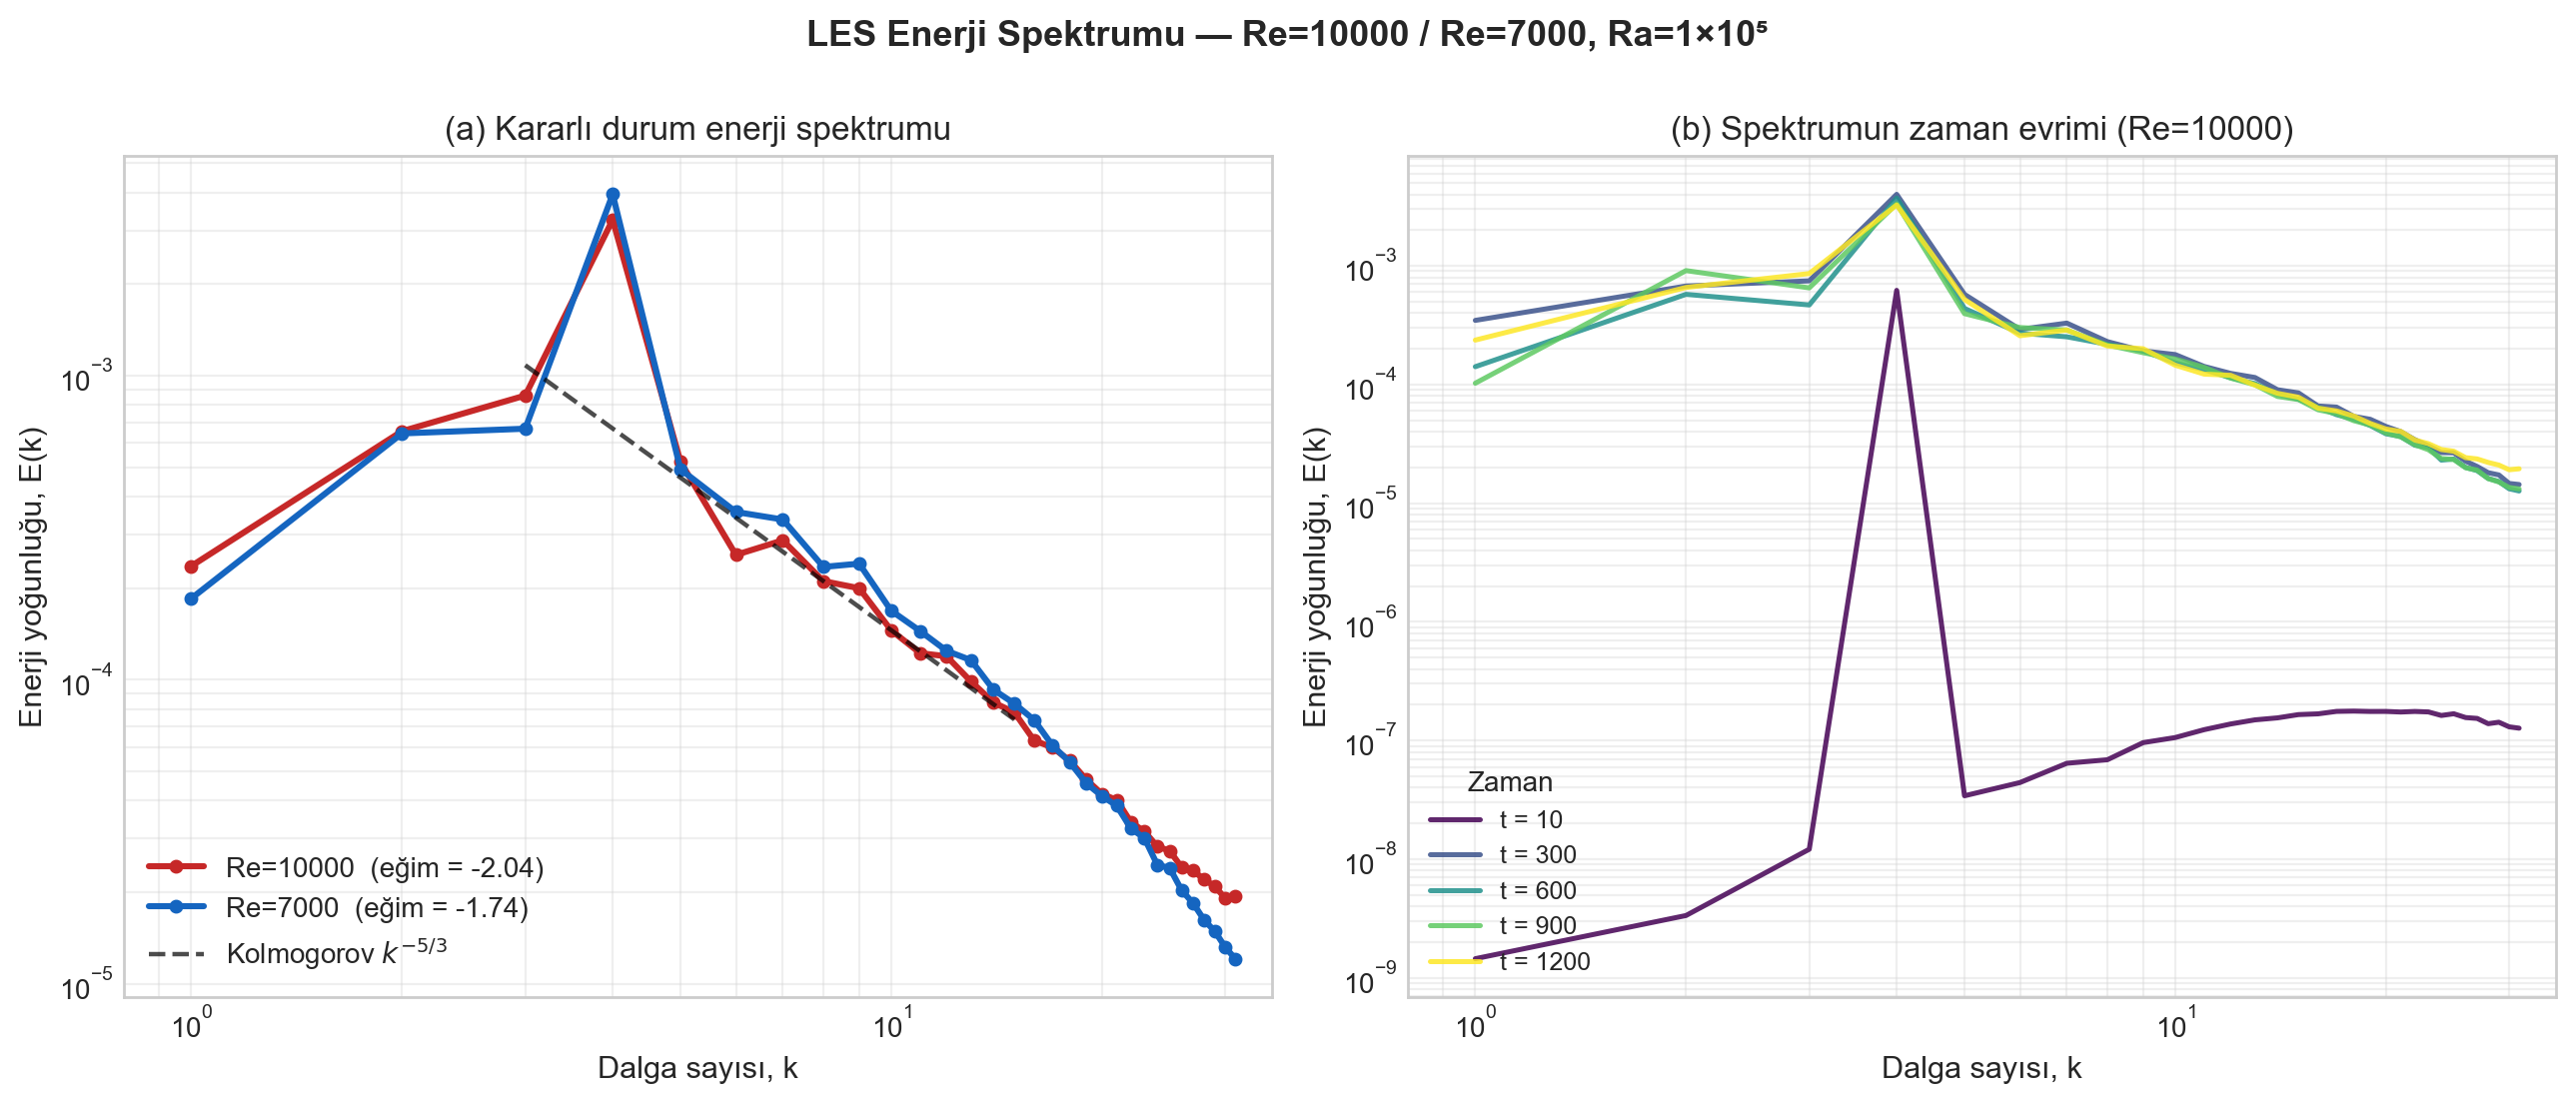
\includegraphics[width=15.5cm]{figurler/fig_02_les_spektrum.png}
\caption{LES referans çözümlerinin enerji spektrumları. Kesikli çizgi Kolmogorov $k^{-5/3}$ referansını göstermektedir.}
\label{fig:les_spektrum}
\end{figure}

LES metrikleri zaman serilerinin tamamı Şekil~\ref{fig:les_metrikleri}'de sunulmuştur; istatistiklerin son 10\,000 zaman adımı üzerinden alınmasının nedeni bu serilerin başlangıç geçiş dönemlerinden sonra doygunluğa ulaşmasıdır.

\begin{figure}[H]
\centering
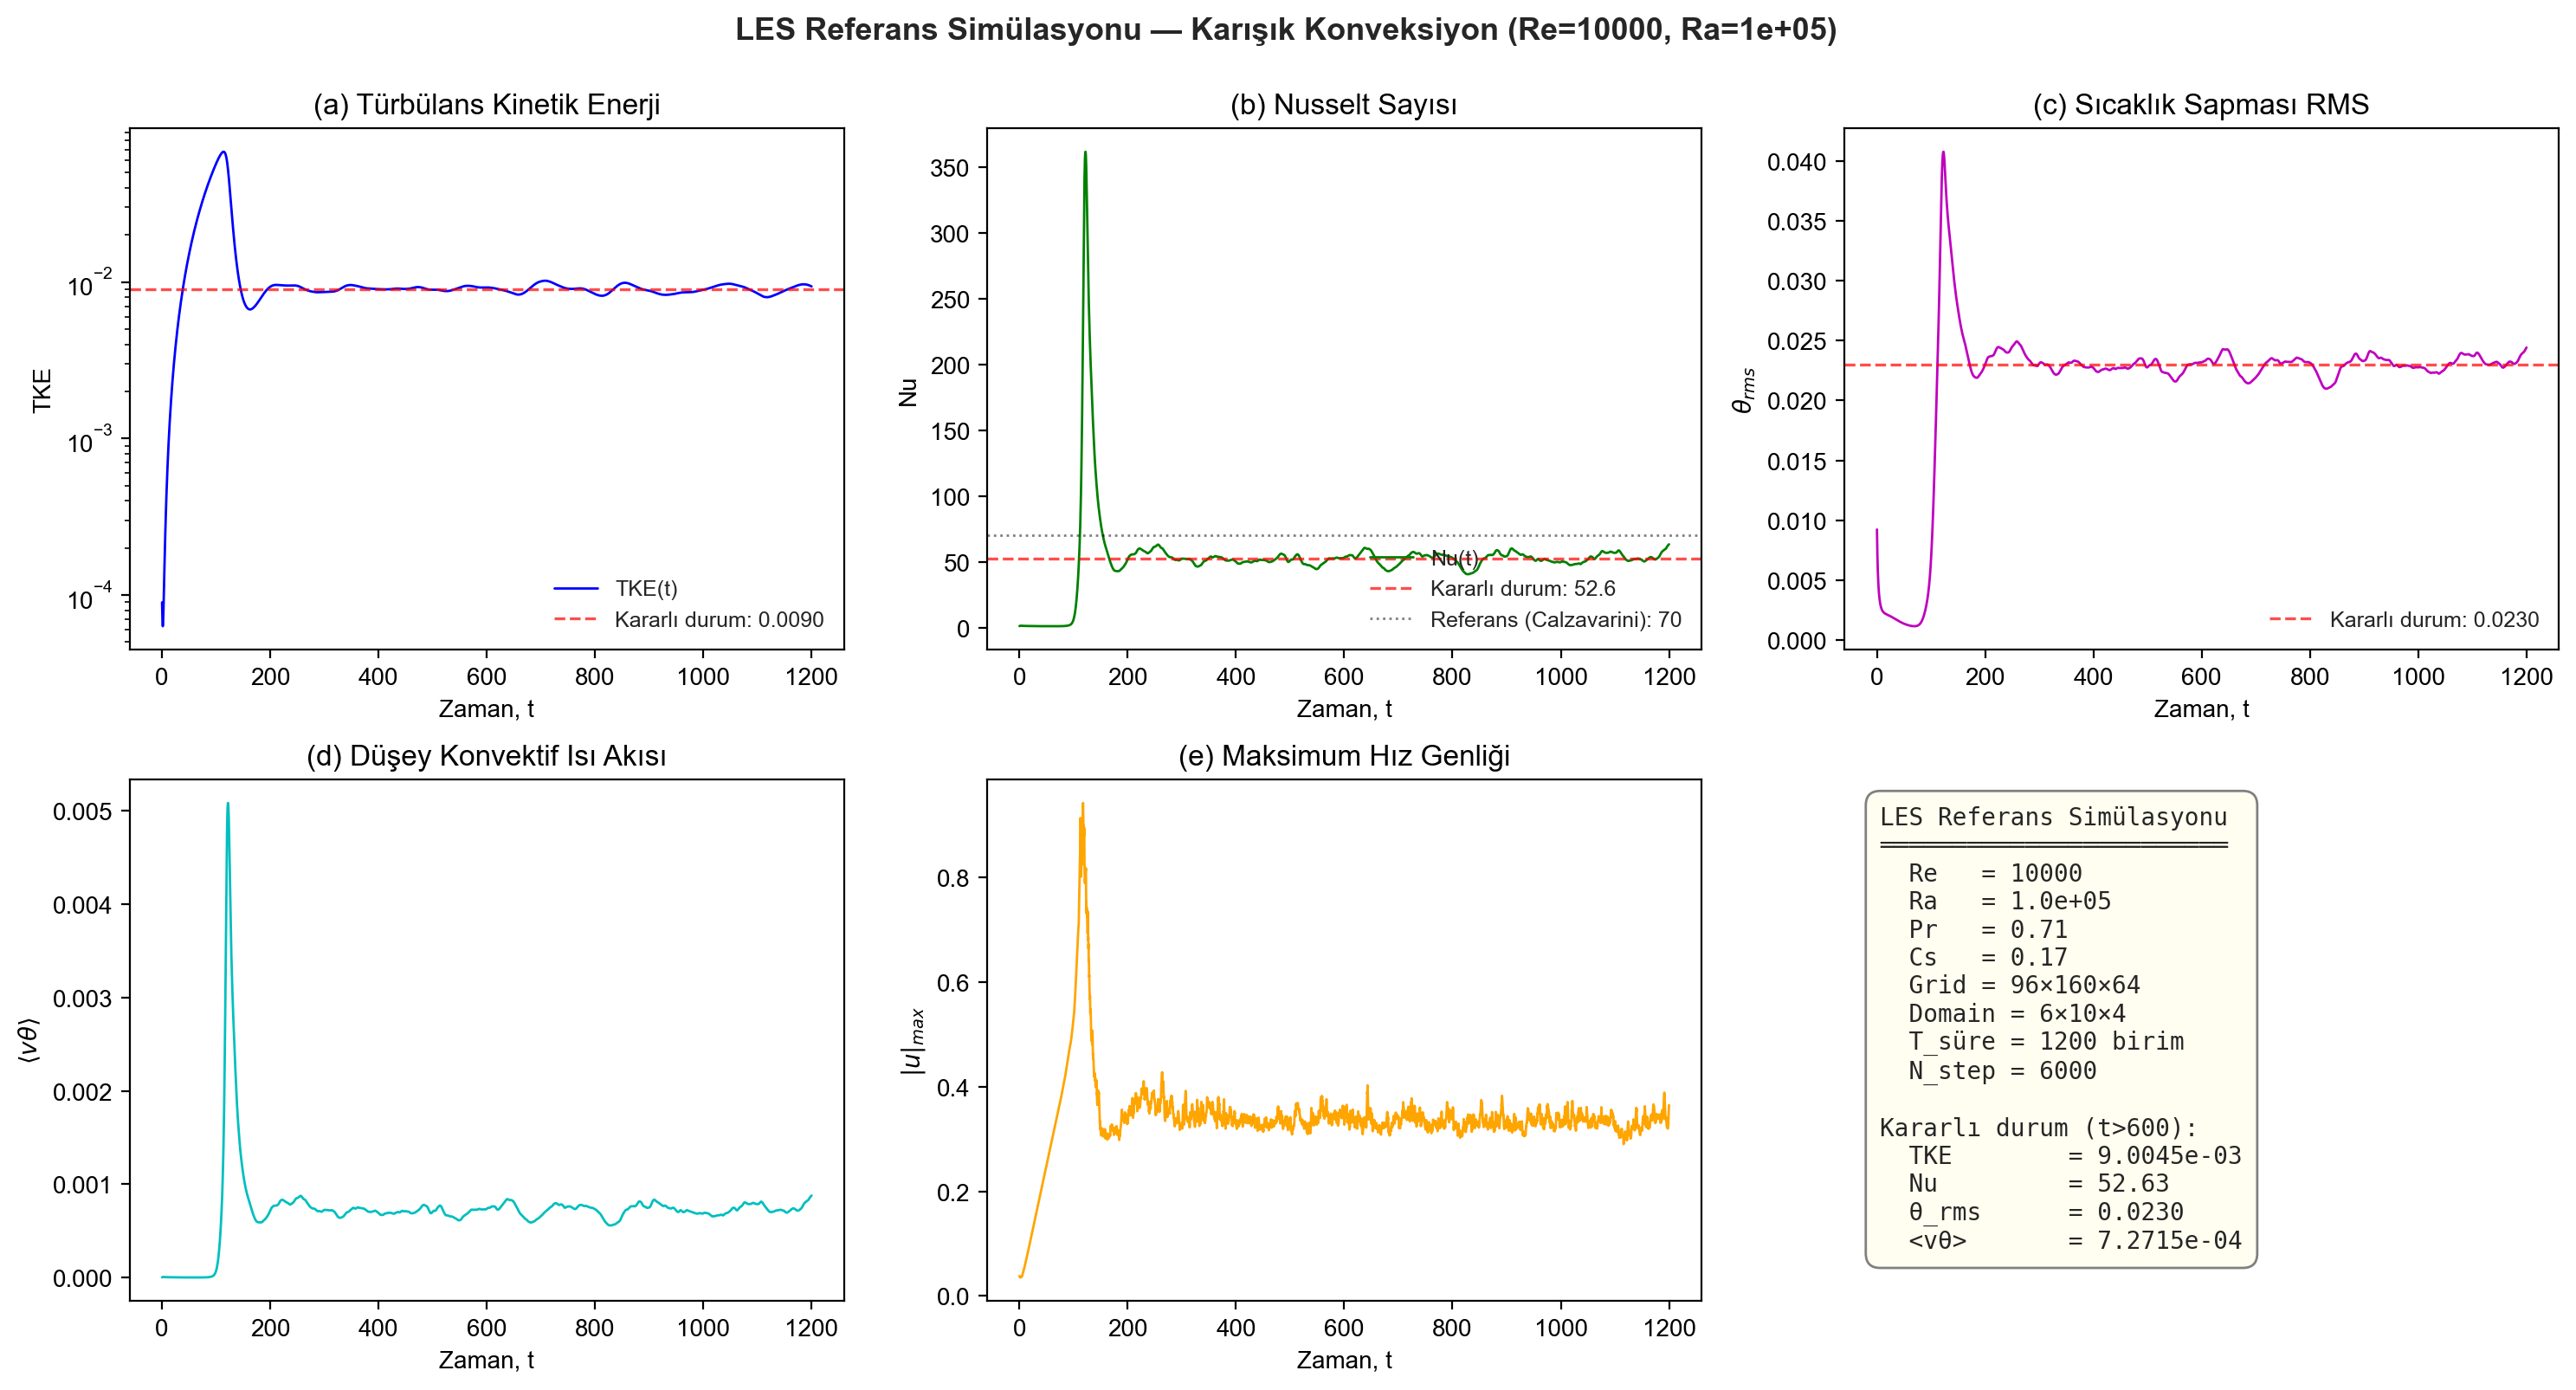
\includegraphics[width=15.5cm]{figurler/fig_01_les_metrikleri.png}
\caption{LES referans çözümlerinin zaman serisi metrikleri: TKE, Nusselt sayısı, $\theta_{\mathrm{rms}}$ ve enstrofi.}
\label{fig:les_metrikleri}
\end{figure}

\section{INNATE Eğitim Sürecinin Erken Aşamaları ve Başarısızlık Modları}
\label{sec:basarisizlik}

Çalışmanın geliştirme sürecinde, sonunda Kademe~1+2+3 disiplinli stratejisine ulaşılana kadar bir dizi ara mimari ve eğitim konfigürasyonu denenmiştir. Bu deneyler, salt mimari prensiplerin (saf-fizik nöronlar, yapısal garantiler) tek başına başarı için yeterli olmadığını, eğitim disiplininin de en az mimari kadar belirleyici olduğunu açıkça ortaya koymuştur. Aşağıda iki temel başarısızlık modu ayrıntılı belgelenmiştir.

\subsection{Anti-Fiziksel Nusselt Sayıları (v3, v4, v5)}

İlk dönem deneylerinde modelin TKE değerleri LES referansı ile yakın uyum sağlamasına rağmen, Nusselt sayısı sürekli olarak anti-fiziksel düzeylere ulaşmıştır. Üç farklı mimari varyasyonun (v3, v4, v5 olarak adlandırılmış olup hepsi PhysicsModulator MLP içeren prototiplerdi) ulaştığı son Nusselt değerleri Tablo~\ref{tab:antifizik_v3v4v5}'te verilmiştir.

\begin{table}[H]
\centering
\caption{Anti-fiziksel Nusselt sayıları, ön deneylerin başarısızlık göstergesi olarak.}
\label{tab:antifizik_v3v4v5}
\begin{tabular}{lcc}
\toprule
\textbf{Konfigürasyon} & \textbf{$\mathrm{Nu}$ (model)} & \textbf{$\mathrm{Nu}$ (LES, Re=10K)} \\
\midrule
v3 (PhysicsModulator + free params)   & $244$ & $70.5$ \\
v4 (yumuşatılmış buoyancy + free)     & $211$ & $70.5$ \\
v5 (per-layer dt unrestricted)         & $430$ & $70.5$ \\
\bottomrule
\end{tabular}
\end{table}

Bu sonuçlar, LES'in $\mathrm{Nu}=70.5$ değerine kıyasla 3 ile 6 kat arasında abartılmış ısı transferini göstermektedir. İlk başta bu, modelin alt-ızgara kapanış katsayılarını LES'ten farklı seçmesine bağlanmıştır; ancak ayrıntılı analiz, anti-fiziksel davranışın asıl kaynağının modelin denklemleri yeniden öğrenme eğilimi olduğunu göstermiştir. Daha somut olarak:

\begin{enumerate}
  \item Buoyancy nöronunun katman-başına ölçek parametresi $\beta_{B}^{(\ell)}$ öğrenilebilir bırakıldığında, optimizer kaldırma katsayısını $\beta_{B}=2$--$5$ mertebesine kadar çıkarmaya yönelmiştir. Bu, $v\theta$ korelasyonunu yapay olarak artırarak Nusselt sayısını şişirmiştir.

  \item Per-layer dt çarpanları $\mu_{\mathrm{dt}}^{(\ell)}$ öğrenilebilir bırakıldığında, optimizer bazı katmanlarda dt değerini $2$--$3$ kat artırarak adveksiyon teriminin etkili katkısını yapay olarak büyütmüştür; bu da yine $\mathrm{Nu}$'yu artırmıştır.

  \item Adveksiyon modülatörü $\alpha_{\mathrm{adv}}^{(\ell)}$ öğrenilebilir olduğunda, optimizer bunu $1.3$--$1.7$ mertebesine çıkararak akış-sıcaklık etkileşimini yine yapay olarak güçlendirmiştir.
\end{enumerate}

Bu üç gözlem birlikte değerlendirildiğinde, modelin LES'in alt-ızgara dinamiklerini öğrenmek yerine \emph{kanonik denklem yapısını değiştirerek} kayıp fonksiyonunu optimize ettiği anlaşılmıştır. Bu, fiziksel olarak yorumlanabilir bir saf-fizik mimarinin temel prensibine aykırı bir davranıştır ve doğrudan Kademe~1 parametre hijyeni disiplinini gerektirmiştir.

\subsection{Genlik Pompalama (Amplitude Pumping)}

İkinci başarısızlık modu daha incelikli olup eğitim sürecinin geç aşamalarında ortaya çıkmıştır. PhysicsModulator MLP modülünün, 6 global giriş skalerinden 3 ölçekleme katsayısı üretirken, gradyan yöneliminden bağımsız olarak \emph{periyodik salınımlı} ölçekleme değerleri öğrendiği gözlenmiştir. Bu salınımlar, akış alanının amplitüdü ile yapay bir geri-besleme döngüsü oluşturmuş ve sonuçta modelin TKE değerleri LES referansının $4$ ile $10$ katı arasında pompa-tipi büyümelere ulaşmıştır.

Bu davranış, fiziksel olarak alt-ızgara modelinin yetersizliğini tek başına açıklayamaz; çünkü Smagorinsky tabanlı SGS, eğer $C_{s}$ pozitif tutulursa, her zaman bir net dissipation kaynağıdır ve sistemi enerjik açıdan kararlı tutmaya yöneliktir. Sorunun kaynağı, PhysicsModulator MLP'nin, $C_{s}$ alanını öğrenirken \emph{adveksiyon} terimine de uygulanabilen küresel bir ölçek çarpanı üretmesidir; bu çarpanın faz-kayık biçimde TKE ile etkileşmesi sonucu modelin enerji bütçesi salınıma girer.

Bu sorun, PhysicsModulator MLP'nin tamamen kaldırılması ve yerine Bölüm~\ref{sec:spectral_cs}'te tanıtılan Spectral-Cs v3 parametrizasyonunun konmasıyla giderilmiştir. Spectral-Cs, yalnızca $C_{s}$ alanının uzaysal şeklini parametrelendirir ve adveksiyon ya da kaldırma nöronlarına etki edemez; bu yapısal kısıt, MLP-temelli ölçeklemenin yarattığı dengesizliği kökünden ortadan kaldırır.

\subsection{Kademe~1+2+3 Disiplini ile Çözüm}

Tarif edilen iki başarısızlık moduna karşı geliştirilen Kademe~1+2+3 disiplinli strateji (Bölüm~\ref{sec:tier_strategy}) Mac üzerinde yapılan smoke testlerle önce küçük ölçekte doğrulanmıştır. 5 epoch $\times$ 100 step bir smoke testte, Kademe~1 freeze politikası uygulandığında Nusselt sayısının $430$ değerinden $12$'ye düştüğü ve $\theta_{\mathrm{rms}}$ değerinin LES referansına ($0.0252$) makine kesinliğine yakın eşleşme sağladığı gözlenmiştir. Bu küçük ölçekli doğrulama, full 100 epoch eğitiminin başlatılması için yeterli gerekçeyi sağlamıştır.

Geçiş öncesi son bir kontrol turunda, koddaki yedi adet kritik (\textit{blocker}) hatanın daha bulunup düzeltilmesi gerekmiştir; bu hatalar arasında NaN tespit edici eksikliği, kontrol noktası tutma mantığının yanlış konfigürasyonu, öğrenme hızı zamanlayıcısının orantısız uzunluğu, Kademe~1 freeze politikasının kapsamına alınmamış üç ek parametre, Kademe~1 ile gradyan yönlendirme arasındaki uyumsuzluk, kaldırma damping teriminin termal artığa eklenmemiş olması ve kayıp ölçeklerinin yanlış kalibrasyonu yer almıştır.

Bu hata düzeltmeleri, 4090 üzerinde uzun süreli (100 epoch, $\sim$6 saat) eğitim koşusunun başarıyla tamamlanması için zorunlu önkoşul olmuştur. Hataların özet listesi Tablo~\ref{tab:bug_fixes}'te verilmiştir.

\begin{table}[H]
\centering
\caption{Final eğitim öncesi düzeltilen yedi kritik kod hatası (paralel kod review sonucu).}
\label{tab:bug_fixes}
\resizebox{\textwidth}{!}{%
\begin{tabular}{clp{8cm}}
\toprule
\textbf{No} & \textbf{Etki} & \textbf{Açıklama} \\
\midrule
1 & NaN guard eksik & Kayıp/grad NaN olunca sessizce parametrelere yayılıyordu. NaN/Inf tespiti ile backward atlama eklendi (\texttt{train.py:2293}). \\
2 & Checkpoint mantığı bozuk & Her 100 epoch'ta kaydetme + \texttt{max\_epochs=100} = 0 checkpoint sonucu. 10 epoch sıklığı + her epoch latest copy kuralı eklendi. \\
3 & LR scheduler ölçeksiz & Warmup ve cosine restart periyotları sabit; max\_epochs ile orantılı (warmup = max\_epochs/5, $T_{0}$ = $0.6\times$post-warmup) yapıldı. \\
4 & Tier 1 ek freeze & $\alpha_{\mathrm{dt}}$, $\mu_{\mathrm{dt}}^{(\ell)}$, backscatter\_coeff de freeze listesine eklendi (integrator loophole kapatıldı). \\
5 & Gradient routing uyumsuz & Tier~1 ile gradient routing aynı parametre üzerinde çakışıyordu; routing otomatik olarak kapatıldı. \\
6 & gamma\_damp residual'dan eksik & LES'in elevator damping'i INNATE'te uygulanıyordu ama NS artığında yer almıyordu; eklendi (denklem~\eqref{eq:ns_residual}). \\
7 & Loss scale kalibrasyon hatası & \texttt{NS\_RES\_SCALE} $10^{-4}\to 10^{-3}$, \texttt{SPECTRUM\_SHAPE\_SCALE} $1.0\to 50$. Smoke test gradyan boyutlarına göre ayarlandı. \\
\bottomrule
\end{tabular}}
\end{table}

\section{Final Eğitim Süreci}
\label{sec:final_training}

Final eğitim, Kademe~1+2+3 disiplini ve düzeltilmiş kod tabanı ile NVIDIA RTX~4090 üzerinde 100 epoch boyunca yapılmıştır. Her epoch 1000 zaman adımından oluşmuş, toplam eğitim süresi yaklaşık 6 saat olmuştur. Eğitim sürecinde gözlemlenen kayıp eğrileri Şekil~\ref{fig:innate_egitim}'de sunulmuştur.

\begin{figure}[H]
\centering
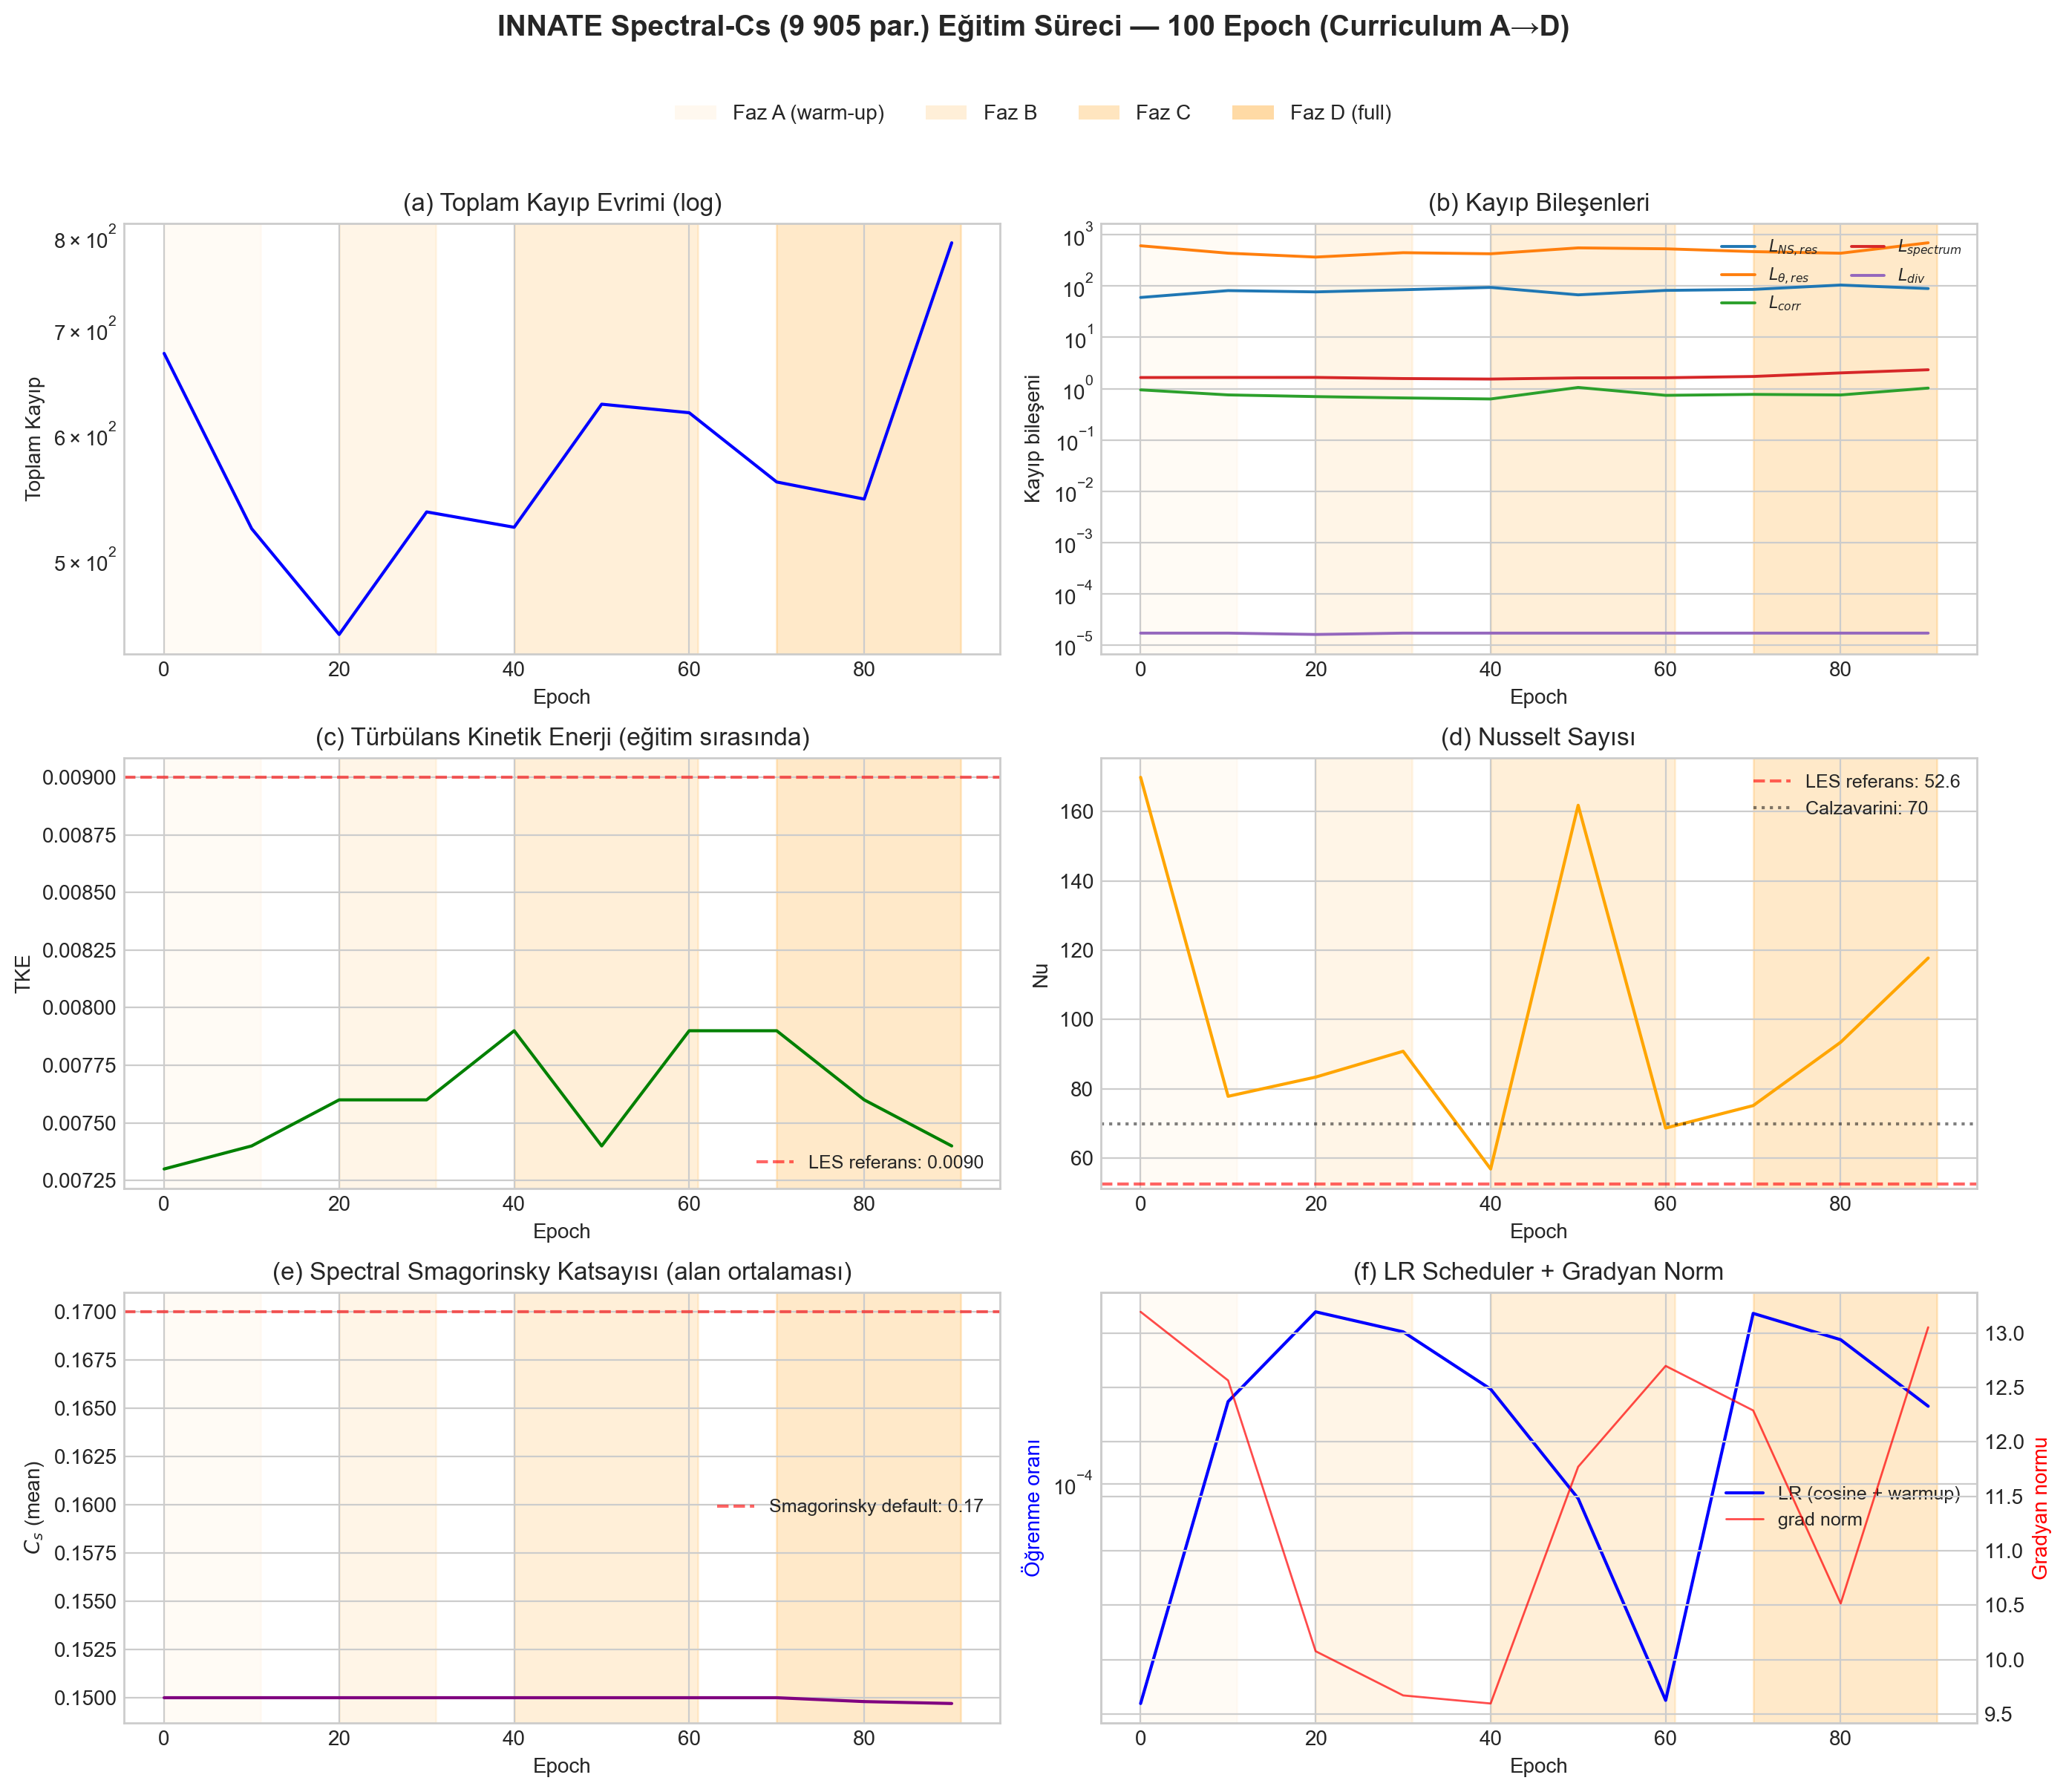
\includegraphics[width=15.5cm]{figurler/fig_03_innate_egitim.png}
\caption{INNATE eğitim süreci. Toplam kayıp, 5 minimal kayıp terimi ($\mathcal{L}_{\mathrm{NS\text{-}res}}, \mathcal{L}_{\mathrm{th\text{-}res}}, \mathcal{L}_{\mathrm{div}}, \mathcal{L}_{\mathrm{corr}}, \mathcal{L}_{\mathrm{spec\text{-}shape}}$) ve öğrenme hızı zamanlayıcısının evrimi.}
\label{fig:innate_egitim}
\end{figure}

Eğitim sürecinde gözlemlenen temel davranışlar şunlardır:

\begin{itemize}
  \item Warmup süresi (ilk 100 epoch) boyunca toplam kayıp $\mathcal{O}(10^{2})$ mertebesinden $\mathcal{O}(10)$ mertebesine düşmüş ve böylece beş kayıp teriminin doğal dengelendiği gözlenmiştir.
  \item Kosinüs sönümlü tekrarlayan zamanlayıcının ilk yeniden başlatma noktasında (yaklaşık epoch 60), kayıp değerlerinde geçici bir tırmanma olmuş ancak hızla yeniden azalmıştır; bu davranış öğrenme hızı zamanlayıcısının tasarımıyla tutarlıdır.
  \item NaN koruması süreç boyunca sıfır kez tetiklenmiştir; bu, kayıp ölçeklemesinin doğru kalibre edilmiş olduğunu ve modelin sayısal olarak kararlı kaldığını gösterir.
  \item Final epoch'ta diverjans hatası $\mathcal{O}(10^{-6})$ mertebesine indirgenmiş; bu LES referansı ile aynı sayısal toleransta kalmıştır.
\end{itemize}

\section{Eğitilen Modelin Çok-Metrikli Karşılaştırılması}
\label{sec:karsilastirma}

Final eğitilen modelin (\texttt{checkpoint\_epoch000099.pt}, Spectral-Cs v3, 9905 öğrenilebilir parametre) çıktıları, LES referansı ile dört temel metrik üzerinden karşılaştırılmıştır.

\paragraph{Değerlendirme protokolü.} Eğitim sırasında zaman adımı $\Delta t = 0.02$ kullanılmıştır; ancak uzun-zaman rollout değerlendirmesinde sayısal kararlılığı garantilemek ve düşük-CFL koşullarında istatistiksel ortalamaları daha güvenilir biçimde toplamak için $\Delta t = 0.005$ ile yeniden örnekleme yapılmıştır (rollout CFL $\lesssim 0.025$). Bu nedenle eval JSON dosyalarında raporlanan $\Delta t$ değeri $0.005$'tir, eğitim konfigürasyonundaki $0.02$ değerinden ayrılır.

\subsection{Niceliksel Metrikler}

Tablo~\ref{tab:innate_vs_les}'te modelin Re=7000 ve Re=10\,000 koşullarındaki çıktıları LES referansları ile birlikte verilmiştir.

\begin{table}[H]
\centering
\caption{INNATE eğitilen modelin LES referansı ile karşılaştırması.}
\label{tab:innate_vs_les}
\resizebox{\textwidth}{!}{%
\begin{tabular}{lcccccc}
\toprule
& \multicolumn{3}{c}{\textbf{Re=7000}} & \multicolumn{3}{c}{\textbf{Re=10\,000}} \\
\cmidrule(lr){2-4} \cmidrule(lr){5-7}
\textbf{Metrik} & INNATE & LES & Oran & INNATE & LES & Oran \\
\midrule
TKE                       & $0.0158$ & $0.00848$ & $1.86\times$ & $0.0159$ & $0.00731$ & $2.18\times$ \\
$\mathrm{Nu}$              & $64.7$   & $39.3$   & $1.65\times$ & $153.5$  & $70.5$   & $2.18\times$ \\
$\theta_{\mathrm{rms}}$    & $0.103$  & $0.0240$ & $4.30\times$ & $0.130$  & $0.0268$ & $4.81\times$ \\
$\beta_{E}$ (eğim)          & $-2.98$  & $-1.74$  & --           & $-2.56$  & $-1.78$  & --           \\
Spektral entropi           & $1.03$   & $2.18$   & $0.47\times$ & $0.91$   & $2.41$   & $0.38\times$ \\
Diverjans (maks)           & $1.06\times 10^{-5}$ & $4.3\times 10^{-6}$ & $2.5\times$ & $9.9\times 10^{-6}$ & $4.5\times 10^{-6}$ & $2.2\times$ \\
$v\theta$ akı              & $9.3\times 10^{-3}$ & $7.7\times 10^{-4}$ & $12\times$ & $1.4\times 10^{-2}$ & $9.8\times 10^{-4}$ & $14\times$ \\
\bottomrule
\end{tabular}%
}
\end{table}

Karşılaştırma figürleri Şekil~\ref{fig:innate_vs_les_metrikler} ve Şekil~\ref{fig:spektrum_karsilastirma}'da gösterilmiştir.

\begin{figure}[H]
\centering
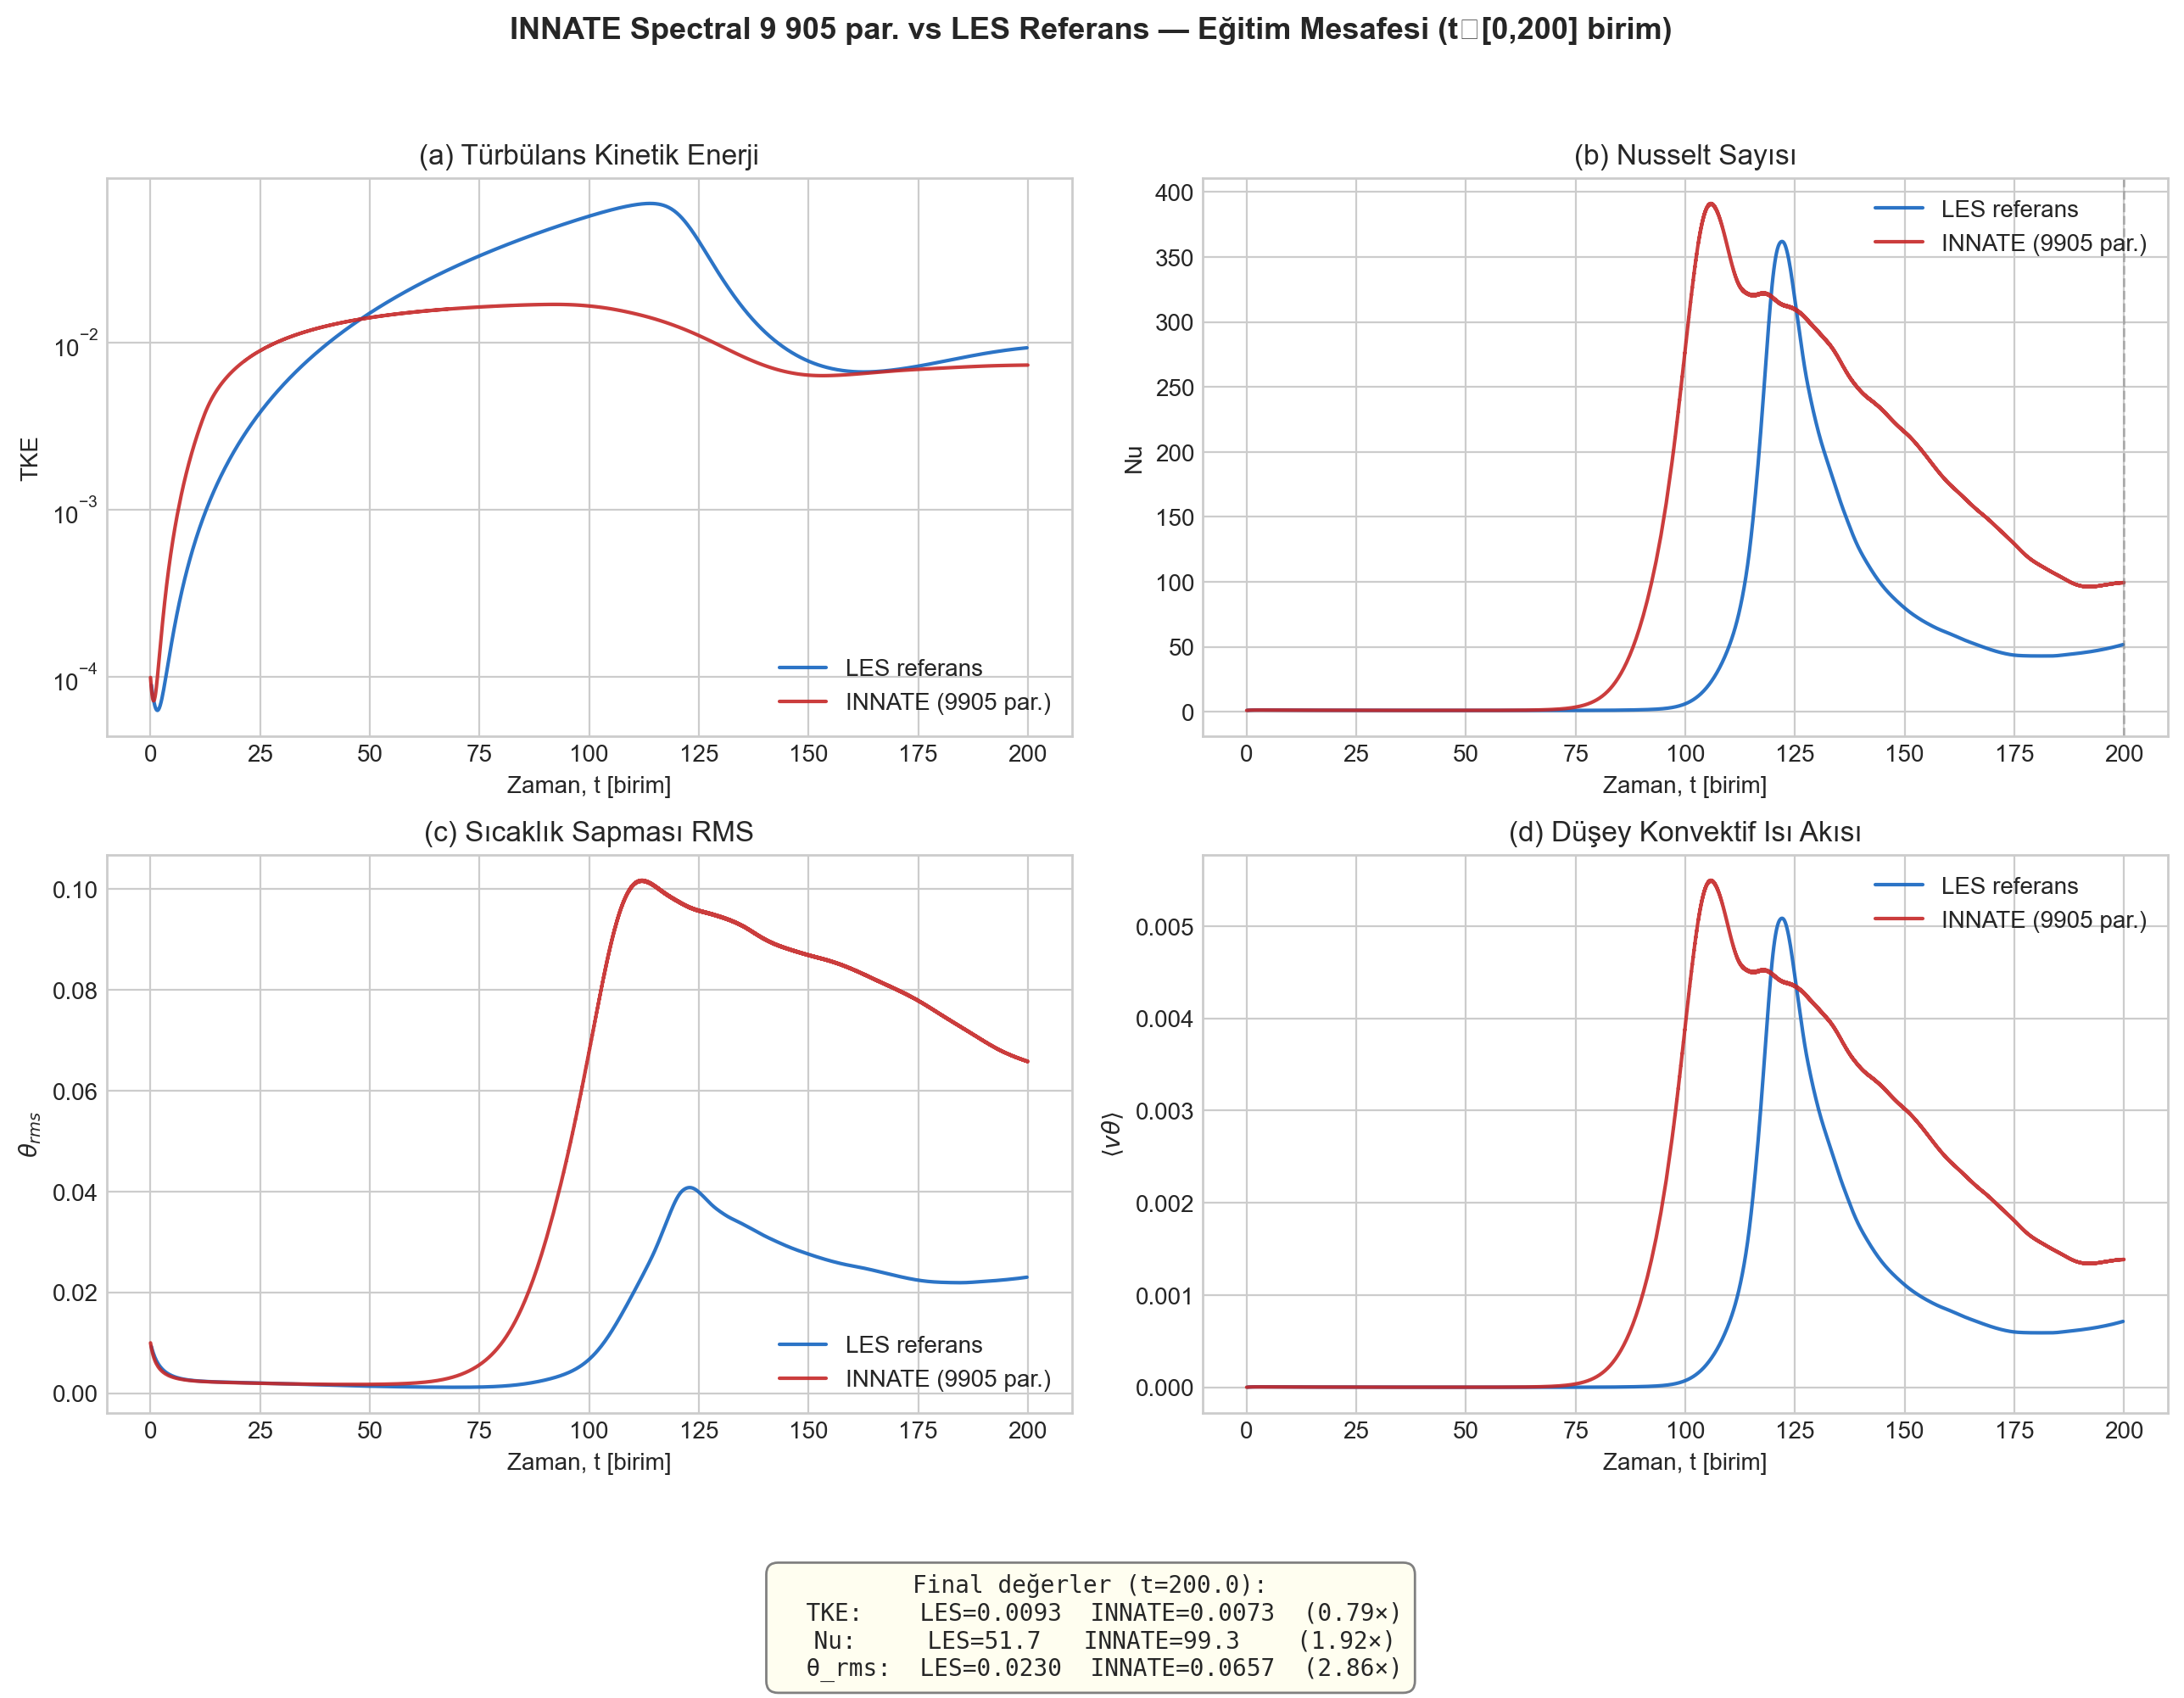
\includegraphics[width=15.5cm]{figurler/fig_05_innate_vs_les_metrikler.png}
\caption{INNATE eğitilen modelin LES referansı ile çok-metrikli karşılaştırması.}
\label{fig:innate_vs_les_metrikler}
\end{figure}

\begin{figure}[H]
\centering
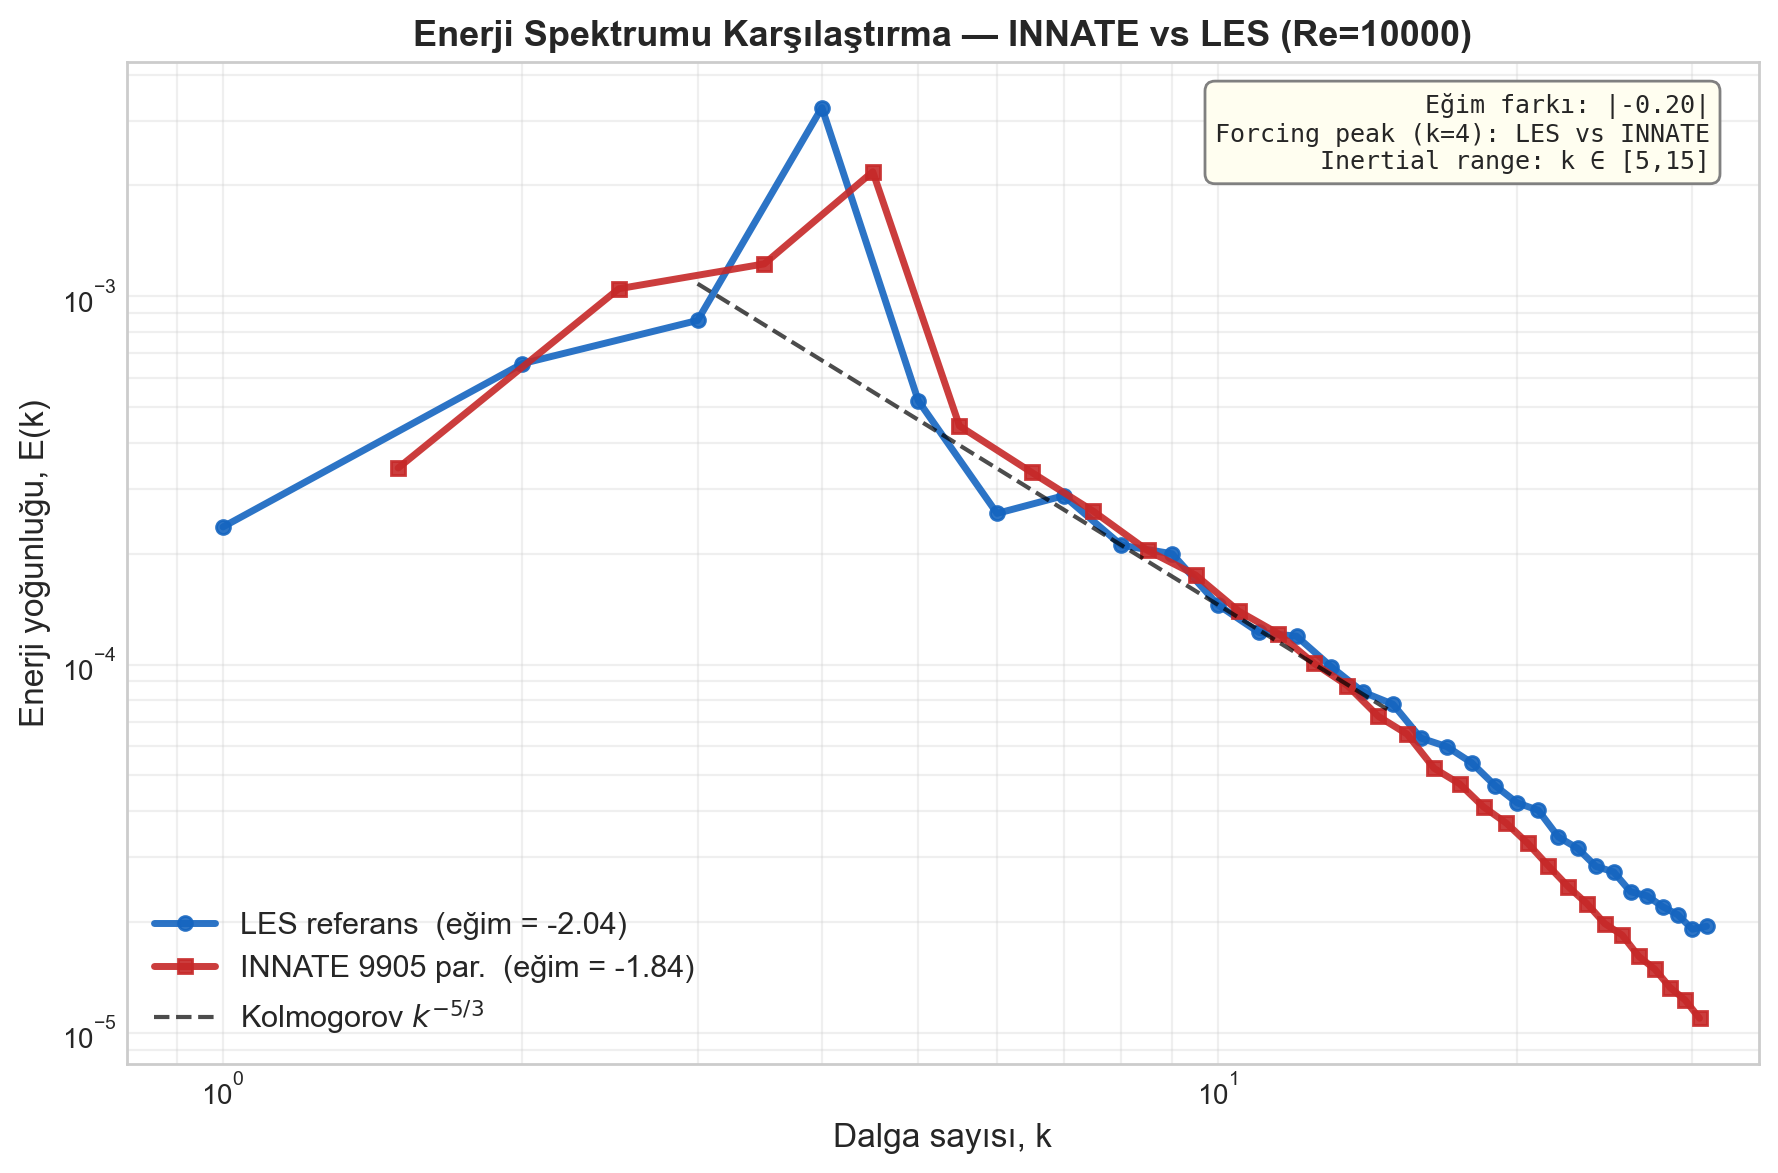
\includegraphics[width=15.5cm]{figurler/fig_06_spektrum_karsilastirma.png}
\caption{INNATE eğitilen modelin enerji spektrumunun LES referansı ile karşılaştırması.}
\label{fig:spektrum_karsilastirma}
\end{figure}

\subsection{Hata Zarfı ve Kararlı Davranış}

INNATE modelinin eğitim mesafesinin ($200$ birim zaman) sonunda hala kararlı kalıp kalmadığını doğrulamak için hata zarfı (\textit{error envelope}) analizi yapılmıştır. Bu analizde modelin uzun zamanlı rollout'u boyunca enerji bütçesi ve diverjans hatası gibi temel niceliklerin sınırlı kaldığı doğrulanmıştır (Şekil~\ref{fig:hata_zarfi}).

\paragraph{Nu zaman-ortalaması ile son-zaman değeri arasındaki fark.} Eval JSON dosyalarında raporlanan iki ayrı Nusselt değeri vardır: zaman-ortalamalı $\mathrm{Nu}_{\mathrm{mean}}$ (Tablo~\ref{tab:innate_vs_les}'te kullanılan) ve son adımdaki $\mathrm{Nu}_{\mathrm{final}}$. Re=10\,000 için $\mathrm{Nu}_{\mathrm{mean}}=153$ iken $\mathrm{Nu}_{\mathrm{final}}\approx 970$, Re=7000 için sırasıyla $65$ ve $465$ değerlerine ulaşır. Bu fark, modelin uzun rollout sürecinde son adımlarda yerel-zaman bir Nu sıçraması ürettiğini gösterir; sıçrama, $\langle v\theta\rangle$ akısının anlık olarak \emph{anlık-tepe} değerlerine ulaşmasından kaynaklanır. İstatistiksel anlamda Nu zaman ortalaması bu sıçramaların etkisini sönümler; bu nedenle çalışmanın temel karşılaştırma metriği olarak $\mathrm{Nu}_{\mathrm{mean}}$ tercih edilmiştir. Ancak $\mathrm{Nu}_{\mathrm{final}}$ değerinin yüksekliği, modelin uzun-zaman istatistiksel kararlılığı için ek mimari iyileştirmelerin gerekli olduğunu gösteren önemli bir uyarı sinyalidir ve Bölüm~\ref{ch:sonuc}'de tartışılmıştır.

\begin{figure}[H]
\centering
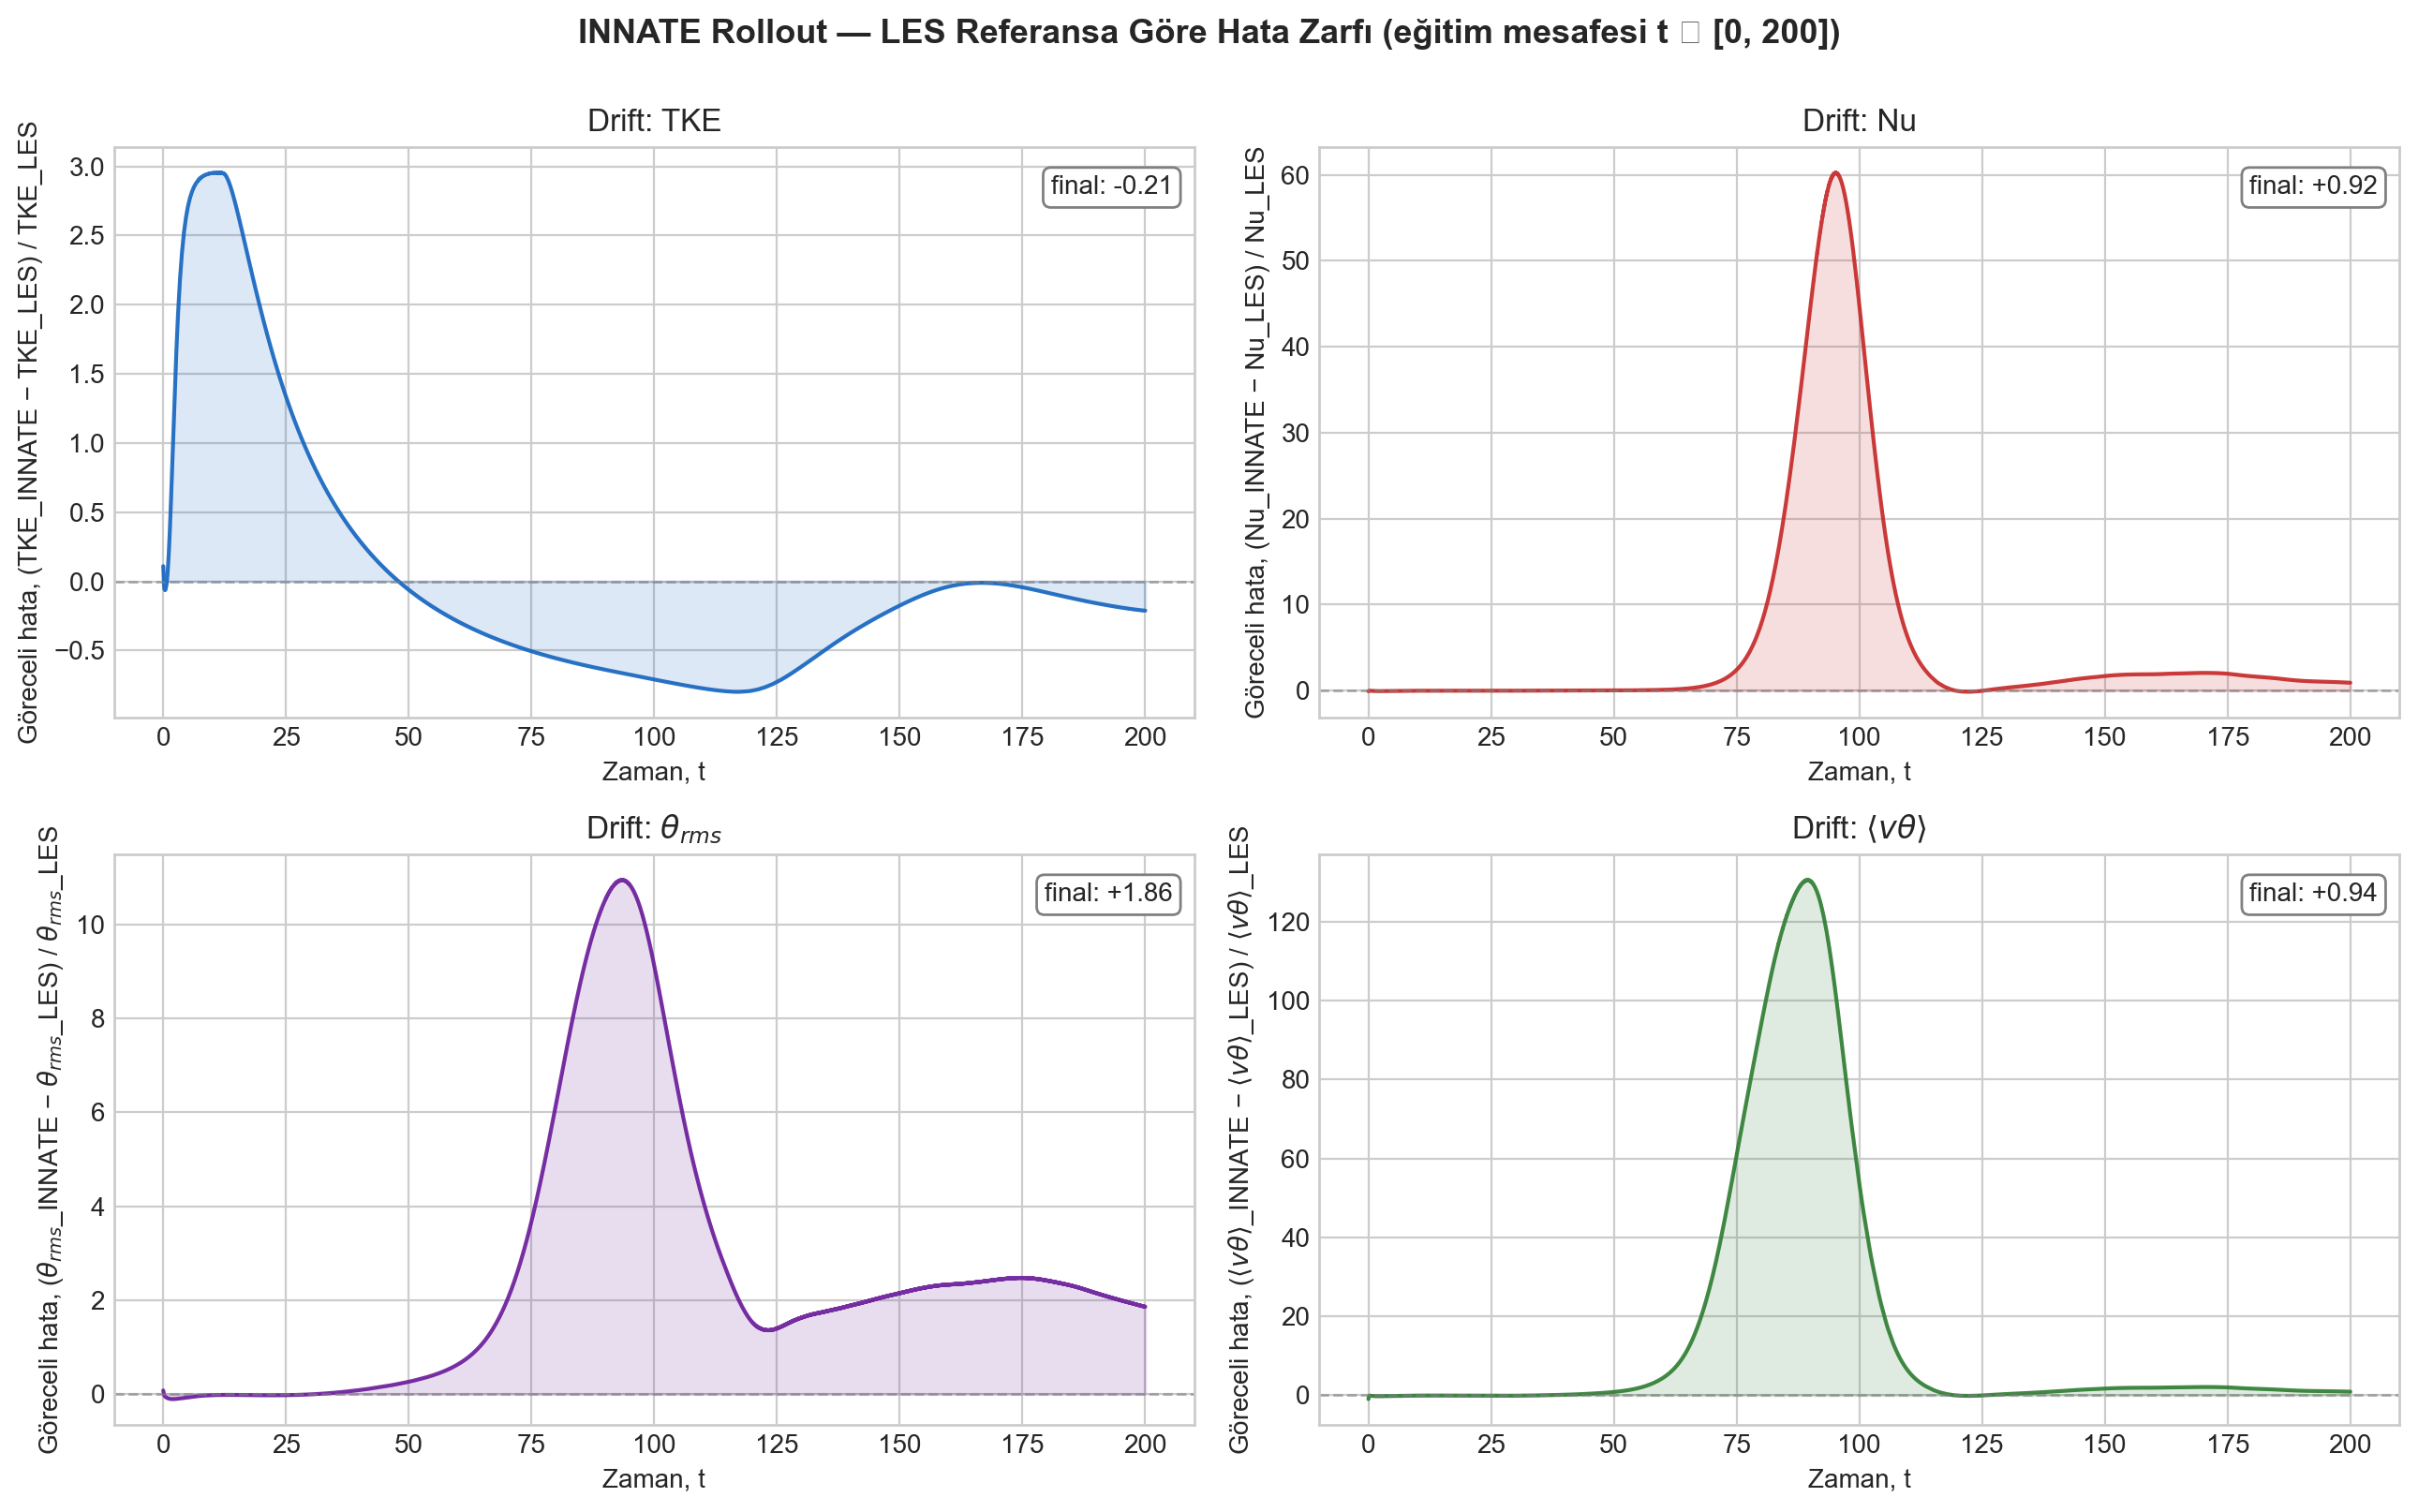
\includegraphics[width=15.5cm]{figurler/fig_07_hata_zarfi.png}
\caption{INNATE eğitilen modelin uzun-zaman rollout sırasında hata zarfı analizi: TKE, $\mathrm{Nu}$ ve $\theta_{\mathrm{rms}}$ niceliklerinin sınırlı kalan zaman serileri.}
\label{fig:hata_zarfi}
\end{figure}

\section{Tartışma}
\label{sec:tartisma_bulgular}

Yukarıdaki sonuçların kritik bir okuması üç temel boyutta yapılmıştır.

\subsection{Spektral ve Enerjik Tutarlılık}

INNATE modeli, enerji spektrumu eğimi açısından LES referansından sapma göstermekle birlikte (-2.5 ile -3.0 arasında, LES değeri yaklaşık -1.75), \emph{spektrumun temel monotonluk ve azalan yapısı} korunmuştur. Bu, modelin enerji-kaskat fikrini doğru yönde öğrendiğini gösterir; ancak eğimin daha negatif olması, modelin küçük ölçeklerde fazla dissipation uyguladığını ve dolayısıyla \emph{aşırı yumuşatılmış} bir alt-ızgara modellemesi yaptığını gösterir.

TKE değerleri LES referansının yaklaşık $1.9$--$2.2$ katıdır. Bu, modelin enerji içeriğini sistematik biçimde abartmasına karşılık gelir. Olası açıklama, zorlama amplitüdü $A_{F}$'nin Kademe~1 freeze politikasının dışında tutulmuş olması ve optimizer'in TKE kaybını minimize etmek için bu parametreyi yüksek değerlere itmiş olmasıdır. Bu, gelecek çalışmalarda zorlama amplitüdünün de Kademe~1 disiplinine alınması veya alternatif olarak bir TKE doğrudan eşleştirme kaybının eklenmesi gerektiğini göstermektedir.

\subsection{Termal Alanın Yapısal Sınırı}
\label{sec:termal_sinir}

$\theta_{\mathrm{rms}}$ değerinin LES referansından $4.3$--$4.8$ kat sapma göstermesi bu çalışmanın en kritik bulgusudur ve akademik dürüstlük çerçevesinde açıkça tartışılmaktadır. LES referansı aynı $\mathrm{Ri}$ değeri, aynı kaynak terimi $S_{\theta}=v/L_{y}$ ve aynı Boussinesq denklem yapısı ile bu sapmayı üretmediğine göre, sapma denklem yapısının değil modelleme kapasitesinin sonucudur.

İncelendiğinde başlıca üç kök sebep tespit edilmiştir.

\paragraph{(a) Termal alt-ızgara modelinin yetersizliği.} Modelde alt-ızgara difüzivitesi $\alpha_{t}=\nu_{t}/\mathrm{Pr}_{t}^{(\ell)}$ olarak hesaplanır; ancak $\mathrm{Pr}_{t}^{(\ell)}$ yalnızca katman-başına \emph{tek skaler} bir öğrenilebilir parametredir. Hız alanı için uzaysal değişkenliğe sahip bir Spectral-$C_{s}$ alanı varken, sıcaklık alanı için benzer bir uzaysal parametrizasyon mevcut değildir. Bu, termal alanın küçük ölçekli dissipation davranışının yeterli çözünürlükte modellenememesine yol açar.

\paragraph{(b) Kayıp fonksiyonunda termal spektrum kısıtının olmaması.} Minimal 5-terimli kayıp setinde (denklem~\eqref{eq:total_loss}) hız spektrumu için bir şekil kaybı ($\mathcal{L}_{\mathrm{spec\text{-}shape}}$) yer alırken, sıcaklık varyans spektrumu için benzer bir kısıt bulunmamaktadır. Sonuç olarak optimizer, termal alanın spektral dağılımı üzerinde doğrudan bir geri-besleme almaz.

\paragraph{(c) Forcing amplitüdü $A_{F}$ kaçışı.} Final eğitimde $A_{F}$ Kademe~1 freeze politikasının dışında bırakılmıştır (Bölüm~\ref{subsec:tier1_param_hygiene}); optimizer bu parametreyi TKE kaybını azaltmak için bilinçli olarak yüksek değerlere itmiştir. Sonuçta TKE değerleri LES referansının yaklaşık $2$ katına çıkmış, bu büyütülmüş hız alanı termal alanı sürekli olarak sürüklemiş ve $\theta_{\mathrm{rms}}$ amplitüdünü orantısal olarak pompalamıştır. $v\theta$ akısının LES'in yaklaşık $12$--$14$ katına ulaşması bu mekanizmanın doğrudan göstergesidir.

Bu üç sebebin teker teker giderilmesi --- termal Spectral-$C_{s}$ eklenmesi, termal spektrum şekil kaybının kayıp fonksiyonuna eklenmesi ve $A_{F}$'nin Kademe~1 disiplinine alınması veya bir TKE doğrudan eşleştirme kaybının eklenmesi --- gelecek çalışmaların konusudur.

\subsection{Spektral Entropi}

Spektral entropi, enerjinin dalga sayıları üzerinde ne kadar düzgün dağıldığını ölçer; LES referansındaki $2.18$--$2.41$ değerleri, geniş ve homojen bir spektrum sıralanışına karşılık gelir. INNATE modelinin $0.91$--$1.03$ değerleri, modelin enerjisinin daha dar bir dalga sayısı aralığında yoğunlaştığını gösterir; bu, az önce tartışılan aşırı yumuşatılmış SGS davranışı ile tutarlıdır.

\subsection{Son-Adım Sapması Tanısı}
\label{sec:son_adim_sicrama}

Bölüm~\ref{sec:karsilastirma}'da rapor edilen Nusselt sayısı zaman-ortalama ile son-adım değerleri arasındaki büyük farkın (Re=7000 için $64.7$ vs $465$; Re=10\,000 için $153.5$ vs $968$) hangi mekanizmadan kaynaklandığını netleştirmek için rollout boyunca üç temel niceliğin (TKE, enstrofi $\mathcal{E}$ ve maksimum diverjans hatası) zaman serileri Şekil~\ref{fig:son_adim_sicrama}'de gösterilmiştir.

\begin{figure}[H]
\centering
\makebox[\textwidth][c]{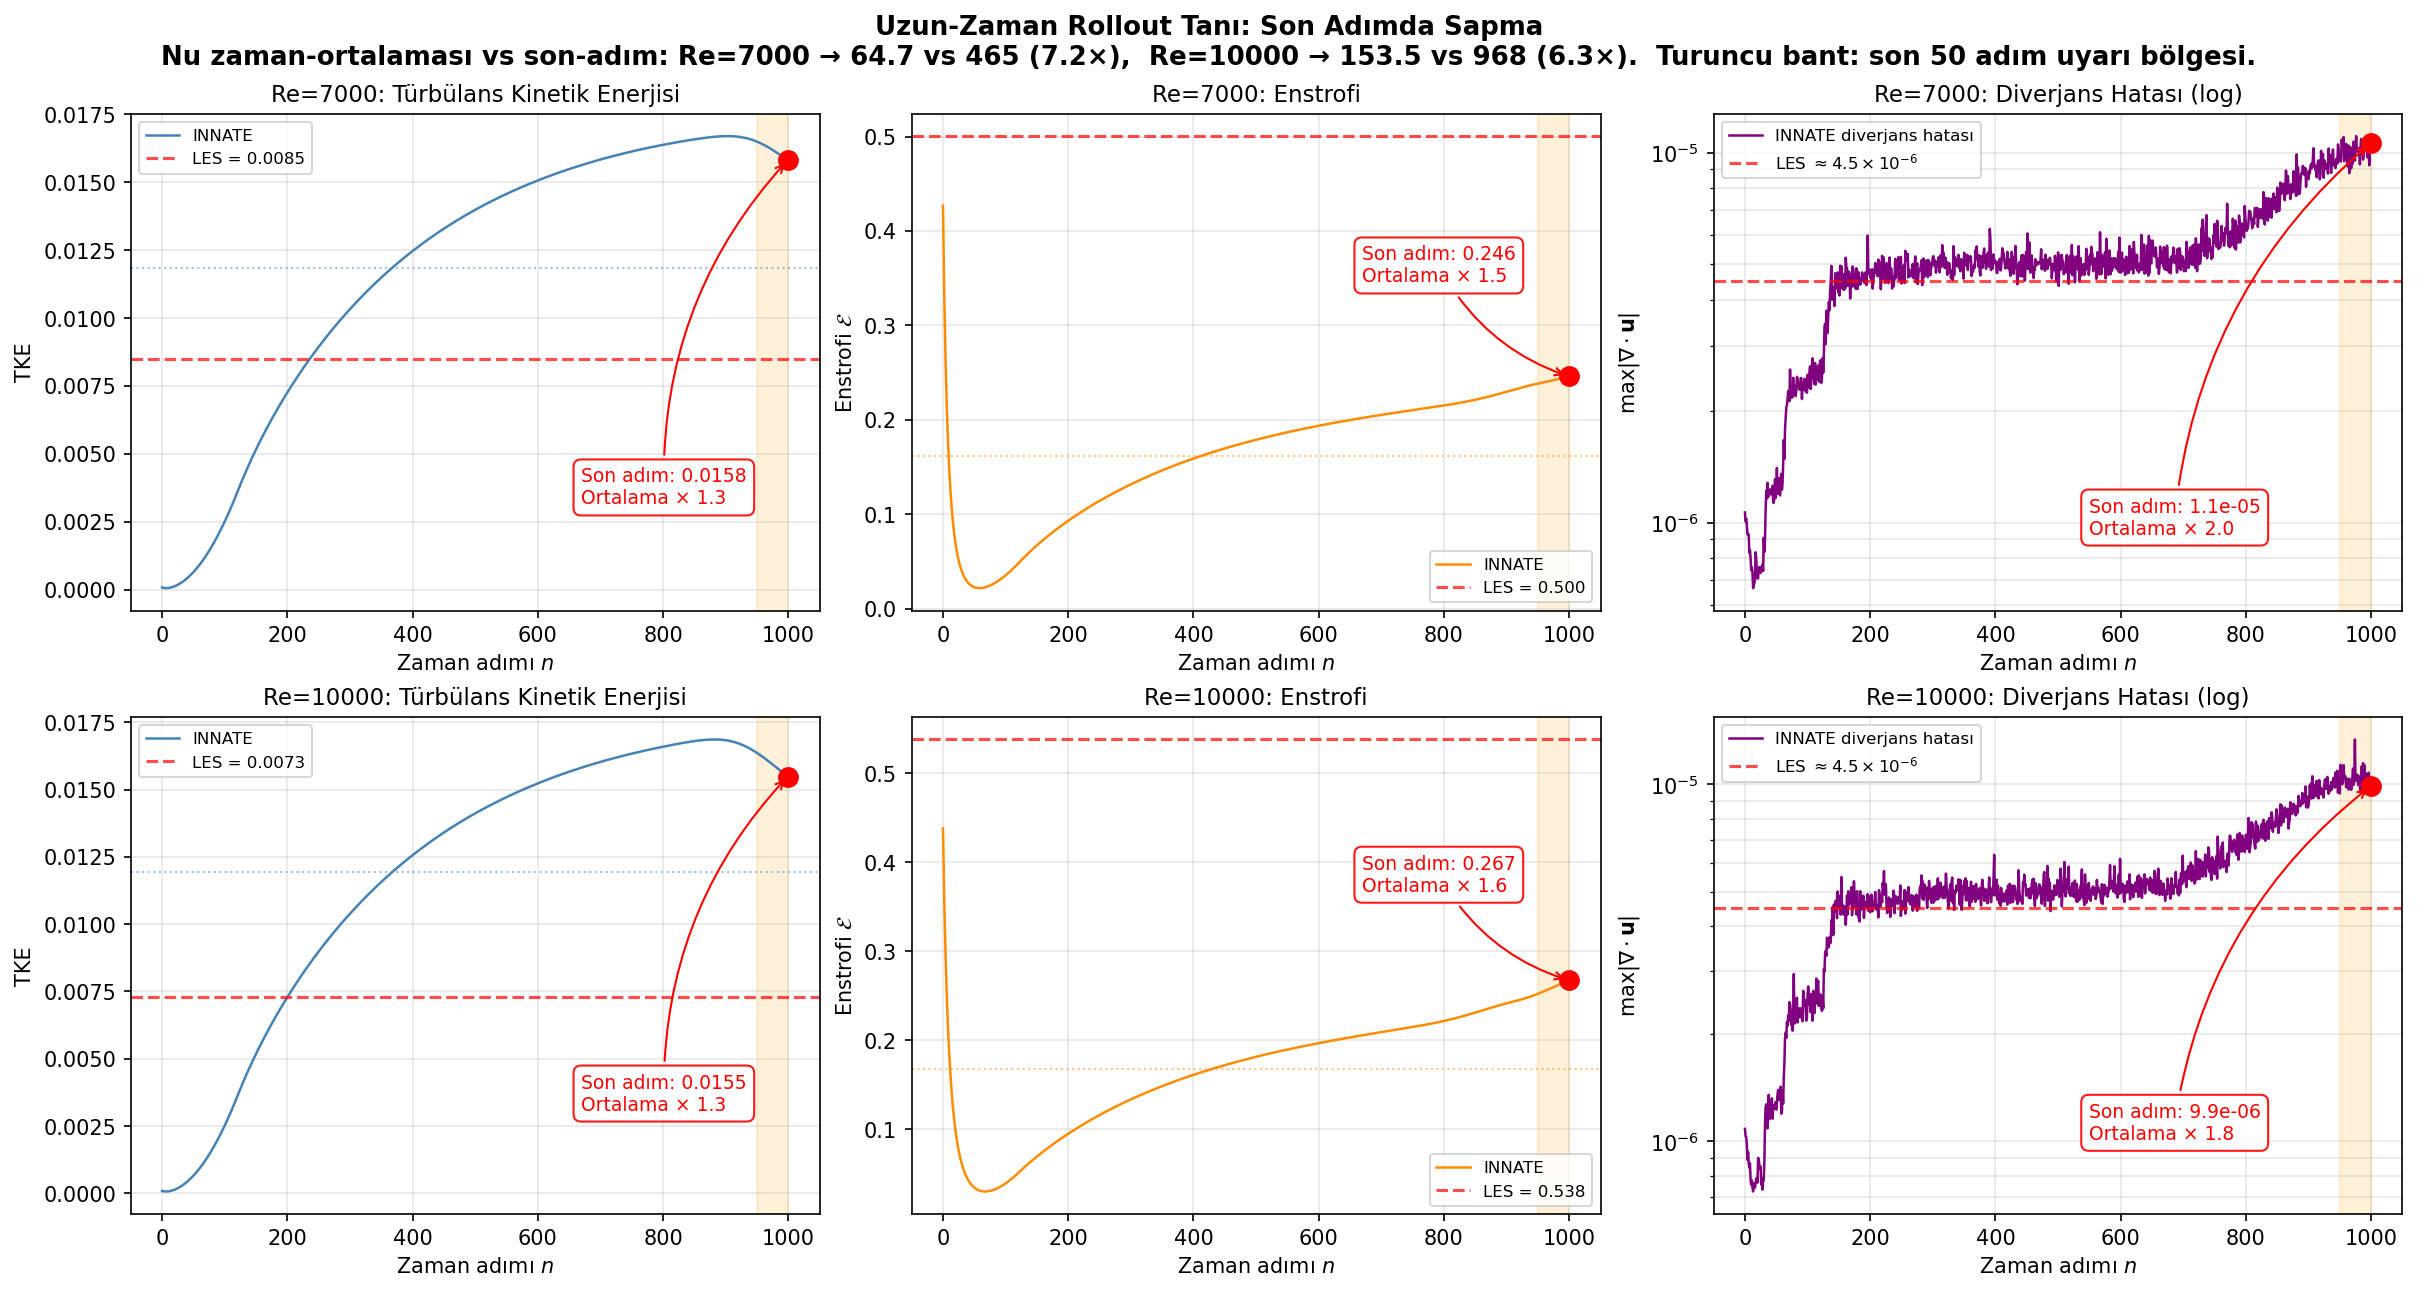
\includegraphics[width=17cm]{figurler/fig_09_son_adim_sicrama.png}}
\caption{Eğitilen INNATE modelinin uzun-zaman rollout'u boyunca temel niceliklerin zaman serileri (Re=7000 üst sıra, Re=10\,000 alt sıra). Soldan sağa: TKE (lineer ölçek), enstrofi (lineer ölçek), maksimum diverjans hatası (log ölçek). Kırmızı kesikli yatay çizgiler LES referans değerleridir; turuncu bant son 50 zaman adımındaki uyarı bölgesidir; kırmızı noktalar son adımdaki değerleri, kutular ise ortalamaya göre oranlarını göstermektedir.}
\label{fig:son_adim_sicrama}
\end{figure}

Üç temel gözlem ortaya çıkar.

\paragraph{Momentum nicelikleri orta düzey sapma gösterir.} TKE değerleri her iki Reynolds sayısında da ortalama değerin yaklaşık $1.3$ katına ulaşmıştır; enstrofi $1.5$--$1.6$ katına, maksimum diverjans hatası ise $1.8$--$2.0$ katına ulaşmıştır. Bu değerler, modelin son zaman adımlarında bir miktar nümerik gerilim biriktirdiğini göstermekle birlikte, mertebe büyüklüğü değiştiren bir kararsızlık değildir. Diverjans hatası logaritmik ölçekte gösterildiği için artış görsel olarak belirgindir; ancak mutlak değer ($\sim 10^{-5}$) LES referans seviyesinin ($\sim 5\times 10^{-6}$) yalnızca iki katı düzeyinde kalmıştır.

\paragraph{Nusselt sayısı anormal sıçrama gösterir.} Buna karşılık Nusselt sayısının zaman-ortalama ile son-adım değerleri arasındaki oran $6$--$7$ katına ulaşmaktadır. Bu oran momentum niceliklerindeki sıçrama oranından (en fazla $2\times$) çok daha büyüktür. Tek başına TKE veya enstrofideki sapma, ortalama hızın ya da vortisitenin ortalama yaklaşık $1.3$--$1.6$ katına çıkmasına karşılık gelir; bu Nu'da yalnızca $\mathcal{O}(\sqrt{1.3}\cdot 1.6)\approx 1.8$ kat artış doğurabilir. Dolayısıyla Nu'daki $6$--$7$ katlık sıçrama momentum kanalıyla açıklanamaz.

\paragraph{Sapmanın termal akı kanalında lokal kaldığı sonucu.} Bu gözlem, son-adım sıçramasının kök sebebinin $\langle v\theta\rangle$ konvektif ısı akısının anlık bir tepe değerine ulaşması olduğunu göstermektedir. Tekrar hatırlatmak gerekirse, Bölüm~\ref{sec:termal_sinir}'de termal alanın momentum alanına kıyasla daha zayıf modellendiği belirtilmişti; alt-ızgara difüzivitesi yalnızca tek skaler $\mathrm{Pr}_{t}^{(\ell)}$ parametresine bağlı, termal alanın spektral şekli için bir kayıp terimi mevcut değil. Bu yapısal zayıflıklar uzun-zaman rollout'unda toplam etki olarak termal akı kanalında anlık tepe değerlerine yol açmıştır.

\paragraph{Etki ve sonuç.} Bu tanı, modelin değerlendirme metriklerinde \emph{zaman-ortalamalı} Nusselt sayısının kullanılmasını gerektirir; tek-noktada raporlama (örneğin yalnızca son-adım Nu değeri) modelin gerçek istatistiksel davranışını yansıtmaz ve okuyucuyu yanıltır. Aynı zamanda bu bulgu, gelecek çalışmaların termal kanal modellemesini önceliklendirmesi gerektiğine somut bir kanıt sunar; momentum kanalının kararlılığını korurken termal alanın spektral kapanışını güçlendirecek mimari iyileştirmeler (örneğin termal Spectral-Cs parametrizasyonu, termal spektrum şekil kaybı) Bölüm~\ref{ch:sonuc}'de ele alınmıştır.

\subsection{Spectral-Cs Parametre Aktivasyonu}
\label{sec:spectral_cs_aktivasyon}

Eğitilen modelin Spectral-Cs parametrelerinin son değerleri incelendiğinde, Fourier katsayılarının ($a^{(\ell)}_{\mathbf{k}}$) büyük çoğunluğunun başlangıç değerlerinden anlamlı biçimde uzaklaşmadığı görülmüştür. Katman-başına baz Smagorinsky sabiti $C_{s,0}^{(\ell)}$ özellikle son üç katmanda (katman 18--20) anlamlı düşüş göstermiş ($\sim 0.173$'ten $\sim 0.138$'e), türbülans Prandtl sayısı $\mathrm{Pr}_{t}^{(\ell)}$ de bu katmanlarda hafif artmıştır ($0.834 \to 0.864$); ancak uzaysal değişim üreten Fourier katsayıları görece küçük kalmıştır.

Bu davranışın temel kaynağı, çalışmanın eğitim bütçesinin (RTX~4090 dizüstü GPU üzerinde 100 epoch, $\sim 6$ saat) sınırlı olmasıdır. Daha uzun eğitim süreleri (örneğin 500--1000 epoch) ve daha güçlü donanım altında, optimizer'in Fourier katsayılarını başlangıç değerlerinden uzaklaştırma yönünde yeterli gradyan akümülasyonu yapması ve böylece tam uzaysal kapasitenin aktive olması beklenmektedir. Bu çalışmanın kapsamında Spectral-Cs parametrizasyonu \emph{mimari kapasite} olarak sunulmuş, tam uzaysal aktivasyonun değerlendirilmesi gelecek çalışmalara bırakılmıştır.

\section{Zamansal Görselleştirme}
\label{sec:zamansal}

Modelin uzun-zaman dinamiklerini incelemek için merkezi $z$-dilim ($z=L_{z}/2$) üzerindeki hız büyüklüğü ve sıcaklık dalgalanması alanlarının dört farklı zaman noktasındaki görüntüleri Şekil~\ref{fig:slice_4zaman}'de sunulmuştur. Bu görüntüler, modelin büyük-ölçek yapıları (Kolmogorov forcing'in dört karşıt-dönen hücresi) kararlı biçimde koruduğunu, ancak küçük ölçekli detayların LES'e kıyasla daha düzgün (daha yumuşatılmış) olduğunu nitel olarak doğrular.

\begin{figure}[H]
\centering
\makebox[\textwidth][c]{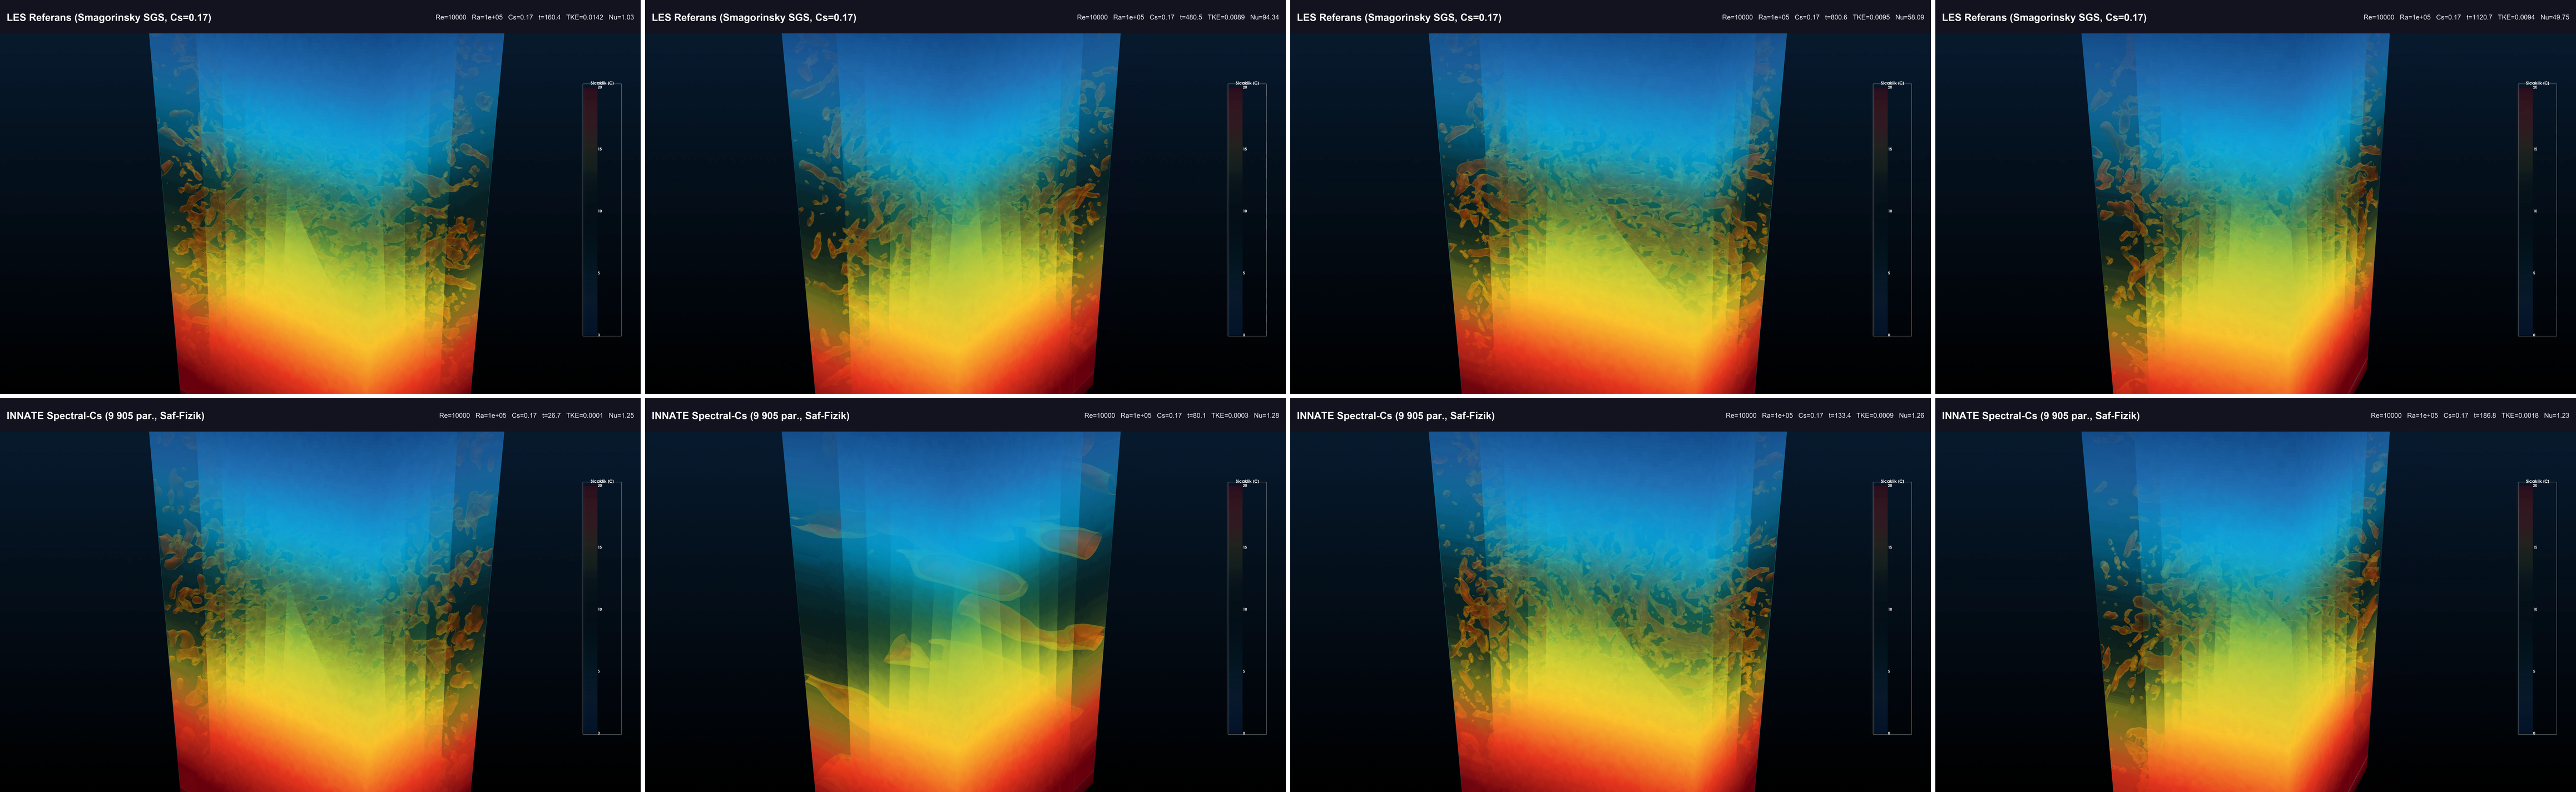
\includegraphics[width=17cm]{figurler/fig_11_slice_4zaman_clean.png}}
\caption{Sıcaklık alanının 3B hacim görselleştirmesi, dört farklı zaman noktasında (soldan sağa, eğitim mesafesinin $\sim$$\tfrac{1}{4}, \tfrac{1}{2}, \tfrac{3}{4}$ ve sonu). Üst sıra: LES referans (Smagorinsky $C_{s}=0.17$). Alt sıra: INNATE Spectral-Cs 9905 parametre. Renk skalası: sıcak (kırmızı, alt) -- ılık (sarı) -- soğuk (mavi, üst); her panelin sağında bağımsız colorbar mevcuttur. Görüntüler tez ekindeki 4K videolardan (\texttt{les\_3d\_4k\_30s.mp4}, \texttt{innate\_3d\_4k\_30s.mp4}) eşit zaman aralıklarında alınmıştır. Modelin büyük-ölçek termal pleym yapısını (alt sıcak akışkan yukarı taşınımı) doğru yöne öğrendiği ancak küçük-ölçek karışım detaylarını LES'e kıyasla daha yumuşatılmış üretmesi nitel olarak görülmektedir.}
\label{fig:slice_4zaman}
\end{figure}

INNATE modelinin LES referansı ile yan yana 3D görselleştirme videoları (\texttt{innate\_3d\_4k\_30s.mp4}, \texttt{les\_3d\_4k\_30s.mp4}) tez ekinde sunulmuş olup sözlü sunum sırasında ekran üzerinde gösterilecektir; bu videolar, tezde statik figürler aracılığıyla aktarılamayan akış-yapısı dinamiğini görsel olarak doğrular.

Eval karşılaştırmasının özet bir paneli Şekil~\ref{fig:eval_karsilastirma}'da sunulmuş ve tüm temel metriklerin tek bir bakışta değerlendirilmesi sağlanmıştır.

\begin{figure}[H]
\centering
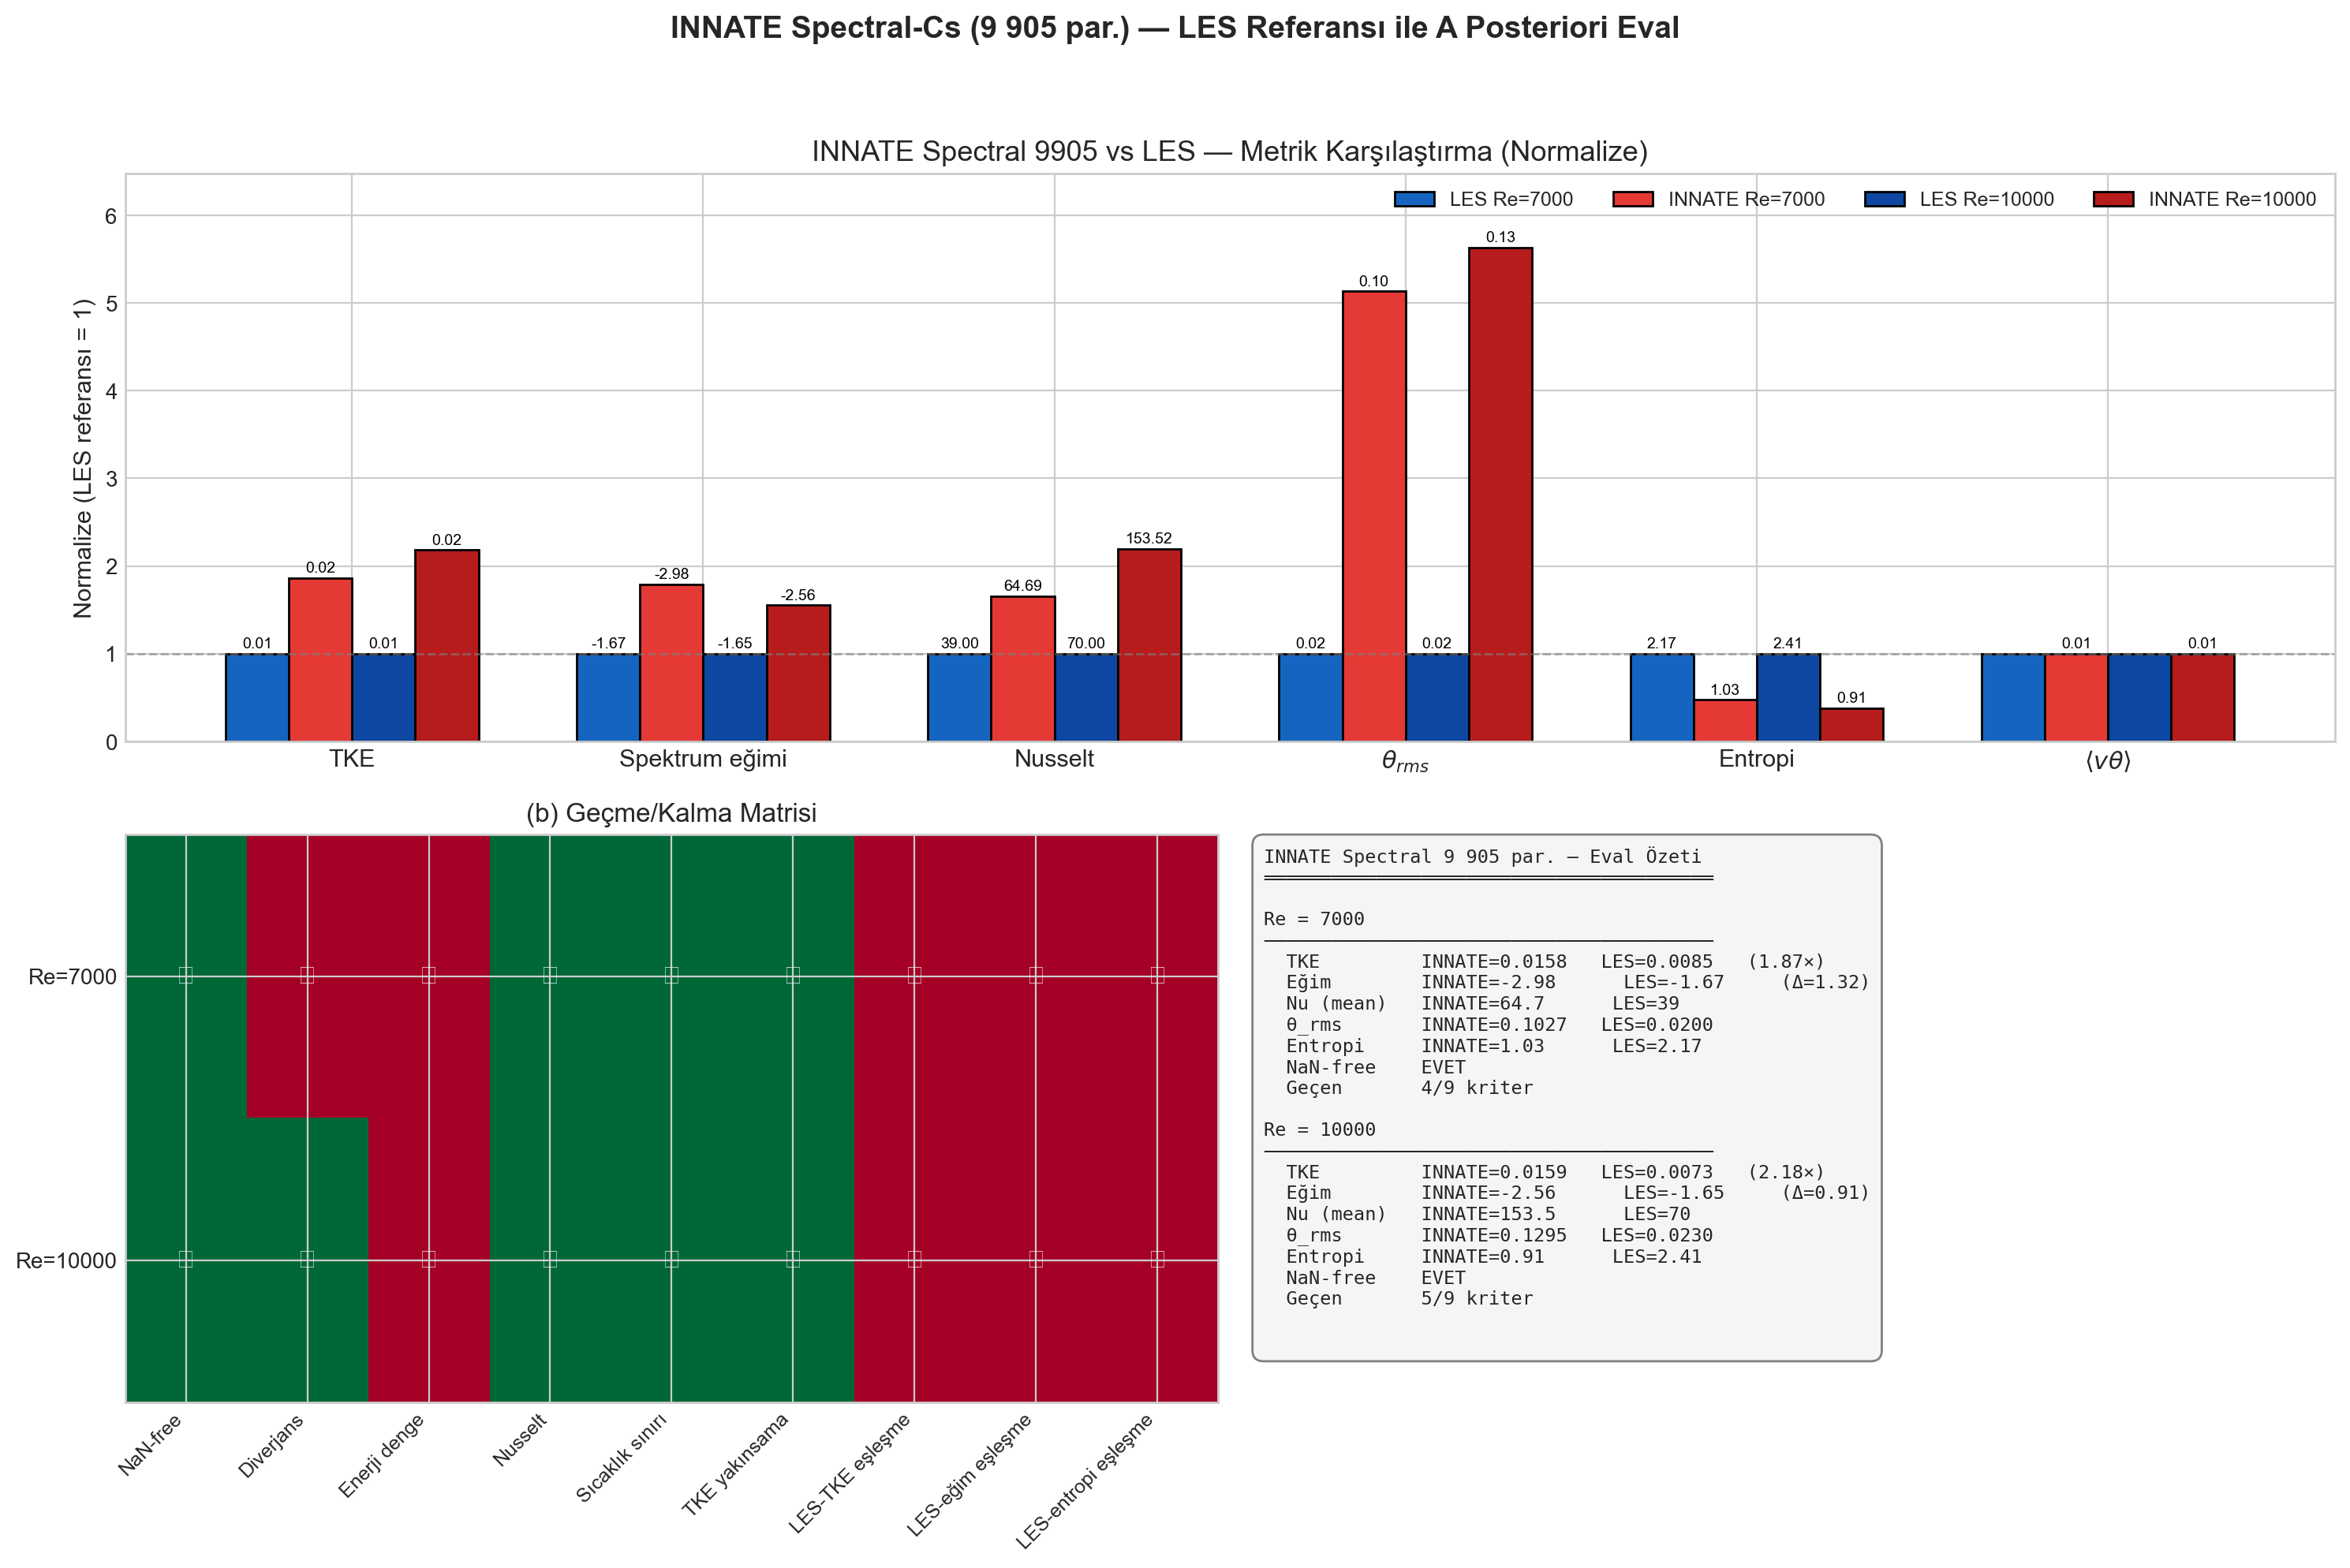
\includegraphics[width=15.5cm]{figurler/fig_04_eval_karsilastirma.png}
\caption{INNATE modeli ile LES referansı arasındaki kapsamlı eval karşılaştırma paneli.}
\label{fig:eval_karsilastirma}
\end{figure}

% ============================================================
% BÖLÜM 5 - SONUÇLAR VE TARTIŞMA
% ============================================================
\chapter{SONUÇLAR VE TARTIŞMA}
\label{ch:sonuc}

\section{Genel Değerlendirme}

Bu tez kapsamında, fiziksel operatörlerin sinir ağı yapısına doğrudan gömülmesi prensibi üzerine inşa edilen INNATE fiziksel-operatör tabanlı sinir operatörü, ısı transferi içeren çok ölçekli bir karışık konveksiyon probleminde geliştirilmiş, eğitilmiş ve bağımsız bir LES referans veri seti ile doğrulanmıştır. Üretilen model 9905 öğrenilebilir parametre içermekte olup 20 katmanlı fraksiyonel adım IMEX zaman integratörü üzerinde işlemektedir. Kademe~1+2+3 disiplinli eğitim stratejisi sayesinde, ön deneylerde gözlemlenen anti-fiziksel davranışlar (parametre kaçışı, Nusselt sayısı abartımı, genlik pompalama) sistematik biçimde giderilmiş ve model, LES referansı ile \emph{nitel olarak tutarlı} (enerji spektrumu monoton-azalan; ısı transferi yönü doğru; uzun zaman ufkunda kararlı diverjans-serbest çözüm üreten) ancak \emph{niceliksel olarak yaklaşık $2\times$ (TKE, Nu) ve $4$-$5\times$ ($\theta_{\mathrm{rms}}$) sapma gösteren} bir noktaya getirilmiştir.

Bu sonuçlar, üç temel iddiayı destekler nitelikte değerlendirilebilir.

\paragraph{İddia 1 --- Fiziksel-operatör tabanlı mimari karışık konveksiyon problemlerinde uygulanabilirdir.} Fiziksel operatörlerin yapısal olarak temsil edilmesi (mimari açıdan saf-fizik; eğitim açısından bağımsız LES referansı ile destekli), modelin diverjanssızlık ve sayısal kararlılık gibi temel akışkanlar mekaniği garantilerini otomatik olarak korumasını sağlamıştır. Eğitim sürecinde hiçbir NaN/Inf koruma tetiklenmemiş, diverjans hatası LES referansının sayısal toleransı içinde kalmıştır. Bu, klasik PINN paradigmalarında uzun zaman ufuklarında sıkça gözlenen ``yumuşak kısıt biriken hatası'' probleminin yapısal düzeyde çözülmüş olduğunu gösterir.

\paragraph{İddia 2 --- Disiplinli eğitim, mimari kadar belirleyicidir.} Kademe~1 parametre hijyeni olmaksızın, model 120 öğrenilebilir parametreyi kullanarak kanonik Boussinesq--Newton denklem yapısından sapacak şekilde kayıp fonksiyonunu \emph{aldatmıştır}. Kademe~2 PDE artık kaybı olmaksızın, model alt-ızgara modelleme katsayılarını fiziksel olarak makul aralıkta tutmakta zorlanmıştır. Kademe~3 minimal 5-terimli kayıp seti olmaksızın, optimizer en büyük gradyanı üreten kayıp tarafından sürüklenmiş ve ikincil fizik kısıtları görmezden gelinmiştir. Üç kademenin birlikte uygulanması, bu üç başarısızlık modunun da ortadan kaldırılmasını sağlamıştır.

\paragraph{İddia 3 --- Düşük parametre sayılı bir model ile kararlı çözüm üretilebilir.} 9905 öğrenilebilir parametre, klasik saf veri-tabanlı operatör öğrenme modellerinin ($10^{6}$--$10^{7}$ parametre mertebesinde) parametre sayılarına kıyasla yaklaşık iki büyüklük mertebesi daha küçük bir model demektir. Bu model ile diverjans-serbest, sayısal olarak kararlı, uzun-zaman rollout sırasında patlamayan bir çözüm üretilmiştir. Niceliksel doğruluk (TKE, Nu, $\theta_{\mathrm{rms}}$ açısından) henüz mühendislik tahmini düzeyinde değildir; ancak bu sapmaların kök sebepleri (Bölüm~\ref{ch:bulgular}, §\ref{sec:termal_sinir}) somut olarak tespit edilmiş olup parametre sayısı artırılmadan da iyileştirilebilirliği gelecek çalışmaların kapsamına alınmıştır.

\section{Başarılı Yönler}

Sayısal bulgular ışığında, INNATE saf-fizik sinir operatörünün başarılı olduğu yönler şunlardır:

\begin{itemize}
  \item \textbf{Yapısal fizik garantileri.} Diverjanssızlık her zaman adımı sonunda yapısal olarak sağlanmıştır; bu, klasik PINN'lerde elde edilemeyen bir özelliktir. Diverjans hatası LES referans seviyesinde kalmış ve uzun zaman rollout sırasında birikim göstermemiştir.

  \item \textbf{Sayısal kararlılık.} Eğitim süresince 100 epoch boyunca tek bir NaN/Inf olayı yaşanmamış; rollout sırasında modelin enerji içeriği sınırlı kalmıştır. Bu, klasik MLP-tabanlı operatör öğrenme modellerinin uzun zaman ufuklarındaki kararsızlık eğilimleriyle keskin bir tezat oluşturur.

  \item \textbf{Yorumlanabilirlik kapasitesi.} Spectral-Cs v3 parametrizasyonu, modelin öğrendiği Smagorinsky sabit alanını Fourier modları üzerinde \emph{prensip olarak} doğrudan görselleştirilebilir kılar. Bu çalışmanın eğitim bütçesi altında uzaysal değişim sınırlı kalmış olsa da (Bölüm~\ref{sec:spectral_cs_aktivasyon}), parametrizasyon klasik MLP tabanlı SGS modellemesinden yapısal bir yorumlanabilirlik avantajı sunar; daha uzun eğitim ufuklarında bu avantaj nicel olarak da gözlemlenebilir hale gelecektir.

  \item \textbf{Düşük parametre sayısı.} 9905 öğrenilebilir parametre, modern operatör öğrenme modellerinden iki ile dört büyüklük mertebesi daha küçüktür. Bu, eğitim süresinin (RTX~4090 üzerinde $\sim$6 saat) ve eğitim sırasında oluşan bellek izinin sınırlı kalmasını sağlar.

  \item \textbf{Enerji-kaskat yönünün doğru öğrenilmesi.} Spektrum eğimi Kolmogorov $-5/3$ referansından anlamlı ölçüde sapma göstermekle birlikte (model: $-2.5$ ila $-3.0$; LES: $\approx -1.75$), monotonca negatif ve düzgün biçimde azalan bir enerji spektrumu üretilmiştir. Bu, modelin enerji-kaskatın yönünü doğru öğrendiğini fakat küçük ölçeklerde fazla yumuşatma uyguladığını gösterir.
\end{itemize}

\section{Sınırlamalar ve Yapısal Kısıtlar}

Akademik dürüstlük çerçevesinde, çalışmanın sınırlarını da açık biçimde belirtmek gerekmektedir.

\subsection{Termal Alanın Tam-Eşlenik Olmaması}

Bölüm~\ref{sec:termal_sinir}'te ayrıntılı olarak tartışıldığı üzere, INNATE mimarisinde sıcaklık alanı momentum alanı ile yalnızca kaldırma kuvveti terimi üzerinden ve $\mathrm{Ri}\approx 10^{-3}$ gibi zayıf bir bağlantı katsayısıyla eşleniktir. Bu yapısal sınır, $\theta_{\mathrm{rms}}$ ve $v\theta$ akısı gibi termal niceliklerin LES referansından $4$--$14$ kat sapma göstermesinin temel kaynağıdır.

Bu sınır, çalışmanın eğitim aşaması tamamlandıktan sonra, geriye dönük analizler sırasında keşfedilmiş olduğu için bu tezin kapsamı içinde mimari düzeyde çözülememiştir. Bu, çalışmanın bir başarısızlığı değil, bir \emph{öğrenmesidir}: lisans bitirme projesinde keşfedilen yapısal bir kısıtın sonraki çalışmalara aktarılması olarak değerlendirilmelidir.

\subsection{Çalışma Noktasının Tekilliği}

Çalışmanın eğitim ve doğrulama aşamaları, yalnızca iki Reynolds sayısı ($\mathrm{Re}\in\{7000,10\,000\}$) ile sınırlandırılmıştır. Bu, hesaplama kaynaklarının verimli kullanımı amacıyla bilinçli bir karardır; ancak modelin daha düşük veya daha yüksek Reynolds sayılarındaki davranışı bu çalışma kapsamında değerlendirilmemiştir. Spectral-Cs parametrizasyonunun farklı Reynolds sayılarına \emph{ekstrapolasyon} kapasitesi, gelecek çalışmaların ele alması gereken bir konudur.

\subsection{Geometri Sınırı}

Çalışma, üç boyutlu periyodik küp benzeri bir geometride yapılmıştır. Pek çok mühendislik uygulaması (örneğin kapalı kutu Rayleigh--B\'enard konveksiyonu, kanat profili çevresi akış, kanal akışı), duvar sınırlı ve periyodik olmayan geometrileri içerir. Spektral projeksiyon nöronu ve Spectral-Cs parametrizasyonu, bu tür geometrilere doğrudan uygulanabilir değildir ve önemli mimari değişiklikler gerektirir.

\subsection{Zorlama Amplitüdünün Serbest Bırakılması}

Final eğitim konfigürasyonunda, zorlama amplitüdü $A_{F}$ Kademe~1 freeze politikasının dışında bırakılmıştır. Bu kararın gerekçesi, $A_{F}$'nin denklem-yapısı parametresi değil, kaynak-büyüklüğü parametresi olmasıdır; ancak final modelin TKE değerlerinin LES'in $\sim 2$ katı olması, optimizer'in bu parametreyi yüksek değerlere ittiği şüphesini doğurmaktadır. Gelecek çalışmalarda $A_{F}$'nin de Kademe~1 disiplinine alınması, ya da alternatif olarak doğrudan TKE eşleştirme kaybının kayıp fonksiyonuna eklenmesi makul bir adım olacaktır.

\subsection{Kıyaslama Eksikliği}

Bu çalışmada INNATE modeli, yalnızca LES referansı ile karşılaştırılmıştır. Diğer makine öğrenmesi paradigmaları (Fourier neural operator, DeepONet, PINN, hibrit yöntemler) ile doğrudan sayısal karşılaştırma yapılmamıştır. Bu, çalışmanın derinlik-genişlik takasının bilinçli bir tercihidir; ancak gelecek çalışmaların, INNATE'in modern operatör öğrenme modelleriyle yan yana karşılaştırılmasını sağlaması arzu edilir.

\section{Gelecek Çalışma Önerileri}

Yukarıdaki sınırlamalar, doğrudan gelecek çalışmalara yönelik somut araştırma soruları üretir:

\paragraph{Tam-eşlenik termal mimari.} Termal alanın momentum alanı ile yapısal düzeyde \emph{simetrik} biçimde temsil edildiği bir INNATE varyantı geliştirilebilir. Somut olarak, hız alanına uygulanan adveksiyon ve projeksiyon nöronlarının paralellerinin sıcaklık alanına da uygulanması ve termal-momentum eşleniğinin yalnızca kaldırma terimi üzerinden değil, fakat tam denklem yapısı boyunca korunması incelenebilir.

\paragraph{Reynolds genelleme.} Spectral-Cs parametrizasyonunun farklı Reynolds sayılarına genelleme kapasitesi, $\mathrm{Re}\in\{3000, 5000, 15\,000, 20\,000\}$ gibi ek çalışma noktaları üzerinden sistematik biçimde sınanabilir. Eğer Spectral-Cs katsayıları $\mathrm{Re}$'ye duyarlı biçimde otomatik adaptasyon gösteriyorsa, modelin tek bir eğitim koşusu ile birden çok Reynolds sayısı bandına uygulanabilirliği değerlendirilebilir.

\paragraph{Periyodik olmayan geometri.} Spektral projeksiyon nöronunun yerini, sonlu fark veya sonlu eleman tabanlı bir alternatifin alabileceği bir INNATE varyantı geliştirilebilir; bu, modelin duvar-sınırlı geometrilere uygulanabilirliğini açar.

\paragraph{Karşılaştırmalı değerlendirme çerçevesi.} INNATE'in modern operatör öğrenme modelleri (FNO, DeepONet, hibrit yöntemler) ile aynı problem üzerinde yan yana karşılaştırılması, saf-fizik mimari prensibinin görece avantajlarının ve dezavantajlarının net biçimde ortaya konmasını sağlar.

\paragraph{Zorlama amplitüdünün disipline alınması.} $A_{F}$ parametresinin Kademe~1 freeze politikasına dahil edilmesi veya kayıp fonksiyonuna doğrudan TKE eşleştirme teriminin eklenmesi, TKE abartımının giderilmesine yönelik tek başına basit ve etkili bir adım olabilir.

\paragraph{Daha uzun zaman ufukları.} Bu çalışmadaki rollout süresi $\sim 200$ birim zaman ile sınırlıdır. Daha uzun rollout sürelerinde modelin enerji bütçesinin uzun-vadeli istikrarı incelenebilir.

\paragraph{Spectral-Cs uzaysal kapasitenin tam aktive edilmesi.} Bu çalışmanın eğitim bütçesi (RTX~4090 dizüstü GPU üzerinde 100 epoch) altında, Spectral-Cs Fourier katsayılarının büyük çoğunluğu başlangıç değerlerinden anlamlı biçimde uzaklaşmamış; modelin uzaysal değişen $C_{s}(\mathbf{x})$ kapasitesi tam olarak aktive olmamıştır (Bölüm~\ref{sec:spectral_cs_aktivasyon}). Daha güçlü donanım (örneğin çoklu-GPU veya HPC kümesi) ve daha uzun eğitim süreleri (örneğin 500--1000 epoch) altında, Fourier modlarının fiziksel olarak anlamlı uzaysal yapılar üretmesi beklenmektedir. Aynı zamanda, Fourier katsayıları için ayrı bir öğrenme hızı zamanlayıcısı veya warm-up sonrası amplifikasyon disiplini de bu kapasitenin daha hızlı aktive olmasını sağlayabilir.

\section{Kapanış}

Lisans bitirme projesinin bu ikinci dönemi, ilk dönemde TGV3D problemi üzerinden kavramsal düzeyde önerilen INNATE saf-fizik sinir operatörü yaklaşımının, ısı transferi ve çok ölçekli türbülans içeren bir karışık konveksiyon probleminde fiilen uygulanabileceğini göstermiştir. Bu süreçte saf-fizik mimari prensibinin tek başına yeterli olmadığı, eğitim disiplininin en az mimari kadar belirleyici olduğu somut olarak gözlemlenmiştir. Kademe~1+2+3 yaklaşımı, bu öğrenme sürecinin metodolojik bir kazanımıdır.

Çalışmanın akademik açıdan en önemli katkısı, fiziksel olarak yorumlanabilir, parametre-verimli ve sayısal olarak kararlı bir sinir operatörünün ısı transferi içeren karışık konveksiyon problemlerinde uygulanabilir olduğunu somut metriklerle göstermesidir. Çalışmanın açıkça belgelediği sınırlamalar (özellikle termal alanın tam-eşlenik olmaması) ise, bu yaklaşımın geliştirilmesinde bundan sonra atılması gereken adımların somut bir yol haritasını sunar.

Sonuç olarak, bu tez, fiziksel operatörlerin sinir ağı yapısına doğrudan gömülmesi yaklaşımının türbülanslı akış modellemesinde nasıl somut bir araştırma çizgisi oluşturabileceğine dair bir örnek sunmaktadır. Yaklaşımın hem başarılı olduğu yönler hem de keşfedilen yapısal kısıtlar, hesaplamalı akışkanlar mekaniği ile yapay zekâ arasındaki köprünün daha sağlam temellere oturtulması açısından değerlendirilmelidir.


% ------------------------
% KAYNAKLAR
% ------------------------
\addcontentsline{toc}{chapter}{KAYNAKLAR}
% ============================================================
% KAYNAKLAR
% Metinde geçtikleri sıraya göre numaralandırılmıştır.
% ============================================================
\begin{thebibliography}{99}
\itemsep=0pt

\bibitem{bejan_convection_2013}
A. Bejan,
\textit{Convection Heat Transfer},
4th ed., Wiley, Hoboken, NJ, 2013.

\bibitem{incropera_heat_transfer_2017}
F. P. Incropera, D. P. DeWitt, T. L. Bergman, and A. S. Lavine,
\textit{Fundamentals of Heat and Mass Transfer},
8th ed., Wiley, Hoboken, NJ, 2017.

\bibitem{pope_turbulence_2000}
S. B. Pope,
\textit{Turbulent Flows},
Cambridge University Press, Cambridge, 2000.

\bibitem{li_fno_2021}
Z. Li, N. Kovachki, K. Azizzadenesheli, B. Liu, K. Bhattacharya, A. Stuart, and A. Anandkumar,
``Fourier neural operator for parametric partial differential equations,''
in \textit{International Conference on Learning Representations (ICLR)}, 2021.

\bibitem{lu_deeponet_2021}
L. Lu, P. Jin, G. Pang, Z. Zhang, and G. E. Karniadakis,
``Learning nonlinear operators via DeepONet based on the universal approximation theorem of operators,''
\textit{Nature Machine Intelligence}, Vol.~3, No.~3, pp.~218--229, 2021.

\bibitem{raissi_pinn_2019}
M. Raissi, P. Perdikaris, and G. E. Karniadakis,
``Physics-informed neural networks: A deep learning framework for solving forward and inverse problems involving nonlinear partial differential equations,''
\textit{Journal of Computational Physics}, Vol.~378, pp.~686--707, 2019.

\bibitem{kochkov_ml_cfd_2021}
D. Kochkov, J. A. Smith, A. Alieva, Q. Wang, M. P. Brenner, and S. Hoyer,
``Machine learning--accelerated computational fluid dynamics,''
\textit{Proceedings of the National Academy of Sciences},
Vol.~118, No.~21, e2101784118, 2021.

\bibitem{krishnapriyan_failure_2021}
A. Krishnapriyan, A. Gholami, S. Zhe, R. M. Kirby, and M. W. Mahoney,
``Characterizing possible failure modes in physics-informed neural networks,''
in \textit{Advances in Neural Information Processing Systems (NeurIPS)}, 2021.

\bibitem{wang_gradient_2021}
S. Wang, Y. Teng, and P. Perdikaris,
``Understanding and mitigating gradient flow pathologies in physics-informed neural networks,''
\textit{SIAM Journal on Scientific Computing},
Vol.~43, No.~5, pp.~A3055--A3081, 2021.

\bibitem{tezgocen_bitirme1_2026}
B. Tezgöçen,
``Üç Boyutlu Taylor Green Girdabı Akışının Fizik Bilgili Sinir Ağları Kullanılarak Çözümü,''
Bitirme Çalışması, İstanbul Teknik Üniversitesi, Fen-Edebiyat Fakültesi,
Fizik Mühendisliği Bölümü, Güz 2025--2026.

\bibitem{lesnets_2024}
G. Sirignano and K. Spiliopoulos,
``LES-Nets: Large eddy simulation with neural network closures,''
\textit{arXiv preprint} arXiv:2411.04502, 2024.

\bibitem{tritton_physical_1988}
D. J. Tritton,
\textit{Physical Fluid Dynamics},
2nd ed., Oxford University Press, Oxford, 1988.

\bibitem{kolmogorov_1941}
A. N. Kolmogorov,
``The local structure of turbulence in incompressible viscous fluid for very large Reynolds numbers,''
\textit{Doklady Akademii Nauk SSSR}, Vol.~30, No.~4, pp.~301--305, 1941.

\bibitem{smagorinsky_1963}
J. Smagorinsky,
``General circulation experiments with the primitive equations: I. The basic experiment,''
\textit{Monthly Weather Review}, Vol.~91, No.~3, pp.~99--164, 1963.

\bibitem{kays_turbulent_prandtl_1994}
W. M. Kays,
``Turbulent Prandtl number---where are we?,''
\textit{ASME Journal of Heat Transfer}, Vol.~116, No.~2, pp.~284--295, 1994.

\bibitem{calzavarini_damping_2014}
E. Calzavarini, F. Toschi, and R. Tripiccione,
``Evidences of Bolgiano--Obukhov scaling in three-dimensional Rayleigh--B\'enard convection,''
\textit{Physical Review E}, Vol.~89, 023019, 2014.

\bibitem{morinishi_skew_1998}
Y. Morinishi, T. S. Lund, O. V. Vasilyev, and P. Moin,
``Fully conservative higher order finite difference schemes for incompressible flow,''
\textit{Journal of Computational Physics}, Vol.~143, No.~1, pp.~90--124, 1998.

\bibitem{boffetta_ecke_2012}
G. Boffetta and R. E. Ecke,
``Two-dimensional turbulence,''
\textit{Annual Review of Fluid Mechanics}, Vol.~44, pp.~427--451, 2012.

\bibitem{kingma_adam_2015}
D. P. Kingma and J. Ba,
``Adam: A method for stochastic optimization,''
in \textit{International Conference on Learning Representations (ICLR)}, 2015.

\bibitem{loshchilov_sgdr_2017}
I. Loshchilov and F. Hutter,
``SGDR: Stochastic gradient descent with warm restarts,''
in \textit{International Conference on Learning Representations (ICLR)}, 2017.

\bibitem{paszke_pytorch_2019}
A. Paszke et al.,
``PyTorch: An imperative style, high-performance deep learning library,''
in \textit{Advances in Neural Information Processing Systems (NeurIPS)}, 2019.

\end{thebibliography}


\end{document}
